\documentclass[10pt,oneside]{uhthesis}
\usepackage{subfigure}
\usepackage[ruled,lined,linesnumbered,titlenumbered,algochapter,english]{algorithm2e}
\usepackage{amsmath}
\usepackage{amssymb}
\usepackage{amsbsy}
\usepackage{caption,booktabs}
\usepackage{tikz}
\usepackage{graphicx}
\captionsetup{
	justification = centering
}
\usepackage{float}
\usepackage{todonotes}
\usepackage[normalem]{ulem}
\usepackage{setspace}

\floatstyle{plaintop}
\restylefloat{table}

\renewcommand{\tablename}{Tabla}
\renewcommand{\listalgorithmcfname}{Índice de Algoritmos}%
\SetAlgoNoEnd

\title{
    Propuesta para encontrar el sistema de ecuaciones
    diferenciales compartimentales lineales con
    respecto a los parámetros que mejor
    ajuste un conjunto de datos
}
\author{\\\vspace{0.25cm}Dario Rodríguez Llosa}
\advisor{
    \\\vspace{0.25cm}MSc. Fernando Rodríguez Flores
}
\degree{Licenciado en Ciencia de la Computación}
\faculty{Facultad de Matemática y Computación}
\date{15 de junio de 2025}
\logo{Graphics/uhlogo}
\makenomenclature

\renewcommand{\vec}[1]{\boldsymbol{#1}}
\newcommand{\diff}[1]{\ensuremath{\mathrm{d}#1}}
\newcommand{\me}[1]{\mathrm{e}^{#1}}
\newcommand{\pf}{\mathfrak{p}}
\newcommand{\qf}{\mathfrak{q}}
\newcommand{\kt}{\mathtt{k}}
\newcommand{\mf}{\mathfrak{m}}
\newcommand{\hf}{\mathfrak{h}}
\newcommand{\fac}{\mathrm{fac}}
\newcommand{\maxx}[1]{\max\left\{ #1 \right\} }
\newcommand{\minn}[1]{\min\left\{ #1 \right\} }
\newcommand{\lldpcf}{1.25}
\newcommand{\nnorm}[1]{\left\lvert #1 \right\rvert }

\begin{document}

\frontmatter
\maketitle

\begin{dedication}

A mi madre,\\
por ser mi mayor motivación.

\vspace{2em}

A mi padre,\\
por entregarme lo mejor de él.

\vspace{2em}

A mi abuela Tati,\\
por el amor desmesurado que me entrega siempre.

\vspace{2em}

A mis otros abuelos,\\
que los llevaré en mi corazón el resto de mi vida.

\vspace{2em}

A mi hermano,\\
por siempre estar presente y guiarme en todas las aventuras.

\vspace{2em}

A mi familia del futuro,\\
la que se construye en la vida.

\end{dedication}
\begin{acknowledgements}

A Leandro, por ense\~narme este mundo y ayudarme en todos los momentos dif\'iciles. 

\vspace{1em}

A Mayelin, por inculcarme la pasi\'on por los estudios.

\vspace{1em}

A Julio, por apoyarme en todo este proceso con paciencia, .

\vspace{1em}

A Tati, por siempre estar a mi lado.

\vspace{1em}

A Ramonita, por ser mi eterna maestra.

\vspace{1em}

Al profe Fernan, por darle color a un mundo en blanco y negro, y enseñarnos a ver de ese modo.

\vspace{1em}

A Carlos y Brian, por ayudarme con la infraestructura necesaria.

\end{acknowledgements}
\begin{opinion}

    En tesis anterior de la facultad se han propuesto algoritmos para encontrar el sistema compartimental de ecuaciones diferenciales lineal con respecto a los parámetros que mejor describa un conjunto de datos. Sin embargo, en todos estos trabajos se asumía conocida la dinámica poblacional detrás del fenómeno estudiado.

    El trabajo que culmina con esta tesis provee herramientas para determinar un grafo que refleje la dinámica poblacional del fenómeno descrito en los datos.
  
    Para realizar esta tesis Dario tuvo que incursionar en temas que no están incluidos en su plan de estudios; resolver creativamente problemas que aparecieron como parte del proceso de desarrollo  y  adquirir habilidades relacionadas con la escritura de documentos científicos y la presentación oral de los resultados.
  
    De este tiempo de trabajo quiero resaltar la seriedad, independencia con la que trabajó Darío, así como la calidad de las solucions propuestas por él.
  
     Creo que estamos en presencia de un trabajo excelente desarrollado por un excelente científico de la computación.
  
\begin{flushright}
    \underline{\hspace{6.5cm}}\\
    MSc. Fernando Raul Rodriguez Flores
 
    Facultad de Matemática y Computación
   
    Universidad de la Habana
 
    Junio, 2025
\end{flushright}

\end{opinion}
\begin{resumen}


Los sistemas de ecuaciones diferenciales ordinarias compartimentales son una herramienta fundamental para modelar dinámicas de fenómenos en áreas como la epidemiología, donde las variables representan fracciones o cantidades de individuos en distintos estados. Sin embargo, la estructura de estos sistemas no siempre es conocida, y su identificación a partir de datos observacionales constituye un problema complejo de regresión simbólica.

En esta tesis se propone un enfoque basado en algoritmos genéticos para inferir automáticamente sistemas compartimentales lineales con respecto a los parámetros. Cada posible modelo es representado mediante un grafo dirigido, donde los nodos corresponden a compartimentos y las aristas definen los flujos entre ellos. A partir de estos grafos, se construyen sistemas de ecuaciones diferenciales con términos polinómicos cuadráticos, cuyos coeficientes se ajustan mediante mínimos cuadrados sobre los datos.

La metodología fue validada con datos sintéticos generados a partir de modelos clásicos como SIR, SEIR, SIRD y SEIRV, con diferentes niveles de ruido. Los resultados muestran que el algoritmo propuesto puede aproximar con alta fidelidad las trayectorias de los datos, recuperando estructuras dinámicas consistentes incluso en presencia de perturbaciones. Esta herramienta proporciona una vía efectiva y simbólicamente interpretable para el descubrimiento automático de modelos compartimentales a partir de observaciones.



\textit{Palabras clave:} Sistemas compartimentales, algoritmos genéticos, regresión simbólica, ecuaciones diferenciales, modelos epidemiológicos, inferencia automática, ajuste de modelos.

\end{resumen}

\begin{abstract}

Compartmental ordinary differential equation (ODE) systems are a fundamental tool for modeling dynamic phenomena in fields such as epidemiology, where variables represent fractions or counts of individuals in different states. However, the structure of these systems is not always known, and identifying them from observational data poses a complex symbolic regression problem.

This thesis proposes an approach based on genetic algorithms to automatically infer compartmental systems that are linear with respect to their parameters. Each possible model is represented as a directed graph, where nodes correspond to compartments and edges define the flows between them. From these graphs, systems of differential equations with quadratic polynomial terms are constructed, and their coefficients are estimated using least squares on the observed data.

The methodology was validated using synthetic data generated from classical models such as SIR, SEIR, SIRD, and SEIRV, under different noise levels. The results show that the proposed algorithm can accurately approximate the trajectories of the data, recovering structurally consistent dynamics even in the presence of noise. This tool offers an effective and symbolically interpretable framework for the automatic discovery of compartmental models from observations.

\textit{Key words:} Compartmental systems, genetic algorithms, symbolic regression, differential equations, epidemiological models, automatic inference, model fitting.


\end{abstract}
\include{FrontMatter/Contents}

\mainmatter

\chapter*{Introducción}\label{chapter:introduction}

Las ecuaciones diferenciales ordinarias describen la evolución continua de fen\'omenos, son fundamentales en diversas 
áreas científicas y de ingeniería. Se emplean en física para representar el cambio en sistemas dinámicos \cite{strogatz2015}; en química, modelan 
la cinética de reacciones, permitiendo la predicción de concentraciones de sustancias \cite{atkins2014}; y en biología, se utilizan para el análisis 
del crecimiento poblacional, la interacción entre especies y la propagación de enfermedades \cite{murray2002}. Adicionalmente, en economía, estas 
ecuaciones facilitan la representación 
de dinámicas de crecimiento y fluctuaciones de mercado \cite{chiang2005}, mientras que el análisis de sus soluciones es crucial para el diseño y control 
de sistemas en ingeniería \cite{ogata2010}. Las ecuaciones diferenciales proporciona un marco para la validación de hipótesis y la 
elaboración de predicciones.

La representación de un fenómeno mediante una ecuación diferencial ordinaria se establece al definir una función para las tasas de cambio del sistema, 
tal como $y' = f(t, y, \theta)$, donde $\theta$ denota los parámetros del modelo. Los modelos de ecuaciones diferenciales son instrumentos de análisis para 
la dinámica de sistemas en campos como la biología \cite{alon2006}, la ingeniería \cite{ljung1999} y la ecología \cite{turchin2003}, donde interacciones de 
múltiples componentes se investigan mediante formulaciones matemáticas. Un componente principal en la determinación de $f(t, y, \theta)$ a partir de datos de 
observación es la selección de la estructura del modelo, que especifica las interacciones y dependencias funcionales, junto con la posterior estimación de los 
parámetros $\theta$ \cite{brunton2022}. La identificación del sistema de ecuaciones que describe de manera adecuada un conjunto de observaciones facilita la 
simulación del fenómeno, 
la inferencia de mecanismos del sistema y la capacidad de predicción.

La determinación de sistemas de ecuaciones diferenciales ordinarias (EDOs) a partir de datos ha impulsado el desarrollo de variadas metodologías 
computacionales. La regresión simbólica explora espacios de funciones para descubrir la estructura matemática de las EDOs que rigen un 
sistema, buscando ecuaciones que se ajusten a los datos sin una forma predefinida \cite{schmidt2009}. Una técnica que ha ganado atención es SINDy, 
la cual identifica modelos de EDOs con un número reducido de términos activos a partir de datos de series 
temporales, bajo la premisa de que la dinámica subyacente es dispersa en un diccionario de funciones candidatas \cite{brunton2016sindy}. En paralelo, 
las arquitecturas de redes neuronales se han adaptado para esta tarea: las Redes Neuronales Informadas por la Física incorporan el cumplimiento de las 
EDOs directamente en su función de pérdida durante el entrenamiento para inferir tanto soluciones como parámetros del modelo 
\cite{raissi2019pinn}, y las EDOs Neuronales aprenden la propia función de la derivada $f$ en $y' = f(t,y,\theta)$ como una red neuronal continua 
en el tiempo \cite{chen2018neuralode}. Adicionalmente, se emplean enfoques bayesianos para la inferencia de modelos de EDOs y la cuantificación de la 
incertidumbre asociada \cite{girolami2011bayesian}, junto con extensiones de métodos de identificación de sistemas para dinámicas no lineales complejas 
\cite{nelles2020nonlinear}.

A diferencia de los enfoques generales para descubrir ecuaciones di\-fe\-ren\-cia\-les ordinarias (EDOs) a partir de datos, como la regresión simbólica o SINDy 
que pueden explorar una amplia variedad de formas matemáticas \cite{brunton2016sindy}, este trabajo se concentra en un tipo específico de modelo: 
los sistemas compartimentales \cite{godfrey1983}. Los modelos compartimentales representan un sistema dividiéndolo en un número definido de componentes 
distintos y des\-cri\-ben cómo las cantidades fluyen o interactúan entre ellos mediante funciones que rigen dichas transferencias. 
El problema no consiste en encontrar cualquier forma de ecuación que se ajuste a los datos, 
sino en identificar cómo se conectan los compartimentos y las ecuaciones específicas de los flujos 
entre ellos que mejor reflejan las observaciones. Por tanto, la pregunta central de este trabajo es:
¿Es posible inferir automáticamente la estructura de un sistema compartimental, representado como un grafo dirigido, a partir de datos observacionales, 
de modo que las ecuaciones diferenciales asociadas a dicho grafo reproduzcan fielmente la dinámica del sistema observado?

Hip\'otesis de la investigaci\'on: La integración de un algoritmo genético con un esquema de evaluación basado en simulaciones numéricas permite 
inferir de forma automática y precisa la estructura de un sistema compartimental, representado como un grafo dirigido, a partir de datos observacionales, 
generando modelos dinámicos capaces de reproducir la evolución del sistema con bajo error y adecuada simplicidad estructural.

El objetivo de este trabajo es desarrollar un algoritmo genético que permita encontrar, a partir de un conjunto de datos, 
la estructura que define un modelo de dinámica poblacional representado por un sistema compartimental.

Para lograr el objetivo general, se han trazado los siguientes objetivos
específicos:

\begin{enumerate}
    \item Revisar la literatura sobre el estado del arte existente sobre modelado compartimental, ecuaciones diferenciales ordinarias y algoritmos genéticos aplicados a la identificación de modelos dinámicos.
    \item Definir formalmente el proceso de generación de sistemas de ecuaciones diferenciales ordinarias a partir de estructuras de grafos dirigidos, considerando términos lineales y cuadráticos que representen las interacciones entre compartimentos.
    \item Diseñar una metodología para evaluar la calidad de un modelo mediante simulaciones numéricas y el cálculo de un puntaje de fitness basado en el error cuadrático medio y penalizaciones por complejidad o violaciones de restricciones estructurales.
    \item Implementar un algoritmo genético que utilice operadores de cruzamiento y mutación para explorar el espacio de grafos dirigidos, garantizando la validez estructural de los modelos generados.
    \item Integrar el mecanismo de evaluación de \textit{fitness} en el ciclo evolutivo del algoritmo genético para seleccionar, en cada generación, los modelos que mejor representen los datos observados.
    \item Validar el algoritmo propuesto mediante su aplicación a conjuntos de datos simulados o reales, analizando la capacidad del método para identificar modelos consistentes y ajustados a la dinámica observada.
\end{enumerate}

La propuesta de solución de este trabajo consiste en integrar un algoritmo genético con un mecanismo de evaluación basado en simulaciones 
de sistemas de ecuaciones diferenciales ordinarias generadas a partir de grafos compartimentales. La metodología parte de un conjunto de datos 
observados que describen la dinámica poblacional de un sistema, junto con la formulación de ecuaciones diferenciales que incluyen términos lineales 
y cuadráticos derivados de las interacciones posibles entre compartimentos. El algoritmo genético opera sobre una población inicial de grafos dirigidos, 
generados aleatoriamente bajo restricciones estructurales de validez.

Cada grafo es evaluado convirtiéndolo en un sistema de ecuaciones di\-fe\-ren\-cia\-les cuya solución es ajustada a los datos mediante un proceso de regresión lineal 
y posterior simplificación. Las ecuaciones resultantes se re\-cons\-tru\-yen para reflejar únicamente las conexiones explícitas del grafo, y son convertidas en 
funciones numéricas que respetan restricciones físicas como la conservación de la población y la no negatividad de las variables. La integración numérica de 
estas ecuaciones permite calcular un error cuadrático medio, que se ajusta mediante penalizaciones por exceso de complejidad o violaciones de las restricciones 
establecidas.

El ciclo evolutivo del algoritmo incluye operaciones de cruzamiento y mutación, que permiten explorar nuevas estructuras de grafo a partir de las mejores soluciones 
encontradas en cada generación. La selección elitista asegura que los mejores modelos se mantengan y evolucionen progresivamente hacia soluciones que balanceen 
precisión y simplicidad. De esta manera, la propuesta combina técnicas de optimización y modelado dinámico para identificar la estructura de grafo que mejor 
representa el sistema observado.

La estructura de este documento consta con 4 cap\'itulos: 

En el Capítulo~\ref{chapter:preliminares} se presentan los conceptos fundamentales necesarios para el desarrollo de esta investigación. Se inicia con una introducción a los sistemas de 
ecuaciones diferenciales ordinarias, como base formal para modelar dinámicas continuas. A continuación, se describe el enfoque compartimental, que permite representar 
estos sistemas mediante grafos dirigidos, facilitando la modelación estructurada de flujos entre compartimentos. Luego se introduce el método de ajuste por mínimos 
cuadrados como herramienta para estimar los parámetros de los modelos a partir de datos observacionales. Posteriormente, se abordan los métodos numéricos de 
integración empleados para resolver los sistemas de ecuaciones diferenciales propuestos. 
Finalmente, se detalla el funcionamiento del algoritmo genético, incluyendo sus principales operadores: selección, cruzamiento y mutación, los cuales permiten 
explorar el espacio de estructuras posibles y encontrar grafos que generen modelos compartimentales coherentes y ajustados a los datos.

El Capítulo~\ref{chapter:fitness} describe en detalle el procedimiento utilizado para evaluar la calidad de un modelo compartimental representado por un grafo dirigido, utilizando datos observacionales como referencia. El proceso comienza con la construcción de una base polinómica que incluye todos los términos hasta segundo orden, los cuales se emplean para generar ecuaciones diferenciales preliminares asociadas a cada nodo del grafo. A continuación, se realiza una estimación de los coeficientes de dichos términos mediante ajuste por mínimos cuadrados, seguida de una etapa de filtrado que descarta aquellos con baja significancia o sin respaldo estructural según las conexiones del grafo. Con los términos seleccionados, se reconstruye el sistema dinámico completo, asegurando que las interacciones incluidas respeten la topología del grafo y que las direcciones del flujo queden correctamente reflejadas en los signos de los coeficientes. Posteriormente, estas ecuaciones simbólicas se transforman en funciones computables que permiten realizar simulaciones numéricas del sistema. La calidad del ajuste se cuantifica mediante un puntaje de \textit{fitness}, que se calcula como el error cuadrático medio entre los datos simulados y los observados, complementado con penalizaciones que reflejan violaciones a principios estructurales, biológicos o de parsimonia. Esta métrica final permite comparar objetivamente distintos modelos, guiando así procesos de selección o búsqueda automatizada.

El Capítulo~\ref{chapter:ga} presenta el desarrollo de un algoritmo genético como herramienta para explorar configuraciones estructurales de grafos dirigidos que puedan representar adecuadamente modelos dinámicos. Se comienza estableciendo los parámetros fundamentales del algoritmo y generando una población inicial de grafos válidos. Posteriormente, se aplican operadores genéticos como cruzamiento y mutación, diseñados para crear nuevas estructuras a partir de las existentes, manteniendo siempre condiciones de validez estructural. Estos nuevos individuos se someten a evaluación a través de una función de \textit{fitness}, y mediante un proceso de selección elitista se conservan las configuraciones más prometedoras para las siguientes generaciones. El ciclo evolutivo se repite durante múltiples iteraciones, promoviendo la mejora progresiva de los modelos y guiando la búsqueda hacia soluciones óptimas o cercanas al óptimo dentro del espacio de grafos posibles.

El Capítulo~\ref{chapter:Results} presenta los experimentos realizados para evaluar la efectividad del algoritmo propuesto en la identificación de sistemas compartimentales 
a partir de datos observacionales. Se describen los escenarios experimentales utilizados, incluyendo configuraciones de parámetros y conjuntos de datos. 
Posteriormente, se muestran los resultados obtenidos para distintos modelos, analizando la calidad del ajuste, la coherencia estructural de los grafos generados y 
el comportamiento evolutivo del algoritmo. 

Finalmente, se plantean las conclusiones del estudio, recomendaciones derivadas de los resultados y posibles líneas de trabajo futuro.
\usetikzlibrary{positioning}
\chapter{Preliminares}\label{chapter:preliminares}

El objetivo de este trabajo es encontrar un sistema de ecuaciones diferenciales ordinarias (EDOs) compartimentales que describa un conjunto 
de puntos observados. Se asume que la din\'amica poblacional inicialmente no se conoce y que puede representarse mediante un grafo dirigido que 
define las posibles interacciones entre compartimentos; identificar dicha estructura es parte del proceso de modelado. 
Para ello, se propone un enfoque basado en algoritmos genéticos que explorara diferentes grafos dirigidos, donde cada nodo representa un compartimento 
y cada arco el flujo entre los nodos. A partir de cada grafo generado se construye un sistema de ecuaciones diferenciales compartimentales, que 
se evalúa mediante una función de costo, conocida como \textit{fitness}, que cuantifica su capacidad para ajustarse a los datos proporcionados.

En este capítulo se presentan los fundamentos teóricos necesarios para el desarrollo del trabajo: los sistemas de ecuaciones diferenciales ordinarias, 
los modelos compartimentales, el ajuste por mínimos cuadrados, el algoritmo genético con énfasis en sus operadores de selección, cruzamiento y mutación, 
y los métodos numéricos utilizados para la resolución de los sistemas propuestos, en particular Runge-Kutta y las fórmulas de diferenciación inversa. 
El capítulo está dividido en 5 secciones.

En la sección~\ref{sec:edos} se introducen los sistemas de ecuaciones diferenciales ordinarias, los cuales permiten describir matemáticamente los sistemas dinámicos 
generados a partir de los grafos. A continuación, la sección~\ref{sec:compartimental} aborda los sistemas compartimentales, que representan de forma estructurada el 
flujo de cantidades entre estados discretos o compartimentos. En la sección~\ref{sec:mincuad} se presenta el ajuste por mínimos cuadrados, para estimar los parámetros 
de los modelos a partir de datos observados. La sección~\ref{sec:metodos-numericos} se presentan los métodos numéricos que se emplean para resolver los sistemas de 
ecuaciones diferenciales asociados a los grafos evaluados, permitiendo obtener las trayectorias del sistema para su comparación con los datos reales. Finalmente, en 
la sección~\ref{sec:ag} está dedicada al algoritmo genético, describiendo sus operadores principales: selección, cruzamiento y mutación. Estos componentes conforman 
el mecanismo de búsqueda que permite explorar el espacio de posibles grafos que generan sistemas adecuados. 

\section{Sistemas de Ecuaciones Diferenciales Ordinarias}
\label{sec:edos}

Un sistema de ecuaciones diferenciales ordinarias es un conjunto de una o más ecuaciones que relacionan una función desconocida o un conjunto de funciones 
con respecto a una única variable independiente, a través de sus derivadas \cite{BoyceDiPrima17, Zill13}. Este tipo de sistemas describe cómo cambia una o varias 
cantidades en el tiempo, según una dinámica especificada por funciones conocidas.

Matemáticamente, un sistema de \( n \) EDOs de primer orden puede escribirse como:
\begin{align*}
\frac{dx_1}{dt} &= f_1(t, x_1, x_2, \ldots, x_n) \\
\frac{dx_2}{dt} &= f_2(t, x_1, x_2, \ldots, x_n) \\
&\vdots \\
\frac{dx_n}{dt} &= f_n(t, x_1, x_2, \ldots, x_n)
\end{align*}
donde \( x_1(t), x_2(t), \ldots, x_n(t) \) son funciones desconocidas que dependen de la variable independiente \( t \), y \( f_1, f_2, \ldots, f_n \) son funciones 
conocidas que describen las tasas de cambio de cada variable. Para obtener una solución específica del sistema, es necesario fijar condiciones iniciales del 
tipo \( x_i(t_0) = x_{i,0} \), que determinan el estado del sistema en un instante inicial \( t_0 \).

Los sistemas de EDOs son utilizados para modelar fenómenos dinámicos en biología \cite{murray2002}, física \cite{strogatz2015}, economía \cite{chiang2005} o 
ingeniería \cite{ljung1999}, donde las tasas de cambio de ciertas cantidades dependen del estado actual de esas y otras cantidades relacionadas \cite{Arnold73}. 
Existe una clase particular de sistemas de ecuaciones diferenciales ordinarias, conocidos como modelos compartimentales, a la que se dedica la siguiente sección, 
junto con su representación mediante grafos dirigidos.

\section{Sistemas de Ecuaciones Diferenciales Ordinarias Compartimentales}
\label{sec:compartimental}

Los sistemas de EDOs compartimentales son una herramienta matemática utilizada para describir la evolución de una cantidad que se distribuye entre distintos estados o 
compartimentos. Cada compartimento representa una parte diferenciada del sistema que se desea modelar, como puede ser un grupo de individuos en una población, 
una fase en un proceso químico o un estado de salud en una enfermedad \cite{murray2002,atkins2014}. Entre estos compartimentos existe un flujo que indica cómo la 
cantidad se transfiere de uno a otro.

Este tipo de modelos se emplea en ecología para representar la interacción entre especies \cite{Jacquez96}, en ingeniería química para modelar procesos de transporte 
de sustancias \cite{Godfrey83}, y en epidemiología para estudiar la propagación de enfermedades \cite{AndersonMay91}. En este último caso, uno de los modelos más 
conocidos es el modelo SIR, que clasifica a la población en tres compartimentos: susceptibles, infectados y recuperados. Las ecuaciones que describen su dinámica son:

\begin{align}
\frac{dS}{dt} &= -\beta SI, \\
\frac{dI}{dt} &= \beta SI - \gamma I, \\
\frac{dR}{dt} &= \gamma I,
\end{align}

donde:
\begin{itemize}
    \item \(S\) es la población susceptible,
    \item \(I\) es la población infectada,
    \item \(R\) es la población recuperada,
    \item \(\beta\) es la tasa de transmisión,
    \item \(\gamma\) es la tasa de recuperación.
\end{itemize}

Una forma natural de representar los compartimentos de un sistema y los flujos entre ellos es mediante grafos dirigidos, en los cuales los nodos corresponden a los 
compartimentos y las aristas representan las transferencias o interacciones entre ellos \cite{heesterbeek2012construction}. La Figura~\ref{fig:grafo-sir} muestra
un ejemplo del modelo SIR representado mediante un grafo.

A partir del grafo definido, se construye un sistema de ecuaciones diferenciales ordinarias que describe la evolución temporal de cada compartimento. La presencia de 
una arista dirigida desde el nodo \(X\) hacia el nodo \(Y\) indica que existe un flujo desde \(X\) hacia \(Y\); este flujo debe modelarse como una pérdida en la 
ecuación de \(X\), término negativo, y una ganancia en la de \(Y\), término positivo. La ausencia de una conexión entre dos compartimentos implica que no existe 
interacción directa entre ellos, lo cual se refleja en las ecuaciones como la falta de términos que involucren simultáneamente a ambas variables.

\begin{figure}[htbp]
    \centering
    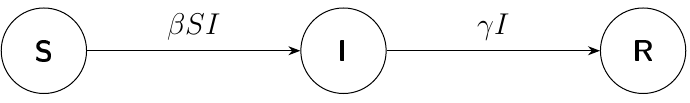
\includegraphics[width=0.7\textwidth]{Graphics/sir_graph.png}
    \caption{Grafo del modelo compartimental SIR.}
    \label{fig:grafo-sir}
\end{figure}

Es fundamental que la modelación de estos flujos preserve coherencia en la representación matemática: cada transferencia entre compartimentos debe estar reflejada 
simétricamente como salida en una ecuación y entrada en otra. Si un flujo aparece restando en una ecuación pero no sumando en otra, se estaría introduciendo una 
pérdida neta de cantidad sin justificación física o biológica, lo cual constituye un error en la formulación del modelo compartimental. Esta correspondencia entre el 
grafo y el sistema de ecuaciones asegura, por ejemplo, la conservación de la cantidad total cuando el sistema así lo requiere, y ofrece además una interpretación 
estructural clara del proceso dinámico.

Cabe mencionar que también pueden existir flujos externos que no provienen de otro compartimento, como nacimientos en una población o entradas de materia desde una 
fuente externa. En estos casos, el término correspondiente se incorpora directamente en la ecuación del nodo de destino, sin necesidad de que exista otro nodo de 
origen en el grafo.

Identificar la estructura del grafo compartimental es un paso fundamental en el proceso de modelado, ya que determina qué interacciones se consideran posibles dentro 
del sistema de EDOs compartimentales. Sin embargo, conocer dicha estructura no es suficiente. Las ecuaciones diferenciales asociadas incluyen parámetros que determinan 
la intensidad o velocidad de cada flujo, y estos parámetros, en general, no se conocen con antelación. Por ello, deben estimarse a partir de datos observados. Una de 
las técnicas para este propósito es el ajuste por mínimos cuadrados, que será presentado en la sección siguiente.

\section{Ajuste por Mínimos Cuadrados}
\label{sec:mincuad}

El método de mínimos cuadrados es una técnica matemática ampliamente utilizada para ajustar modelos a datos observados, cuyo objetivo es encontrar los 
parámetros de un modelo que mejor expliquen los datos disponibles. Este método consiste en minimizar la suma de los cuadrados de las diferencias entre 
los valores observados y los valores estimados por el modelo \cite{Stigler81}.

Dado un conjunto de \( m \) observaciones \(\{t_k, y_k\} \in \mathbb{R} \times \mathbb{R}^m\), una función modelo \( f(t, \mathbf{p}) \) dependiente de un vector de 
parámetros \( \mathbf{p} \in \mathbb{R}^k \), y una función de error definida por la diferencia entre el valor observado \( y_k \) y el valor predicho por el modelo 
\( f(t_k, \mathbf{p}) \), se define la función objetivo:

\[
SSR(\mathbf{p}) = \sum_{k=1}^{m} [y_k - f(t_k, \mathbf{p})]^2,
\]

donde \( SSR \) (por sus siglas en inglés, \textit{Sum of Squared Residuals}) representa la suma de los cuadrados de los residuos. El problema consiste en encontrar 
el vector de parámetros \( \mathbf{p}^* \) que minimiza esta suma, es decir:

\[
\mathbf{p}^* = \arg \min_{\mathbf{p}} SSR(\mathbf{p}).
\]

Este enfoque permite ajustar modelos paramétricos cuando se conoce la forma funcional general de la relación entre las variables. Al minimizar el error 
cuadrático medio, se obtiene una estimación de los parámetros que proporciona la mejor aproximación posible al conjunto de datos, bajo el supuesto de 
errores distribuidos normalmente.

En el contexto de este trabajo, el método de mínimos cuadrados se utilizará para estimar los valores de los parámetros presentes en las ecuaciones diferenciales 
de los sistemas compartimentales generados a partir de grafos. A partir de un conjunto de datos observados, se buscará minimizar la diferencia entre las 
soluciones del modelo y los datos, de modo que los parámetros ajustados representen de forma adecuada la dinámica observada.

En este caso, el modelo ya no está definido por una expresión explícita como \( f(t, \mathbf{p}) \), sino por un sistema de ecuaciones diferenciales cuya solución 
depende de los parámetros. Esto implica que, para cada evaluación del error en el proceso de optimización, es necesario resolver el sistema de EDOs asociado. 
Por tanto, la integración numérica se convierte en un componente central del procedimiento. A continuación se introduce los m\'etodos num\'ericos, que serán utilizados 
para calcular las soluciones aproximadas de estos sistemas diferenciales.

\section{M\'etodos Num\'ericos}
\label{sec:metodos-numericos}

Los sistemas de EDOs aparecen con frecuencia en la modelación de fenómenos dinámicos en diversas disciplinas científicas \cite{Boyce2012}. En la mayoría de los casos, 
estos sistemas no admiten soluciones analíticas, por lo que es necesario recurrir a métodos numéricos para obtener aproximaciones de su comportamiento a lo largo 
del tiempo \cite{Burden2011}.

Esta sección presenta dos enfoques clásicos de integración numérica que permiten resolver EDOs de forma eficiente y precisa, según las características del problema. 
En primer lugar, se introduce el método de Runge-Kutta \cite{Burden2011}, ampliamente utilizado por su simplicidad y buen desempeño en una amplia gama de aplicaciones. 
Posteriormente, se describen las Fórmulas de Diferenciación Inversa (BDF), que ofrecen una alternativa robusta para sistemas que presentan rigidez \cite{Hairer1996}. 
A continuación, se detalla el método de Runge-Kutta y sus principales propiedades.

\subsection{Runge-Kutta}

Los métodos de Runge-Kutta constituyen una familia de algoritmos numéricos diseñados para obtener soluciones aproximadas de ecuaciones diferenciales ordinarias. 
Estos métodos se basan en cálculos iterativos que permiten avanzar paso a paso en la solución del sistema. Dentro de esta familia, el método de Runge-Kutta de orden 
4 es ampliamente utilizado por su equilibrio entre precisión y eficiencia computacional \cite{Fehlberg70, DormandPrince80}.

El método Runge-Kutta con control del tamaño de paso se basa en la combinación de dos fórmulas de diferentes órdenes: una de cuarto y otra de quinto. Ambas se utilizan 
de forma simultánea en cada paso de integración. La estimación del error local de truncamiento se obtiene como la diferencia entre estas dos soluciones. Esta 
característica permite que el método implemente un mecanismo de control de paso adaptativo: si el error estimado supera una tolerancia establecida, el tamaño del paso 
se reduce; si el error es pequeño, el paso se incrementa. Este ajuste dinámico del paso hace que el método sea especialmente eficiente en regiones donde la solución 
varía lentamente, y preciso en zonas de alta variación \cite{HairerNorsettWanner93}.

Para una EDO de la forma:

\[
\frac{dy}{dt} = f(t, y), \quad y(t_0) = y_0,
\]

el método de Runge-Kutta de orden 4 clásico calcula una aproximación \( y_{n+1} \) mediante la siguiente fórmula:

\[
\begin{aligned}
k_1 &= f(t_n, y_n), \\
k_2 &= f\left(t_n + \frac{h}{2}, y_n + \frac{h}{2}k_1\right), \\
k_3 &= f\left(t_n + \frac{h}{2}, y_n + \frac{h}{2}k_2\right), \\
k_4 &= f(t_n + h, y_n + hk_3), \\
y_{n+1} &= y_n + \frac{h}{6}(k_1 + 2k_2 + 2k_3 + k_4),
\end{aligned}
\]

donde \( h \) es el tamaño del paso y los \( k_i \) son pendientes intermedias que evalúan la función \( f \) en distintos puntos del intervalo. Esta fórmula 
proporciona una estimación de cuarto orden, lo que significa que el error local de truncamiento es proporcional a \( h^5 \).

El método Runge-Kutta agrega una segunda estimación de quinto orden que permite estimar el error cometido en el paso. A partir de esa estimación, se decide si aceptar 
el paso, si el error es pequeño, o repetirlo con un valor de \( h \) reducido, si el error es grande. Esta propiedad lo hace particularmente útil cuando se trabaja 
con soluciones que tienen regiones con cambios rápidos y otras más suaves\cite{HairerNorsettWanner93}.

En este trabajo, el método Runge-Kutta se utilizará para resolver numéricamente los sistemas de ecuaciones diferenciales compartimentales generados a partir de grafos, 
especialmente en aquellos casos en los que el sistema no presenta rigidez y puede ser tratado eficientemente mediante un esquema explícito. Sin embargo, cuando los 
modelos compartimentales introducen escalas de tiempo muy distintas o propiedades que hacen al sistema rígido, será necesario recurrir a métodos más adecuados para 
tales situaciones. En la siguiente sección se presentarán las Fórmulas de Diferenciación Inversa, una alternativa robusta y estable para abordar este tipo 
de problemas.

\subsection{Fórmulas de Diferenciación Inversa}

Las Fórmulas de Diferenciación Inversa (\textit{Backward Differentiation Formulas}, BDF) son una familia de métodos implícitos multipaso para la integración numérica de 
EDOs, particularmente efectivos para resolver sistemas rígidos \cite{Gear71, HairerWanner96}. Una BDF de orden $s$ aproxima la 
derivada $y'(t_{n+1})$ utilizando los valores de la solución en $s+1$ puntos temporales anteriores y actuales: $t_{n+1}, t_n, \ldots, t_{n+1-s}$. La fórmula 
general es:
\[
\sum_{k=0}^{s} \alpha_k y_{n+1-k} = h \beta_0 f(t_{n+1}, y_{n+1}),
\]
donde $h$ es el tamaño del paso, y $\alpha_k, \beta_0$ son coeficientes que dependen del orden $s$. Al ser métodos implícitos (ya que $y_{n+1}$ aparece en ambos 
lados de la ecuación, a través de $f(t_{n+1}, y_{n+1})$), requieren resolver una ecuación en cada paso de tiempo, a menudo mediante métodos 
iterativos como Newton-Raphson\cite{BurdenFaires2011}.

La principal ventaja de los métodos BDF es su excelente estabilidad al resolver sistemas rígidos. Un sistema rígido es aquel que involucra escalas de tiempo muy 
diferentes, donde algunos componentes de la solución cambian muy rápidamente mientras otros lo hacen lentamente. En estos casos, los métodos explícitos como 
Runge-Kutta pueden requerir tamaños de paso extremadamente pequeños para evitar errores numéricos o inestabilidades. En cambio, los métodos BDF permiten utilizar 
pasos de integración mucho más grandes sin comprometer la precisión ni la estabilidad de la solución, lo que los convierte en una opción más eficiente para este 
tipo de problemas \cite{AscherPetzold98}.

Hasta este punto, se ha planteado el problema de estimar los parámetros de un modelo definido por un sistema de ecuaciones diferenciales, para lo cual es necesario 
resolver dichas ecuaciones en cada paso del proceso de ajuste. Esto justifica la introducción de los métodos de integración numérica, como Runge-Kutta y BDF, que 
permiten obtener soluciones aproximadas del sistema en función de los parámetros. Sin embargo, aún no se ha definido cómo construir el sistema dinámico en cuestión. 
Dado que la estructura del modelo compartimental no se conoce de antemano, es necesario generar distintas configuraciones posibles del sistema, lo cual equivale 
a explorar el espacio de grafos dirigidos que determinan qué compartimentos interactúan entre sí. Esta tarea, al implicar una búsqueda combinatoria compleja en el 
espacio de posibles grafos dirigidos, será abordada mediante el uso de algoritmos genéticos, que se introducen en la próxima sección como herramienta principal para 
la exploración estructural del sistema.

\section{Algoritmo Genético (AG)}
\label{sec:ag}

El Algoritmo Genético es una metaheurística de optimización y búsqueda inspirada en el proceso de selección natural y los principios de la genética biológica. 
Fue propuesto inicialmente por Holland \cite{Holland75} y posteriormente desarrollado y aplicado en una amplia variedad de contextos por diversos autores, 
entre ellos Goldberg \cite{Goldberg89}. Forma parte de la familia de los algoritmos evolutivos, los cuales han sido formalizados y sistematizados en obras como 
la de Eiben y Smith \cite{EibenSmith15}.

Los algoritmos genéticos se basan en la conservación y modificación de una población de soluciones candidatas, también llamadas individuos o cromosomas.

Cada individuo representa una posible solución al problema que se desea resolver, codificada en una estructura manipulable, como una cadena de bits, una lista de 
enteros, un grafo dirigido, entre otros. A cada solución se le asigna un valor de aptitud, conocido como \textit{fitness}, el cual cuantifica qué tan buena es con 
respecto a la función objetivo.

La población se modifica a lo largo de sucesivas generaciones mediante la aplicación iterada de operadores genéticos como la selección, el cruzamiento y la mutación. 
A través de estos mecanismos, se combinan y modifican estructuras existentes para explorar el espacio de búsqueda, con el objetivo de encontrar 
soluciones cada vez mejores.

En este trabajo, el algoritmo genético se utilizará para explorar el conjunto de posibles grafos dirigidos que definen modelos compartimentales. Cada individuo 
en la población representará un grafo, donde los nodos corresponden a compartimentos y los arcos representan flujos entre ellos. A partir de cada grafo, se construye 
un sistema de EDOs compartimentales que modela la dinámica del sistema. El desempeño de cada modelo se evalúa resolviendo este sistema y comparando la solución 
obtenida con los datos observados, mediante una función de aptitud. Esta función combina el error cuadrático medio entre las trayectorias simuladas y los datos 
originales, junto con penalizaciones por características estructurales no deseadas. Estas penalizaciones incluyen, por ejemplo, la no conservación de la población total 
y una complejidad excesiva del grafo, medida según la cantidad de aristas. Esta función compuesta permite favorecer modelos que no solo se ajusten bien a los datos, 
sino que también respeten principios estructurales deseables como simplicidad y coherencia dinámica.

En las siguientes secciones se describen con detalle los componentes fundamentales del algoritmo genético 
aplicado: los operadores de cruzamiento, mutación y selección, responsables de la evolución de la población de grafos a lo largo del proceso de optimización.

\subsection{Cruzamiento}

La función del operador de cruzamiento, también conocido como recombinación, es combinar la información de dos o más individuos seleccionados denominados padres, 
para generar nuevos individuos denominados hijos, que hereden características de ambos progenitores. Este proceso está inspirado en la reproducción sexual y tiene 
como objetivo explorar nuevas regiones del espacio de búsqueda, favoreciendo la diversidad genética dentro de la población \cite{Holland75}.

En contextos tradicionales donde los individuos se representan mediante vectores numéricos, existen operadores de cruzamiento bien conocidos como el 
cruzamiento aritmético o el \textit{Simulated Binary Crossover}, comúnmente utilizado en optimización continua \cite{DebAgrawal95}. Sin embargo, cuando los individuos 
representan estructuras más complejas como grafos dirigidos, es necesario adaptar el operador de cruzamiento a esta representación.

En este trabajo, cada individuo representa un grafo dirigido con una cantidad fija de nodos, correspondiente al número de variables observadas en los datos. El 
cruzamiento entre dos grafos consiste en generar un nuevo grafo que combine subestructuras de ambos padres. Existen diversas formas de implementar este operador 
sobre grafos; una de las más intuitivas es el cruzamiento por unión parcial, donde se toma un subconjunto de aristas del primer padre y otro subconjunto del segundo, 
y se combinan para formar un nuevo conjunto de aristas en el descendiente. 

La Figura~\ref{fig:cruzamiento-uparcial} muestra un ejemplo de cruzamiento por unión parcial.

\begin{figure}[htbp]
    \centering
    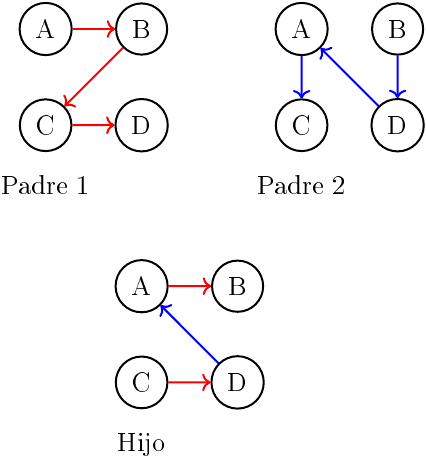
\includegraphics[width=0.35\textwidth]{Graphics/cruzamiento_pree_uparcial.png}
    \caption{Ejemplo de cruzamiento por unión parcial.}
    \label{fig:cruzamiento-uparcial}
\end{figure}

En el cruzamiento por intersección y expansión, se parte de las aristas comunes entre los dos padres y luego se añaden algunas aristas 
exclusivas de cada padre , seleccionadas aleatoriamente, manteniendo un equilibrio entre explotación y exploración. 

La Figura~\ref{fig:cruzamiento-intexp} muestra un ejemplo de cruzamiento por intersección y expansión.

\begin{figure}[htbp]
    \centering
    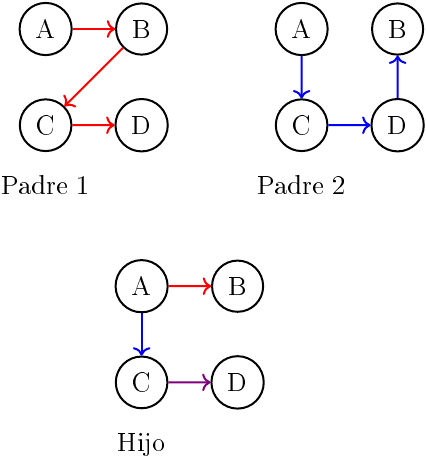
\includegraphics[width=0.35\textwidth]{Graphics/curzamiento_pree_intexp.png}
    \caption{Ejemplo de cruzamiento por intersección y expansión.}
    \label{fig:cruzamiento-intexp}
\end{figure}

La aplicación del cruzamiento en grafos permite generar nuevas topologías de modelos compartimentales, promoviendo la innovación estructural dentro del proceso 
evolutivo. Sin embargo, para evitar la convergencia prematura y fomentar la exploración del espacio de búsqueda, también es necesario introducir variaciones 
aleatorias en los hijos. Estas modificaciones puntuales se realizan a través del operador de mutación, el cual se describirá en la siguiente sección.


\subsection{Mutación}

El operador de mutación introduce variaciones aleatorias en los individuos de la población \cite{Goldberg89}. Su objetivo es mantener la diversidad dentro del 
algoritmo genético, evitando que la población converja prematuramente hacia soluciones subóptimas. A diferencia del cruzamiento, que combina información preexistente, 
la mutación genera nuevas características que no estaban presentes en los padres, permitiendo así una exploración más amplia del espacio de búsqueda.

En representaciones numéricas tradicionales, existen operadores como la mutación polinomial o la mutación gaussiana, que consisten en pequeñas perturbaciones sobre 
los valores de los genes \cite{DebBeyer01Final}. No obstante, cuando los individuos representan estructuras discretas como grafos, la mutación debe adaptarse a ese 
contexto.

La mutación aplicada a grafos consiste en modificar aleatoriamente su topología, afectando directamente los arcos que conectan los nodos. Algunas de las operaciones 
de mutación más comunes en este contexto incluyen:

\begin{itemize}
    \item \textbf{Adición de una arista:} se inserta un nuevo arco entre dos nodos que no estaban previamente conectados.
    \item \textbf{Eliminación de una arista:} se remueve un arco existente del grafo, simplificando su estructura.
    \item \textbf{Reversión de una arista:} se invierte la dirección de un arco existente, modificando el flujo entre compartimentos.
\end{itemize}

La Figura~\ref{fig:mutaciones-grafo-pree} muestra un ejemplo de cada una de las mutaciones mencionadas. 

\begin{figure}[htbp]
    \centering
    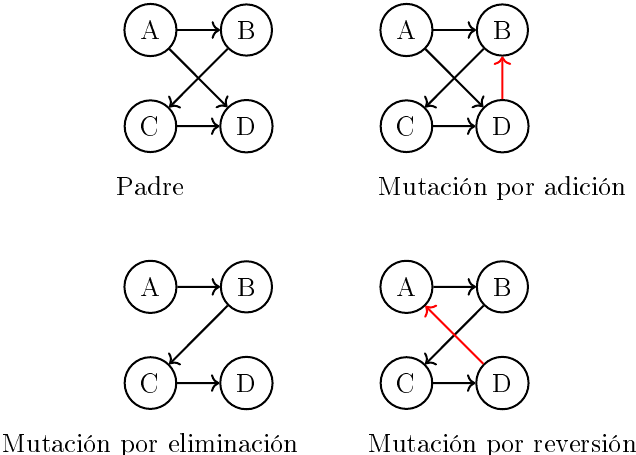
\includegraphics[width=0.5\textwidth]{Graphics/mutacion_pree.png}
    \caption{Ejemplo de mutaciones sobre grafo.}
    \label{fig:mutaciones-grafo-pree}
\end{figure}

Estas pequeñas modificaciones permiten que los hijos exploren regiones del espacio de grafos no alcanzables solo mediante cruzamiento, incrementando así la capacidad 
del algoritmo para descubrir modelos más adecuados. Las mutaciones se aplican típicamente con baja probabilidad, para evitar que la búsqueda se vuelva puramente 
aleatoria y pierda la dirección evolutiva basada en el desempeño.

Una vez generados y modificados los nuevos individuos, es necesario determinar cuáles serán preservados para la siguiente generación. Este proceso se lleva a cabo 
mediante el operador de selección, que se presentará en la próxima sección.


\subsection{Selección}

La selección es el proceso mediante el cual se eligen los individuos de la población actual que participarán en la generación de la siguiente. Este 
operador guía la presión evolutiva del algoritmo genético, favoreciendo la reproducción de aquellos individuos que presentan mayor desempeño según el \textit{fitness}. 
La probabilidad de ser seleccionado está relacionada directamente con la calidad de la solución, de modo que los modelos más prometedores tienen más oportunidades 
de transmitir sus estructuras a las generaciones futuras \cite{Goldberg89}.

Existen diversos métodos de selección, cada uno con características particulares. En la selección por ruleta, también llamada selección proporcional, 
la probabilidad de elegir un individuo es proporcional a su aptitud relativa dentro de la población. En la selección por torneo, se elige al azar un 
subconjunto pequeño de individuos y se selecciona el mejor entre ellos, un proceso que introduce competencia local. Finalmente, la selección por rango 
ordena a los individuos por aptitud y asigna probabilidades en función de su posición en el ranking, lo que suaviza las diferencias extremas y mantiene diversidad \cite{BlickleThiele96}.

Cuando los individuos representan grafos dirigidos, como en este trabajo, la función de aptitud depende no solo del ajuste del modelo a los datos 
medido mediante el error cuadrático medio, sino también de propiedades estructurales del grafo como su complejidad y la conservación de la población total. 
Por tanto, la selección favorece grafos que generan modelos compartimentales tanto precisos como coherentes desde el punto de vista dinámico y estructural.

Con el operador de selección se completa el ciclo evolutivo del algoritmo genético, permitiendo avanzar hacia generaciones sucesivas con individuos que combinan 
estructuras y comportamientos dinámicos. De esta manera, el algoritmo explora el espacio de modelos compartimentales.

Hasta aquí se han presentado los conceptos fundamentales necesarios para el desarrollo de esta tesis, incluyendo los sistemas de ecuaciones diferenciales, 
modelos compartimentales, métodos numéricos para su resolución, y el uso de algoritmos genéticos.

En el siguiente capítulo se describirá paso a paso cómo se construyen los sistemas de ecuaciones
diferenciales ordinarias compartimentales a partir de los grafos, y cómo se calcula el valor del \textit{fitness} que guía la evolución de las soluciones hacia modelos dinámicos.

\chapter{C\'alculo del \textit{Fitness}}\label{chapter:fitness}

En este capítulo se describe el procedimiento mediante el cual se evalúa la capacidad de un grafo dirigido para modelar un sistema compartimental que represente 
adecuadamente datos observacionales. Cada grafo candidato define de manera única un sistema de ecuaciones diferenciales ordinarias (EDOs), donde los nodos corresponden 
a compartimentos y las aristas representan interacciones entre ellos. A partir de la estructura del grafo y de las trayectorias temporales observadas, se construyen 
las ecuaciones dinámicas correspondientes, ajustando sus coeficientes mediante información extraída de los datos. Esta conversión permite evaluar computacionalmente 
qué tan bien el sistema de EDOs asociado al grafo logra reproducir la dinámica observada, a través de una función de \textit{fitness} que combina precisión en el 
ajuste, plausibilidad estructural y restricciones biológicas.

La sección~\ref{sec:exp_pol} introduce la generación inicial de ecuaciones polinomiales hasta segundo orden para cada compartimento, a partir de una biblioteca de términos 
construida de forma sistemática. En la sección~\ref{sec:term_sig} se detalla el procedimiento de selección de términos significativos, que consiste en ajustar los coeficientes 
por mínimos cuadrados, normalizar sus valores y filtrar aquellos de baja relevancia, manteniendo la coherencia estructural con el grafo. La sección~\ref{sec:cons_sis} 
explica cómo, a partir de los términos seleccionados y las conexiones topológicas del grafo, se construyen las ecuaciones diferenciales completas del sistema dinámico, 
y se describe cómo estas ecuaciones simbólicas se 
convierten en funciones numéricamente evaluables, permitiendo calcular trayectorias simuladas. Finalmente, en la sección~\ref{sec:punt_fit} se presenta la definición completa del 
\textit{fitness}, que incluye el cálculo del error cuadrático medio entre datos y simulaciones, junto con penalizaciones por comportamientos no deseados como 
poblaciones negativas, alta complejidad estructural o sobreconectividad del grafo.

A continuación, se describe el proceso de generación y filtrado de términos polinomiales que sirven como base para construir el sistema dinámico asociado a cada grafo.

\section{Expansión Polinómica del Modelo Dinámico}
\label{sec:exp_pol}

El cálculo del \textit{fitness} comienza con una matriz de datos temporales que describe la evolución de las poblaciones 
en cada compartimento a lo largo del tiempo y un grafo dirigido que representa las interacciones entre dichos compartimentos. 

Para cada compartimento, se generan ecuaciones que contienen todos los posibles términos  polinomiales hasta segundo orden. Esta construcción de una biblioteca de 
funciones candidatas a partir de la cual se seleccionará la estructura del modelo es una práctica establecida en la identificación de sistemas dinámicos no lineales 
\cite{ljung1999, Billings2013}. Los términos considerados son:

\begin{itemize}
    \item Términos lineales del tipo $X_i$, donde $X_i$ es la variable asociada al compartimento $i$.
    \item Términos cuadráticos del tipo $X_i X_j$ para todas las combinaciones posibles de compartimentos $i$ y $j$, incluyendo productos consigo mismos.
\end{itemize}

Por ejemplo, en un sistema con \(X_0, X_1, X_2\) donde cada uno de estos compartimentos representan un nodo del grafo, las ecuaciones asociadas a cada nodo serían:
\begin{align*}
    \frac{dX_0}{dt} &= a_{00} X_0 + a_{01} X_1 + a_{02} X_2 + a_{03} X_0^2 + a_{04} X_0 X_1 + a_{05} X_0 X_2 + a_{06} X_1^2 + a_{07} X_1 X_2 + a_{08} X_2^2, \\
    \frac{dX_1}{dt} &= a_{10} X_0 + a_{11} X_1 + a_{12} X_2 + a_{13} X_0^2 + a_{14} X_0 X_1 + a_{15} X_0 X_2 + a_{16} X_1^2 + a_{17} X_1 X_2 + a_{18} X_2^2, \\
    \frac{dX_2}{dt} &= a_{20} X_0 + a_{21} X_1 + a_{22} X_2 + a_{23} X_0^2 + a_{24} X_0 X_1 + a_{25} X_0 X_2 + a_{26} X_1^2 + a_{27} X_1 X_2 + a_{28} X_2^2.
\end{align*}

La inclusión sistemática de estos términos se inspira en técnicas clásicas de modelado de sistemas dinámicos, donde los términos lineales permiten representar 
efectos proporcionales como tasas constantes de crecimiento o pérdida \cite{strogatz2018nonlinear}, mientras que los términos cuadráticos capturan interacciones 
no lineales entre compartimentos, tales como competencia \cite{murray2002mathematical}, cooperación o transmisión \cite{anderson1992infectious}. 

Este conjunto base de funciones puede entenderse como una expansión polinómica de orden dos, similar a una serie de Taylor truncada \cite{ArfkenWeberHarris2012}, 
diseñada para capturar la dinámica local del sistema mediante combinaciones algebraicas con complejidad acotada. Al incluir desde el inicio todos los términos 
polinomiales de primer y segundo orden que puedan influir en la evolución del sistema, se evita descartar prematuramente posibles interacciones relevantes.

Este paso proporciona una base estructurada sobre la cual se realiza, en la próxima sección, la selección de los términos significativos que son aquellos que 
resultan relevantes para describir la dinámica observada.

\section{Selección de Términos Significativos}
\label{sec:term_sig}

Una vez generadas las ecuaciones expandidas para cada compartimento, el siguiente paso consiste en ajustar sus coeficientes y seleccionar los términos significativos. 
La relevancia de un término se determina en función de la magnitud y el signo de su coeficiente tras el ajuste, así como de su coherencia con la topología del grafo. 
Este proceso se desarrolla en tres etapas: ajuste de coeficientes, eliminación de términos no significativos, e identificación de términos compartidos entre 
compartimentos conectados.

Para cada ecuación, se estiman las derivadas numéricas de los datos originales utilizando diferencias finitas hacia adelante, lo que permite aproximar las 
tasas de cambio temporales. Por ejemplo, si se dispone de datos de población para el compartimento \(X_1\) 
en los tiempos \(t_0\) y \(t_1\), la derivada en \(t_0\) se puede calcular como:
\[
\dot{X}_1(t_0) \approx \frac{X_1(t_1) - X_1(t_0)}{\Delta t}.
\]
Para el último punto de la serie temporal, se utiliza una fórmula de diferencia finita hacia atrás:
\[
\dot{X}_1(t_{n-1}) \approx \frac{X_1(t_{n-1}) - X_1(t_{n-2})}{\Delta t}.
\]

A continuación, se construye una matriz que contiene la evaluación de cada término algebraico en cada instante de tiempo. Esta matriz permite reformular el 
problema como un sistema lineal, donde los coeficientes de la ecuación diferencial son las incógnitas, y la derivada numérica actúa como vector objetivo. 
Este enfoque es común en la identificación de sistemas dinámicos \cite{ljung1999, Billings2013}.

Por ejemplo, si una ecuación incluye los términos \(X_0\), \(X_1\) y \(X_0 X_1\), y se tienen observaciones en 4 puntos de tiempo, entonces la matriz de diseño 
tendrá 4 filas y 3 columnas, donde cada entrada corresponde al valor del término evaluado en ese instante. El sistema se resuelve mediante mínimos cuadrados para 
encontrar los coeficientes que minimizan la diferencia entre las derivadas observadas y las predichas.

Los coeficientes obtenidos se normalizan al intervalo \([0, 1]\), conservando el signo original. Esta normalización facilita la comparación entre términos 
y permite interpretar la magnitud relativa de cada interacción \cite{Bishop2006, Hastie2009}.  Preservar los signos es importante, ya que indica la dirección del 
flujo: coeficientes positivos representan aportes a un compartimento, mientras que valores negativos corresponden a salidas.

Tras el ajuste, se eliminan todos los términos cuyo coeficiente sea inferior a un umbral predefinido. Este umbral actúa como un hiperparámetro que regula el equilibrio 
entre la complejidad del modelo y su capacidad de ajuste. Por ejemplo, si el umbral es 0.1, el término $0.05 X_2^2$ sería eliminado por considerarse no significativo. 
Un umbral bajo puede conducir a modelos con demasiados términos irrelevantes y, por ende, propensos al sobreajuste \cite{Hastie2009}. Por el contrario, un umbral 
excesivamente alto podría descartar interacciones relevantes.  Esta técnica de eliminación de términos basada en la magnitud de sus coeficientes es una forma de 
selección de variables o reducción de la complejidad del modelo \cite{Billings2013, Hastie2009}.

La eliminación de t\'erminos no significativos responde al principio de parsimonia en modelado matemático \cite{Burnham2002, Box1976}, priorizando modelos más simples 
y comprensibles sin sacrificar precisión. El resultado es un conjunto reducido de términos con impacto significativo en la dinámica poblacional observada.

Después de eliminar los términos no relevantes, se comparan las ecuaciones de los nodos que están conectados entre sí en el grafo. Se identifican los términos que 
aparecen simultáneamente en ambas ecuaciones; por ejemplo, si los compartimentos \(X_1\) y \(X_2\) están conectados, sus ecuaciones diferenciales respectivas luego 
del ajuste y selección de términos significativos quedan como:
\begin{align*}
\frac{dX_1}{dt} &= 0.5 X_1 + 0.2 X_1 X_2 + 0.1 X_2^2, \\
\frac{dX_2}{dt} &= -0.4 X_2 + 0.3 X_1 X_2 + 0.2 X_1^2.
\end{align*}
El término \(X_1 X_2\) aparece en ambas ecuaciones, indicando una interacción directa entre los compartimentos. Por tanto, este término 
se conserva como representativo de la influencia mutua modelada por la arista entre \(X_1\) y \(X_2\).

En caso de que no existan términos comunes entre dos nodos conectados, se introduce al menos un término que combine sus variables, como \(X_i X_j\). Esto garantiza 
que toda conexión topológica en el grafo tenga una contraparte algebraica en el sistema de ecuaciones. Así se mantiene la coherencia entre la estructura del grafo y la 
formulación matemática del modelo. Esta adición no es arbitraria: el término \(X_i X_j\) tiene una interpretación natural como interacción entre las poblaciones de 
ambos compartimentos. Por ejemplo, \(X_0\) y \(X_3\) están conectados en el grafo, pero después del filtrado de términos significativos no comparten ningún término y 
sus respectivas ecuaciones quedan como las siguientes: 
\begin{align*}
\frac{dX_0}{dt} &= 0.6 X_0 - 0.2 X_1^2, \\
\frac{dX_3}{dt} &= -0.5 X_3 + 0.1 X_2 X_3.
\end{align*}
Entonces, para asegurar la representación dinámica de esa conexión, se incorpora el término \(X_0 X_3\) como representativo en ambas ecuaciones, que refleja la 
interacción entre \(X_0\) y \(X_3\), en concordancia con la arista existente entre ellos en el grafo. De esta manera, se evita que la estructura topológica pierda 
validez dinámica en el modelo.

Este mecanismo garantiza que las conexiones entre compartimentos deben estar respaldadas por interacciones en las ecuaciones que reflejen adecuadamente los posibles 
flujos o influencias entre ellos.

El siguiente paso consiste en construir formalmente el sistema dinámico completo. Esta reconstrucción se realiza a partir de los elementos obtenidos hasta ahora: 
los términos significativos entre las ecuaciones, las conexiones del grafo y los coeficientes ajustados. En la próxima sección se describe en detalle cómo se generan 
las ecuaciones diferenciales a partir de estos componentes.

\section{Construcción del Sistema Dinámico Basado en el Grafo}
\label{sec:cons_sis}

Despu\'es de seleccionados los términos significativos, se procede a construir el sistema dinámico definitivo, en el cual las ecuaciones de cada compartimento se ajustan 
según la estructura topológica del grafo propuesto. Este proceso consta de tres etapas: la reconstrucción estructurada de las ecuaciones y el reajuste de coeficientes 
en el nuevo modelo y la conversión del sistema en funciones computables que permitan calcular las derivadas en cada instante de tiempo como parte de una integración 
diferencial mediante métodos numéricos.

Para cada compartimento, se genera una ecuación que incluye únicamente aquellos términos derivados de interacciones con otros nodos a los que está conectado 
directamente mediante una arista. La dirección de la arista influye directamente en la construcción de las ecuaciones: si el flujo va desde otro nodo hacia el 
nodo actual, los términos asociados tienen coeficientes positivos, indicando una contribución entrante; en cambio, si la arista sale del nodo, los coeficientes 
correspondientes son negativos, reflejando una pérdida o salida desde ese compartimento. Si el nodo \(X_1\) está conectado con \(X_0\) y \(X_2\) a través de las 
aristas \(X_0 \rightarrow X_1\) y \(X_1 \rightarrow X_2\), entonces su ecuación podrá contener términos como \(+a X_0\), \(+b X_0 X_1\) y \(-c X_1\), \(-d X_1 X_2\). 
Así, la ecuación de \(X_1\) podría tomar la forma:
\[
\frac{dX_1}{dt} = a X_0 + b X_0 X_1 - c X_1 - d X_1 X_2,
\]
donde los coeficientes \(a\), \(b\), \(c\), y \(d\) son positivos, y el signo con el que aparecen en la ecuación refleja si la interacción representa una ganancia 
o una pérdida para el nodo \(X_1\).

El modelo resultante mantiene así la consistencia estructural del grafo, en el sentido de que ningún nodo es influido por otros si no existe una conexión directa, 
lo que proporciona interpretabilidad y transparencia a las interacciones modeladas.

Tras la reconstrucci\'on de las ecuaciones, se realiza un nuevo ajuste de coeficientes mediante m\'etodos de m\'inimos cuadrados. Esta regresi\'on se aplica solo 
sobre el subconjunto de t\'erminos seleccionados y permitidos por la topolog\'ia, a fin de refinar los par\'ametros y mejorar el ajuste a las derivadas observadas.
Por ejemplo, si la ecuaci\'on de $X_1$ se reduce a $\dot{X}_1 = aX_0 - bX_1X_2$, los valores de $a$ y $b$ se recalculan para minimizar la diferencia entre la 
derivada observada y la predicha. Este enfoque de selecci\'on seguida de reajuste se asemeja a t\'ecnicas como \textit{LASSO} \cite{Tibshirani1996} o regresi\'on 
\textit{stepwise} \cite{Efroymson1960}, pero adaptado al contexto estructural impuesto por el grafo. As\'i se equilibra la interpretabilidad del modelo con su capacidad 
predictiva.

Un ejemplo de un grafo con tres nodos \(X_0\), \(X_1\), y \(X_2\), conectados mediante las aristas \(X_0 \rightarrow X_1\), \(X_1 \rightarrow X_2\), y 
\(X_0 \rightarrow X_2\). Tras el proceso de selección, reconstrucción y reajuste de coeficientes descrito, las ecuaciones del sistema dinámico podrían 
tomar la siguiente forma:
\begin{align*}
\frac{dX_0}{dt} &= -0.2 X_0 - 0.1 X_0 X_1 - 0.4 X_2, \\
\frac{dX_1}{dt} &= 0.2 X_0 + 0.1 X_0 X_1 - 0.6 X_1 - 0.3 X_1 X_2, \\
\frac{dX_2}{dt} &= 0.4 X_2 + 0.6 X_1 + 0.3 X_1 X_2.
\end{align*}
En este ejemplo, los signos reflejan la dirección del flujo: \(X_0\) pierde población hacia \(X_1\) y \(X_2\), lo que se refleja en términos negativos en su 
ecuación. A su vez, \(X_1\) recibe flujo desde \(X_0\) y lo envía hacia \(X_2\), resultando en una combinación de términos positivos y negativos. Finalmente, 
\(X_2\) actúa como sumidero en este grafo, acumulando los flujos entrantes desde \(X_0\) y \(X_1\).

Una vez definidos los términos y reajustados sus coeficientes, las ecuaciones se convierten de su forma simbólica a funciones evaluables numéricamente. Esta conversión 
es necesaria porque permite calcular el valor de las derivadas en cada instante de tiempo, lo cual es fundamental para poder integrar el sistema de ecuaciones y 
comparar los resultados con los datos observados. Para la manipulación algebraica se utiliza la biblioteca \texttt{SymPy} \cite{SymPy2017}, y su función 
\texttt{lambdify} permite transformar las expresiones simbólicas en funciones eficientes que pueden ser evaluadas directamente por algoritmos numéricos.

El resultado es un sistema de ecuaciones diferenciales ordinarias que puede ser evaluado computacionalmente. Esta capacidad es clave para calcular el error cuadrático 
medio (\textit{mean squared error}, MSE), el cual compara las soluciones del sistema con los datos reales. Dicho error se usa para asignar un puntaje de \textit{fitness} 
al sistema de ecuaciones construido, cuantificando qué tan bien el modelo representado por el grafo de entrada logra reproducir la dinámica observada. A continuación, 
se describe detalladamente este proceso de puntaje del \textit{fitness}.

\section{Puntaje del \textit{Fitness}}
\label{sec:punt_fit}

Ya construidas las ecuaciones diferenciales para cada compartimento, se evalúa su capacidad para reproducir los datos observados. Este proceso se realiza mediante 
integración numérica del sistema y posterior comparación entre las trayectorias simuladas y los datos originales. El resultado se expresa en un puntaje de 
\textit{fitness} que guía el proceso evolutivo.

El sistema de ecuaciones diferenciales se resuelve numéricamente utilizando la función \texttt{solve\_ivp} de la biblioteca \texttt{SciPy} \cite{Virtanen2020SciPy}. El método inicial empleado es 
\texttt{RK45}.

Una vez obtenidas las trayectorias simuladas, se calcula el error cuadrático medio (MSE) entre estas trayectorias y los datos originales. El MSE es especialmente 
adecuado como métrica de comparación porque penaliza de manera más severa las grandes desviaciones, lo que lo convierte en una función objetivo sensible al ajuste
y es ampliamente utilizado en problemas de regresión y ajuste de modelos \cite{Hastie2009, Bishop2006}.

A este error base se le añaden penalizaciones que incorporan restricciones biológicas, estructurales y computacionales, con el fin de guiar el proceso hacia modelos 
más plausibles. Las penalizaciones son las siguientes:

\begin{itemize}
    \item \textbf{No conservación de la población total:} Se penalizan soluciones en las que la población total varía, solo en caso de que el par\'ametro de 
    esta penalizaci\'on sea activado, bajo la hipótesis de un sistema cerrado sin nacimientos ni migraciones. La penalización se calcula como la varianza de la 
    masa total normalizada por el valor inicial:
    \[
    \text{penalización}_\text{masa} = \frac{\operatorname{Var}\left( \sum_i X_i(t) \right)}{\sum_i X_i(0)} \cdot \lambda_{\text{masa}}, \quad \lambda_{\text{masa}} = 10.
    \]

    \item \textbf{Presencia de valores negativos:} Se penaliza la aparición de poblaciones negativas, las cuales carecen de sentido físico. La penalización corresponde a la suma de los cuadrados de los valores negativos:
    \[
    \text{penalización}_\text{negativos} = \sum_{i,t} \min\left(X_i(t), 0\right)^2 \cdot \lambda_{\text{negativos}}, \quad \lambda_{\text{negativos}} = 5.
    \]

    \item \textbf{Complejidad estructural:} Se penaliza el número de aristas del grafo para favorecer modelos más simples. La penalización depende de la proporción cuadrática de aristas respecto al máximo posible:
    \[
    \text{penalización}_\text{estructura} = \text{MSE} \cdot \left(1 + \alpha \left( \frac{n_\text{aristas}}{n(n-1)} \right)^2 \right), \quad \alpha = 0.5.
    \]

    \item \textbf{Conectividad total del grafo:} Si el grafo tiene el número máximo de aristas dirigidas posibles, se aplica una penalización multiplicativa:
    \[
    \text{penalización}_\text{total} = \text{MSE} \cdot \beta, \quad \text{si } n_\text{aristas} = n(n-1), \quad \beta = 1.5.
    \]
\end{itemize}

El puntaje de \textit{fitness} final se define como la suma del error cuadrático medio y las penalizaciones aplicadas. Este valor refleja cuán bien el modelo describe 
los datos, considerando tanto precisión como simplicidad estructural. Un menor puntaje indica mejor desempeño.

En este capítulo se presentó el procedimiento detallado para evaluar la calidad de un modelo compartimental representado por un grafo dirigido. Se describió cómo, a 
partir de datos, se construyen ecuaciones diferenciales asociadas a cada compartimento mediante una combinación sistemática de términos polinomiales, 
los cuales se filtran en función de su relevancia. Luego, se explicó cómo se reconstruyen las ecuaciones conforme a la topología del grafo y 
cómo se ajustan los coeficientes de forma coherente con las direcciones del flujo. Finalmente, se definió una función de \textit{fitness} que cuantifica el grado de 
ajuste del sistema dinámico a los datos observados, incorporando penalizaciones que reflejan restricciones estructurales, biológicas y computacionales. Esta función 
actúa como el mecanismo de evaluación central para comparar distintas configuraciones de modelos compartimentales.

Contando ya con un procedimiento que permite asignar un puntaje de \textit{fitness} a cualquier sistema de ecuaciones diferenciales generado a partir de un grafo 
compartimental, el siguiente desafío consiste en explorar de manera eficiente el espacio de todos los posibles grafos que podrían representar la dinámica subyacente. 
Este problema de búsqueda estructural es abordado en el próximo capítulo mediante un algoritmo genético, una técnica evolutiva inspirada en la selección natural. A 
través de operadores como mutación, cruzamiento y selección, el algoritmo permite generar, modificar y evaluar poblaciones de grafos candidatos. El objetivo es 
identificar automáticamente estructuras de modelos que modele los datos observados.
\usetikzlibrary{matrix}
\chapter{Algoritmo Gen\'etico}\label{chapter:ga}

En este capítulo se describe el procedimiento completo mediante el cual un algoritmo genético es utilizado para explorar estructuras posibles de modelos 
compartimentales, representadas como grafos dirigidos, que se ajusten a datos observados. El objetivo de esta búsqueda es identificar configuraciones 
estructurales que, al ser convertidas en sistemas de ecuaciones diferenciales ordinarias, permitan reproducir de manera precisa la dinámica observada en 
los datos experimentales. La naturaleza combinatoria del espacio de posibles grafos hace inviable una exploración exhaustiva, por lo que se recurre a estrategias 
evolutivas que permiten navegar dicho espacio de forma eficiente.

En la Sección~\ref{sec:init_gen} se introduce el proceso de inicialización, que establece las condiciones de partida para la ejecución del algoritmo y genera la 
población inicial de grafos candidatos. La Sección~\ref{sec:cross_gen} aborda las estrategias de recombinación empleadas para crear nuevas soluciones a partir de 
grafos existentes. En la Sección~\ref{sec:mut_gen} se explica cómo se introduce variación adicional mediante modificaciones puntuales en la estructura de los grafos. 
Finalmente, la Sección~\ref{sec:seleccion} presenta el criterio utilizado para decidir qué individuos permanecen en la población de una generación a otra y describe 
el funcionamiento general del ciclo evolutivo, que guía la búsqueda iterativa de soluciones cada vez más adecuadas.

A continuación, se describe el procedimiento de inicialización del algoritmo, donde se definen los parámetros de control y se genera la población inicial de grafos.

\section{Inicio del Algoritmo Genético}
\label{sec:init_gen}

El proceso comienza con la fase de inicialización, donde se definen los parámetros necesarios para ejecutar el algoritmo genético. Estos parámetros controlan 
el comportamiento general del algoritmo y su capacidad para explorar distintas soluciones \cite{Goldberg1989, Eiben2015}.

Primero, se establece el número de generaciones, que indica cuántos ciclos evolutivos se realizarán. Un ciclo evolutivo es el proceso completo en el que se 
generan nuevos individuos, se evalúan mediante la función \textit{fitness} y luego se seleccionan los mejores para formar la siguiente generación \cite{Goldberg1989}. 

Cada generación corresponde a una iteración del algoritmo, en la que se crean nuevos individuos, en este caso grafos, a partir de los existentes. También se define 
el tamaño de la población, que es la cantidad de grafos que existirán simultáneamente en cada generación.

Otros parámetros importantes son las tasas de cruzamiento y de mutación. La tasa de cruzamiento determina cuántos grafos nuevos se crearán combinando partes de 
grafos anteriores, mientras que la tasa de mutación establece cuántos grafos modifica aleatoriamente para introducir nuevas variantes \cite{Holland1992, Goldberg1989}. 
Estos dos mecanismos exploran el espacio de soluciones y evitar que el algoritmo se estanque en óptimos locales \cite{Holland1992, Goldberg1989}. 

Además, se inicializa una estructura que almacena todos los grafos ya evaluados. Esta estructura permite evitar la repetición de soluciones y para que el algoritmo no 
explore siempre las mismas regiones del espacio de búsqueda \cite{Eiben2015}.

Tras definir los parámetros iniciales, se genera la población inicial. Cada individuo de esta población es un grafo dirigido que representa una posible 
estructura de modelo compartimental. Estos grafos se generan aleatoriamente y se representan mediante una matriz de adyacencia, en la cual una entrada en la 
posición $(i, j)$ indica la existencia de una arista dirigida desde el nodo $i$ hacia el nodo $j$.

Sin embargo, no cualquier grafo es válido. Debe cumplir dos condiciones: no puede contener conexiones de un nodo consigo mismo y debe ser conexo cuando se interpreta 
como grafo no dirigido. Esto asegura que todos los compartimentos del modelo estén interrelacionados y que ninguna parte del sistema quede aislada. Solo los grafos 
que cumplen estas condiciones y no han sido generados previamente se incorporan a la población inicial como candidatos válidos para ser evaluados.

Después de generar la población inicial y asegurar que todos los grafos cumplan con las condiciones establecidas, el siguiente paso es aplicar los mecanismos de 
cruzamiento y mutación. Estas operaciones, que se abordarán en las siguientes secciones, permiten modificar y combinar grafos con el objetivo de explorar nuevas 
estructuras y mejorar la calidad de los modelos compartimentales generados.

\section{Proceso de Cruzamiento}
\label{sec:cross_gen}

En esta implementación, el cruzamiento se basa en la técnica clásica de un punto, ampliamente utilizada en algoritmos genéticos \cite{Goldberg1989, Eiben2015}. El 
proceso comienza con la selección aleatoria de un punto de cruce, que corresponde a una fila dentro de la matriz de adyacencia del grafo. A partir de este punto, 
se construye una nueva matriz que contiene las filas superiores de un padre y las inferiores del otro. En la Figura~\ref{fig:cruzamiento-filas} se muestra un ejemplo 
de cruzamiento por filas con punto de cruce.

\begin{figure}[htbp]
\centering

\begin{tikzpicture}
    % Padre A
\node at (1.75,0.5) {Padre A};
\matrix (A) [matrix of nodes, nodes in empty cells,
nodes={minimum size=1cm, text centered, draw},
column sep=0.1cm, row sep=0.1cm, anchor=north west,
draw=black] at (0,0)
{
    \textcolor{blue}{0} & \textcolor{blue}{1} & \textcolor{blue}{0} \\
    \textcolor{blue}{0} & \textcolor{blue}{0} & \textcolor{blue}{1} \\
    \textcolor{blue}{1} & \textcolor{blue}{0} & \textcolor{blue}{0} \\
};
    
% Padre B
\node at (7.75,0.5) {Padre B};
\matrix (B) [matrix of nodes, nodes in empty cells,
nodes={minimum size=1cm, text centered, draw},
column sep=0.1cm, row sep=0.1cm, anchor=north west,
draw=black] at (6,0)
{
    \textcolor{red}{1} & \textcolor{red}{0} & \textcolor{red}{1} \\
    \textcolor{red}{1} & \textcolor{red}{1} & \textcolor{red}{0} \\
    \textcolor{red}{0} & \textcolor{red}{1} & \textcolor{red}{1} \\
};
    
    % Hijo
\node at (4.75,-4.0) {Hijo};
\matrix (H) [matrix of nodes, nodes in empty cells,
nodes={minimum size=1cm, text centered, draw},
column sep=0.1cm, row sep=0.1cm, anchor=north west,
draw=black] at (3,-4.5)
{
    \textcolor{blue}{0} & \textcolor{blue}{1} & \textcolor{blue}{0} \\
    \textcolor{blue}{0} & \textcolor{blue}{0} & \textcolor{blue}{1} \\
    \textcolor{red}{0} & \textcolor{red}{1} & \textcolor{red}{1} \\
};

\end{tikzpicture}
\caption{Ejemplo de cruzamiento con punto de cruce en la fila 2.}
\label{fig:cruzamiento-filas}
\end{figure}

Si este hijo del cruzamiento de punto de cruce por filas cumple con los criterios de validez mencionados en secciones anteriores, se agrega como parte de la población. 
En caso contrario, se intenta un segundo tipo de cruzamiento: el cruzamiento por columnas.

En este método alternativo, se selecciona un punto de corte vertical. La parte izquierda de la matriz del hijo proviene de un padre, y la parte derecha del otro. Este 
procedimiento también requiere validación posterior. La Figura~\ref{fig:cruzamiento-columnas} ilustra este segundo tipo de cruzamiento. Si tampoco cumple las 
condiciones de validez, el intento de cruzamiento se descarta y no se añade ningún nuevo individuo a la población desde esa pareja de padres.

\begin{figure}[htbp]
\centering
    
\begin{tikzpicture}
        % Padre A
\node at (1.75,0.5) {Padre A};
\matrix (A) [matrix of nodes, nodes in empty cells,
nodes={minimum size=1cm, text centered, draw},
column sep=0.1cm, row sep=0.1cm, anchor=north west,
draw=black] at (0,0)
{
    \textcolor{blue}{0} & \textcolor{blue}{1} & \textcolor{blue}{0} \\
    \textcolor{blue}{0} & \textcolor{blue}{0} & \textcolor{blue}{1} \\
    \textcolor{blue}{1} & \textcolor{blue}{0} & \textcolor{blue}{0} \\
};
        
    % Padre B
\node at (7.75,0.5) {Padre B};
\matrix (B) [matrix of nodes, nodes in empty cells,
nodes={minimum size=1cm, text centered, draw},
column sep=0.1cm, row sep=0.1cm, anchor=north west,
draw=black] at (6,0)
{
    \textcolor{red}{1} & \textcolor{red}{0} & \textcolor{red}{1} \\
    \textcolor{red}{1} & \textcolor{red}{1} & \textcolor{red}{0} \\
    \textcolor{red}{0} & \textcolor{red}{1} & \textcolor{red}{1} \\
};
        
        % Hijo
\node at (4.75,-4.0) {Hijo};
\matrix (H) [matrix of nodes, nodes in empty cells,
nodes={minimum size=1cm, text centered, draw},
column sep=0.1cm, row sep=0.1cm, anchor=north west,
draw=black] at (3,-4.5)
{
    \textcolor{blue}{0} & \textcolor{blue}{1} & \textcolor{red}{1} \\
    \textcolor{blue}{0} & \textcolor{blue}{0} & \textcolor{red}{0} \\
    \textcolor{blue}{1} & \textcolor{blue}{0} & \textcolor{red}{1} \\
};
    
\end{tikzpicture}
\caption{Ejemplo de cruzamiento con punto de cruce en la columna 2.}
\label{fig:cruzamiento-columnas}
\end{figure}

Al aplicar distintos métodos de recombinación, el algoritmo aumenta sus posibilidades de generar soluciones viables que podrían no surgir con un único tipo de 
cruzamiento \cite{Eiben2015}.

Una vez generados nuevos grafos mediante cruzamiento, estos se evalúan en la función \textit{fitness} y se incorporan a la población como posibles soluciones 
para la siguiente generación, lo cual es un paso estándar en el ciclo de los algoritmos genéticos \cite{Eiben2015}. A continuación, se describe el proceso de 
mutación y su papel en la diversidad genética del algoritmo.

\section{Proceso de Mutación}
\label{sec:mut_gen}

En el caso de que los individuos sean grafos dirigidos, existen tres tipos principales de mutaciones que se pueden aplicar directamente sobre su matriz de adyacencia:

\begin{itemize}
    \item \textbf{Eliminación de una arista}: se selecciona aleatoriamente una posición $(i,j)$ de la matriz que contiene un 1 
    (indicando una arista de \(X_i \rightarrow X_j\)) y se cambia a 0. Esta operación solo se ejecuta si no rompe la conexidad del grafo cuando se interpreta como no 
    dirigido.
    
    \item \textbf{Adición de una arista}: se escoge aleatoriamente una celda $(i,j)$ de la matriz de adyacencia que contenga un 0 y se cambia a 1, creando una nueva 
    arista dirigida \(X_i \rightarrow X_j\), siempre que esta conexión no exista previamente.

    \item \textbf{Cambio de dirección de una arista}: se elige una arista existente $(i,j)$, se elimina (poniendo un 0 en esa posición) y se añade la arista inversa 
    $(j,i)$ (poniendo un 1), siempre que esta última no esté ya presente.
\end{itemize}

La Figura~\ref{fig:mutaciones-ejemplo} ilustra estos tres tipos de mutación mediante operaciones sobre matrices de adyacencia.


\begin{figure}[htbp]
\centering
\begin{tikzpicture}
    
    % Original
\node at (1.75,1.5) {Original};
\matrix (O) [matrix of nodes, nodes in empty cells,
nodes={minimum size=1cm, text centered, draw},
column sep=0.1cm, row sep=0.1cm, anchor=north west,
draw=black] at (0,1)
{
    \textcolor{black}{1} & \textcolor{black}{1} & \textcolor{black}{0} \\
    \textcolor{black}{0} & \textcolor{black}{0} & \textcolor{black}{1} \\
    \textcolor{black}{1} & \textcolor{black}{0} & \textcolor{black}{0} \\
};
    
    % Mutación 1 - Eliminar arista (0,1)
\node at (9,1.5) {Mutación 1: Eliminar (0,1)};
\matrix (M1) [matrix of nodes, nodes in empty cells,
nodes={minimum size=1cm, text centered, draw},
column sep=0.1cm, row sep=0.1cm, anchor=north west,
draw=black] at (7,1)
{
    \textcolor{black}{1} & \textcolor{red}{0} & \textcolor{black}{0} \\
    \textcolor{black}{0} & \textcolor{black}{0} & \textcolor{black}{1} \\
    \textcolor{black}{1} & \textcolor{black}{0} & \textcolor{black}{0} \\
};
    
    % Mutación 2 - Agregar arista (1,0)
\node at (1.75,-4.0) {Mutación 2: Agregar (1,0)};
\matrix (M2) [matrix of nodes, nodes in empty cells,
nodes={minimum size=1cm, text centered, draw},
column sep=0.1cm, row sep=0.1cm, anchor=north west,
draw=black] at (0,-4.5)
{
    \textcolor{black}{1} & \textcolor{black}{1} & \textcolor{black}{0} \\
    \textcolor{red}{1} & \textcolor{black}{0} & \textcolor{black}{1} \\
    \textcolor{black}{1} & \textcolor{black}{0} & \textcolor{black}{0} \\
};
    
% Mutación 3 - Invertir dirección (2,0) -> (0,2)
\node at (9,-4.0) {Mutación 3: Invertir (2,0) $\rightarrow$ (0,2)};
\matrix (M3) [matrix of nodes, nodes in empty cells,
nodes={minimum size=1cm, text centered, draw},
column sep=0.1cm, row sep=0.1cm, anchor=north west,
draw=black] at (7,-4.5)
{
    \textcolor{black}{1} & \textcolor{black}{1} & \textcolor{red}{1} \\
    \textcolor{black}{0} & \textcolor{black}{0} & \textcolor{black}{1} \\
    \textcolor{red}{0} & \textcolor{black}{0} & \textcolor{black}{0} \\
};
    
\end{tikzpicture}
\caption{Ejemplos de mutaciones: eliminación, adición e inversión de aristas.}
\label{fig:mutaciones-ejemplo}
\end{figure}


En todos los casos, el grafo resultante debe cumplir con las restricciones estructurales del problema: debe permanecer conexo cuando se considera no dirigido y no debe 
haberse evaluado anteriormente. Para verificar que los grafos no han sido procesados se realiza una consulta en una tabla hash que almacena representaciones canónicas 
de los grafos ya analizados, y para comprobar la conexidad del sistema compartimental dado que los grafos en este contexto son dirigidos, la verificación de su 
conectividad se realiza sobre una versión no dirigida. Para ello, se construye una matriz simétrica \(A^{\text{undir}}\) combinando la matriz de adyacencia original 
\(A\) con su transpuesta mediante \(A^{\text{undir}}_{ij} = A_{ij} \lor A_{ji}\). Esta matriz representa un grafo no dirigido en el que se considera que hay conexión 
entre dos nodos si existe una arista en al menos una dirección. Usando la biblioteca \texttt{networkx} \cite{Hagberg2008}, se crea el grafo correspondiente y se aplica el método 
\texttt{is\_connected()} para comprobar que todos los nodos pertenecen al mismo componente conexo.

Si una mutación genera una estructura inválida ,por ejemplo un grafo evaluado anteriormente, el algoritmo descarta ese hijo y no lo agrega
a la población.

Una vez que se han generado nuevos grafos mediante cruzamiento y mutación, es necesario evaluar su calidad y decidir cuáles de ellos pasarán a la siguiente generación. 
No todos los individuos producidos en una iteración deben conservarse, por lo que se aplica un proceso de selección que permite retener aquellos grafos que mejor se 
ajustan a los datos. Esta etapa es clave para garantizar que el algoritmo evolucione hacia soluciones o\'ptimas lo que se aborda en la siguiente sección.

\section{Selección y evolución del algoritmo}
\label{sec:seleccion}

Después de aplicar las operaciones de cruzamiento y mutación, los nuevos grafos generados deben ser evaluados para determinar su capacidad de ajustarse a los datos. 
Esta evaluación se realiza con la función \textit{fitness}.

Solo se analizan los grafos que aún no han sido evaluados previamente, evitando así repeticiones innecesarias que no aportarían nueva información.

Los grafos nuevos se a\~naden a los de la generación anterior para formar una población ampliada. Esta población ampliada representa el conjunto completo de 
candidatos disponibles para la selección en la siguiente etapa. A esta población ampliada se le aplica un proceso de ordenamiento según el valor de \textit{fitness}, 
seleccionando los mejores $N$ individuos, donde $N$ es el tamaño original de la población inicial, para conformar la nueva generación. Este enfoque, conocido como 
selección elitista, garantiza que las soluciones prometedoras se conserven, mientras se incorporan también estructuras nuevas que pueden mejorar los resultados 
\cite{Eiben2015, Goldberg1989}.

Al finalizar todas las generaciones, el algoritmo retorna un conjunto de grafos con los mejores desempeños según la métrica de \textit{fitness}. Cada grafo describe 
cómo se conectan e interactúan los distintos compartimentos del modelo, determinando qué flujos de información o cantidad existen entre ellos.

En este capítulo se presentó el funcionamiento completo del algoritmo genético diseñado para explorar el espacio de modelos compartimentales representados por grafos 
dirigidos. Se detallaron los mecanismos que guían la evolución de la población de soluciones, incluyendo la generación inicial de grafos válidos, las operaciones de 
cruzamiento y mutación para introducir variabilidad estructural, y el proceso de selección que preserva los candidatos más prometedores. A lo largo del ciclo evolutivo, 
el algoritmo garantiza la validez topológica de los grafos, evita la repetición de individuos previamente evaluados y se orienta hacia configuraciones que maximizan la 
función de \textit{fitness}. Este enfoque evolutivo permite una búsqueda eficiente y estructurada de modelos dinámicos, manteniendo un equilibrio entre 
exploración del espacio de soluciones y explotación de los mejores resultados encontrados.

En el siguiente capítulo se presentan los experimentos y resultados obtenidos al aplicar la implementación propuesta a diferentes modelos compartimentales.
\chapter{Experimentos y resultados}\label{chapter:Results}

En este capítulo se presentan los experimentos realizados para evaluar
el desempeño y los resultados del algoritmo gen\'etico propuesta en este
trabajo para hallar el sistema de ecuaciones diferenciales ordinarias compartimentales que mejor se ajusten a un conjunto de datos.

En la sección~\ref{sec:experimentation1} se describe el marco experimental. La secci\'on~\ref{sec:experimentation2} muestra como se generaron los datos utilizados en los distintos experimentos y cómo se modeló la presencia de ruido en las muestras. En la sección~\ref{sec:experimentation3} se describen los experimentos realizados y sus resultados, y la secci\'on~\ref{sec:experimentation4} se analizan. A continuación se describe el marco experimental.


\section{Consideraciones en la etapa de experimentaci\'on}
\label{sec:experimentation1}
La presente tesis aborda el problema de identificar la estructura de un sistema de ecuaciones diferenciales compartimentales, lineales con respecto a los parámetros, que mejor se ajuste a un conjunto de datos observados. El espacio de búsqueda de posibles modelos compartimentales es combinatoriamente extenso, ya que cada topología de interconexiones entre compartimentos define un sistema de ecuaciones único. Para navegar eficientemente este vasto espacio de soluciones, se propone una metodología basada en \textbf{algoritmos genéticos}, donde cada posible sistema compartimental es representado mediante una estructura de grafo. La naturaleza estocástica y la carga computacional de los algoritmos genéticos, sumada a la necesidad de evaluar múltiples modelos candidatos en cada generación, justifica el uso de la infraestructura de cómputo de alto rendimiento para la experimentación. Las características del equipo donde se llevaron a cabo los experimentos se detallan a continuación.

\begin{itemize}
    \item \textbf{Servidor:} Dell EMC PowerEdge R640
    \item \textbf{Procesador (CPU):} 96 núcleos de cómputo
    \item \textbf{Memoria RAM:} 512 GB
    \item \textbf{Arquitectura:} 64 bits
    \item \textbf{Sistema Operativo:} Ubuntu 24.04
    \item \textbf{Uso de GPU:} No
\end{itemize}

La implementación algorítmica se desarrolló enteramente en el lenguaje de programación \textbf{Python} (versión 3.12). Se utilizaron bibliotecas especializadas y de amplio uso en la comunidad científica. Entre ellas destacan \textbf{NumPy} \cite{2020NumPy-Array} para operaciones matriciales de alto rendimiento; \textbf{SymPy} \cite{Meurer_SymPy_symbolic_computing_2017} para la construcción y manipulación simbólica de las ecuaciones diferenciales; y \textbf{SciPy} \cite{2020SciPy-NMeth} para la integración numérica de dichas ecuaciones para cada modelo candidato. De manera fundamental, se empleó la biblioteca \textbf{NetworkX} \cite{networkx} para modelar, construir y manipular las topologías de grafos que representan las interconexiones de los sistemas compartimentales. El núcleo de la solución, el \textbf{algoritmo genético} diseñado para evolucionar y encontrar la estructura del grafo óptima, fue una implementación propia desarrollada en el marco de esta investigación, y su código fuente se encuentra disponible en GitHub \cite{comparmentalodesystem2025}.

En la siguiente sección se detalla el procedimiento utilizado para la generación de los datos sintéticos que sirven como base para los experimentos.

\section{Descripci\'on del marco experimental}
\label{sec:experimentation2}

El proceso experimental comienza con la selección de un conjunto de modelos compartimentales conocidos, los cuales son utilizados como base para generar datos sintéticos que emulen escenarios observacionales realistas. Estos modelos representan diferentes estructuras epidemiológicas y varían tanto en complejidad como en número de compartimentos. En total, se consideraron cuatro modelos ampliamente utilizados en la literatura científica: \textbf{SIR}, \textbf{SEIR}, \textbf{SIRD} y \textbf{SEIRV}. Cada uno de ellos modela la evolución de una epidemia bajo distintos supuestos, incluyendo la exposición previa, la vacunación o la presencia de cuarentena y mortalidad.

Para cada modelo se establecieron condiciones iniciales y valores específicos para los parámetros, tomados de ejemplos clásicos o calibrados dentro de rangos razonables. Por ejemplo, para el modelo SIR se utilizó una población inicial distribuida como \( S_0 = 0.99 \), \( I_0 = 0.01 \) y \( R_0 = 0 \), con parámetros de transmisión \( \beta = 0.4 \) y recuperación \( \gamma = 0.1 \). El sistema de ecuaciones diferenciales correspondiente está dado por:

\[
\begin{aligned}
\frac{dS}{dt} &= -\beta SI, \\
\frac{dI}{dt} &= \beta SI - \gamma I, \\
\frac{dR}{dt} &= \gamma I.
\end{aligned}
\]

La integración de estos sistemas se realizó mediante el método \texttt{solve\_ivp} de la biblioteca \texttt{scipy.integrate}, evaluando las soluciones en 150 puntos equiespaciados dentro del intervalo temporal \( t \in [0, 150] \). Este enfoque proporciona una discretización suficiente para capturar la dinámica de los compartimentos sin generar una sobrecarga computacional innecesaria.

La Figura~\ref{fig:sir_sin_ruido} muestra la evolución simulada de los compartimentos del modelo SIR sin presencia de ruido, donde se observa claramente la transición típica entre susceptibles, infectados y recuperados.

\begin{figure}[htbp]
    \centering
    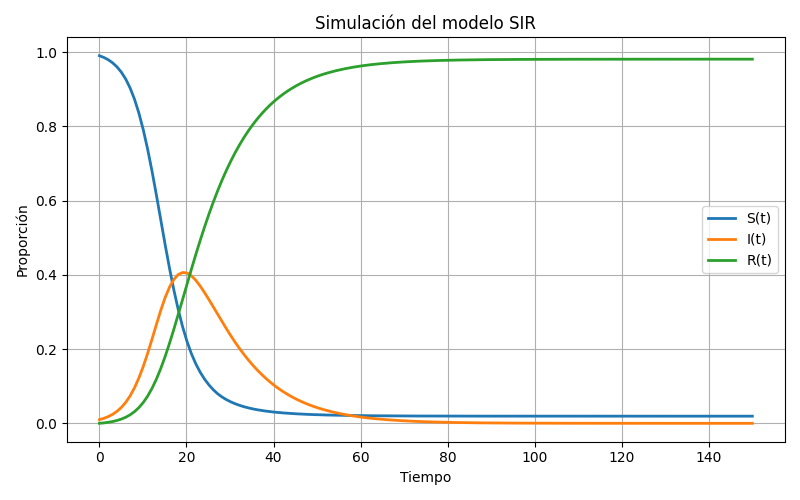
\includegraphics[width=0.7\textwidth]{Graphics/SIR_points.png}
    \caption{Simulación del modelo SIR sin ruido.}
    \label{fig:sir_sin_ruido}
\end{figure}

Una vez obtenidas las trayectorias libres de ruido para cada compartimento, se procedió a simular un entorno más cercano a situaciones reales introduciendo ruido aleatorio. Específicamente, se añadió ruido aditivo con distribución normal a cada punto de los datos. El nivel de ruido se controló mediante un parámetro denominado \texttt{max\_noise}, que representa la desviación estándar del ruido aplicado. Se consideraron tres niveles: 5\%, 15\,\% y 30\,\%, lo cual permite evaluar la robustez de los métodos posteriores frente a diferentes grados de perturbación. La expresión utilizada para generar los datos ruidosos fue:

\[
y_i^{\text{noise}} = y_i + \varepsilon, \quad \varepsilon \sim \mathcal{N}(0, \sigma),
\]

donde \( \sigma = \texttt{max\_noise} \). Cabe señalar que este tipo de ruido es aditivo y no proporcional al valor del compartimento, lo cual evita que variables pequeñas sean afectadas de manera desproporcionada.

La Figura~\ref{fig:sir_con_ruido} presenta una visualización de los datos del modelo SIR con un nivel de ruido del 30\,\%, donde se puede observar la dispersión introducida sobre los puntos originales, simulando así condiciones más próximas a mediciones empíricas.

\begin{figure}[htbp]
    \centering
    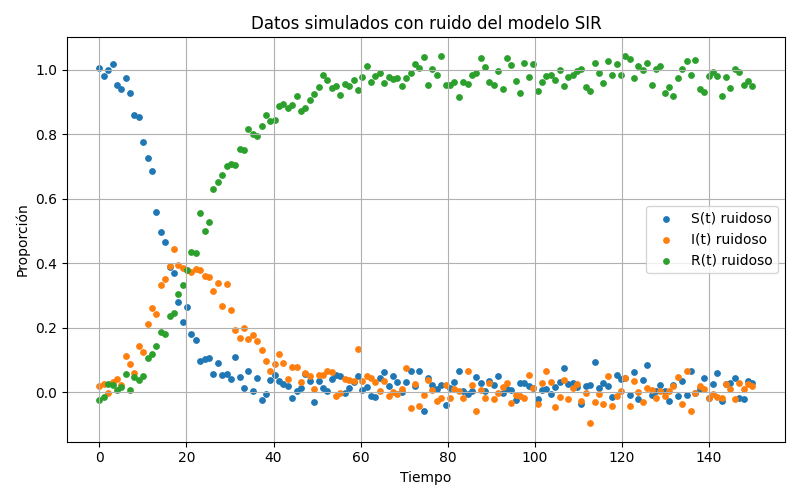
\includegraphics[width=0.7\textwidth]{Graphics/SIR_point_noise.png}
    \caption{Datos simulados del modelo SIR con ruido aditivo de nivel 3\,\%.}
    \label{fig:sir_con_ruido}
\end{figure}

Los conjuntos de datos generados se almacenaron como archivos \texttt{.csv}, con columnas correspondientes al tiempo y a cada compartimento del modelo. La nomenclatura de los archivos incluye el nombre del modelo y el nivel de ruido aplicado, facilitando su posterior identificación y análisis. En total, se produjeron 18 archivos (6 modelos combinados con 3 niveles de ruido), los cuales se emplean como entrada para las siguientes etapas del proceso, incluyendo ajuste de modelos, regresión simbólica y evaluación mediante algoritmos evolutivos.

Esta metodología de generación de datos proporciona un entorno controlado y reproducible para realizar pruebas experimentales, permitiendo estudiar de manera sistemática el desempeño de diferentes estrategias de modelado bajo condiciones con y sin ruido.

En la siguiente sección se presentan los resultados obtenidos en los experimentos realizados para los modelos \textbf{SIR}, \textbf{SEIR}, \textbf{SIRD}, \textbf{SEIRV} y \textbf{SIQRD}, con diferentes valores de ruido en los datos.

\section{Experimentos realizados}
\label{sec:experimentation3}

El experimento tiene como objetivo evaluar la capacidad de un algoritmo genético para inferir estructuras compartimentales, modeladas como sistemas de ecuaciones diferenciales ordinarias (EDOs), a partir de series temporales generadas por modelos epidémicos. Para ello, se desarrolló un marco computacional que transforma automáticamente grafos dirigidos en sistemas compartimentales, ajusta los coeficientes mediante mínimos cuadrados, y evalúa su capacidad predictiva sobre los datos originales.

Cada experimento parte de datos sintéticos generados por un modelo, a los cuales se les añade ruido aleatorio. Este ruido se introduce con diferentes distribuciones y niveles de intensidad, con el objetivo de analizar la robustez del algoritmo ante incertidumbre. Por cada combinación de configuración experimental se ejecutan 30 repeticiones independientes con semillas aleatorias distintas para garantizar diversidad estadística en los resultados.

El proceso de inferencia se realiza mediante un algoritmo genético que evoluciona grafos dirigidos válidos , cada uno representando una posible estructura compartimental. Los parámetros usados incluyen el tamaño de la población, la cantidad de generaciones, y las tasas de mutación y cruzamiento. A lo largo de la evolución, los individuos son evaluados mediante una función de \textit{fitness} basada en el error cuadrático medio (MSE) entre la simulación del modelo inferido y los datos observados. La función incluye penalizaciones adicionales por complejidad estructural, violación de la conservación poblacional, en caso de que se indique, y valores negativos en las simulaciones.

Se evaluaron también diferentes \textit{thresholds} que es el umbral que se define en el Cap\'itulo~\ref{chapter:fitness} en la Secci\'on~\ref{sec:term_sig} para seleccionar los t\'erminos relevantes en las ecuaciones, en este caso se usaron valores de 0.8 y 1.0, para controlar la significancia de los términos en las ecuaciones diferenciales, afectando así la complejidad de los modelos generados.

Por cada ejecución, se registran los siguientes elementos:
\begin{itemize}
    \item El mejor grafo descubierto y sus aristas.
    \item Las ecuaciones diferenciales finales generadas.
    \item El valor de fitness (MSE).
    \item El tiempo total de ejecución.
\end{itemize}

Los resultados obtenidos se presentan en una tabla resumen, donde se comparan las distintas configuraciones experimentales:

\begin{table}[H]
\centering
\caption{Resumen de resultados por configuración experimental}
\begin{tabular}{|c|c|c|c|c|}
\hline
\textbf{Ruido} & \textbf{\textit{Threshold}} & \textbf{Fitness Mín.} & \textbf{MSE} & \textbf{Aristas del grafo} \\
\hline
 &  &  &  &  \\
\hline
\end{tabular}
\label{tab:resultados-experimentales}
\end{table}

\noindent

Los valores de fitness representan el MSE entre la simulación del modelo inferido y los datos originales. Las métricas están promediadas sobre 30 ejecuciones independientes por configuración.

A continuación se presentan los resultados obtenidos para el modelo SIR.

\subsection{Modelo SIR}

El modelo SIR es un marco matemático fundamental que se utiliza para analizar cómo se propaga una enfermedad infecciosa a través de una población \cite{Kermack1927}. El sistema se define como:
\[
\begin{aligned}
\frac{dS}{dt} &= -\beta SI, \\
\frac{dI}{dt} &= \beta SI - \gamma I, \\
\frac{dR}{dt} &= \gamma I.
\end{aligned}
\]
donde S indica la cantidad de personas susceptibles, I la cantidad de personas infectadas y R la cantidad de personas recuperadas. Se utiliza el parámetro $\beta$ para indicar el índice de transmisión y $\gamma$ el índice de recuperación de la enfermedad.

El grafo que representar\'ia este sistema ser\'ia el compuesto por estas aristas: $S \rightarrow I$, $I \rightarrow R$.

Se utilizaron como valores de los parámetros $\beta = 0.4$ y $\gamma = 0.1$ con punto inicial (0.7, 0.3, 0) y se integró en el intervalo $0 \leq t \leq 150$ para obtener los datos que aparecen en la imagen~\ref{fig:sir_sin_ruido}. Del conjunto de puntos se seleccionaron 150 muestras como datos para el algoritmo gen\'etico. 

El algoritmo se ejecuto con los par\'ametros de 30 para la poblaci\'on inicial y 20 el n\'umero de geneaciones.

Los resultados obtenidos durante las 30 ejecuciones del algoritmo genético sobre los datos generados por el modelo SIR se resumen en la Tabla~\ref{tab:resumen-sir}. En ella se muestran las configuraciones correspondientes a diferentes niveles de ruido y valores de \textit{threshold} (0.8 y 1.0) utilizados para filtrar los términos significativos en las ecuaciones diferenciales. Para cada combinación se reporta el mejor valor de \textit{fitness}, el error cuadrático medio (MSE) en validación y la estructura del grafo inferido.

\begin{table}[H]
\centering
\caption{Resumen de las mejores soluciones para el modelo SIR bajo distintas configuraciones}
\label{tab:resumen-sir}
\begin{tabular}{|c|c|c|c|c|}
\hline
\textbf{Ruido} & \textbf{\textit{Threshold}} & \textbf{Fitness} & \textbf{MSE Validación} & \textbf{Aristas del Grafo} \\
\hline
5\% & 0.8 & 0.00008170 & 0.00007718 & 0 $\rightarrow$ 1, 1 $\rightarrow$ 2 \\
5\% & 1.0 & 0.00141273 & 0.00133686 & 0 $\rightarrow$ 1, 1 $\rightarrow$ 2 \\
15\% & 0.8 & 0.12484250 & 0.10983983 & 0 $\rightarrow$ 2, 1 $\rightarrow$ 2, 2 $\rightarrow$ 1 \\
15\% & 1.0 & 0.00266643 & 0.00076029 & 0 $\rightarrow$ 1, 1 $\rightarrow$ 2 \\
30\% & 0.8 & 0.01876324 & 0.01529640 & 0 $\rightarrow$ 2, 1 $\rightarrow$ 2 \\
30\% & 1.0 & 0.01876324 & 0.01529640 & 0 $\rightarrow$ 2, 1 $\rightarrow$ 2 \\
\hline
\end{tabular}
\end{table}

Las ecuaciones diferenciales asociadas a las mejores soluciones por configuración es la siguiente:
\[
\begin{aligned}
\frac{dS}{dt} &= -0.40199\,S I, \\
\frac{dI}{dt} &= 0.29265\,S I - 0.10328\,I^2 - 0.09670\,I R, \\
\frac{dR}{dt} &= 0.10934\,S I + 0.10328\,I^2 + 0.09670\,I R.
\end{aligned}
\]
En las Figuras~\ref{fig:sir_5p_th08}, \ref{fig:sir_15p_th10} y \ref{fig:sir_30p_th10} se pueden observar las comparaciones entre los datos originales y las simulaciones generadas por los modelos inferidos. Otro sistema de ecuaciones que alcanz\'o buenos resultados en las aproximaci\'on de los datos fue:
\[
\begin{aligned}
\frac{dS}{dt} &= -0.39851\,S I, \\
\frac{dI}{dt} &= 0.23646\,S I - 0.146624\,I R, \\
\frac{dR}{dt} &= 0.16205\,S I + 0.14662\,I R,
\end{aligned}
\]
que representa el conjunto de puntos representados en la Figura~\ref{fig:sir_15p_th10}.

\begin{figure}[H]
\centering
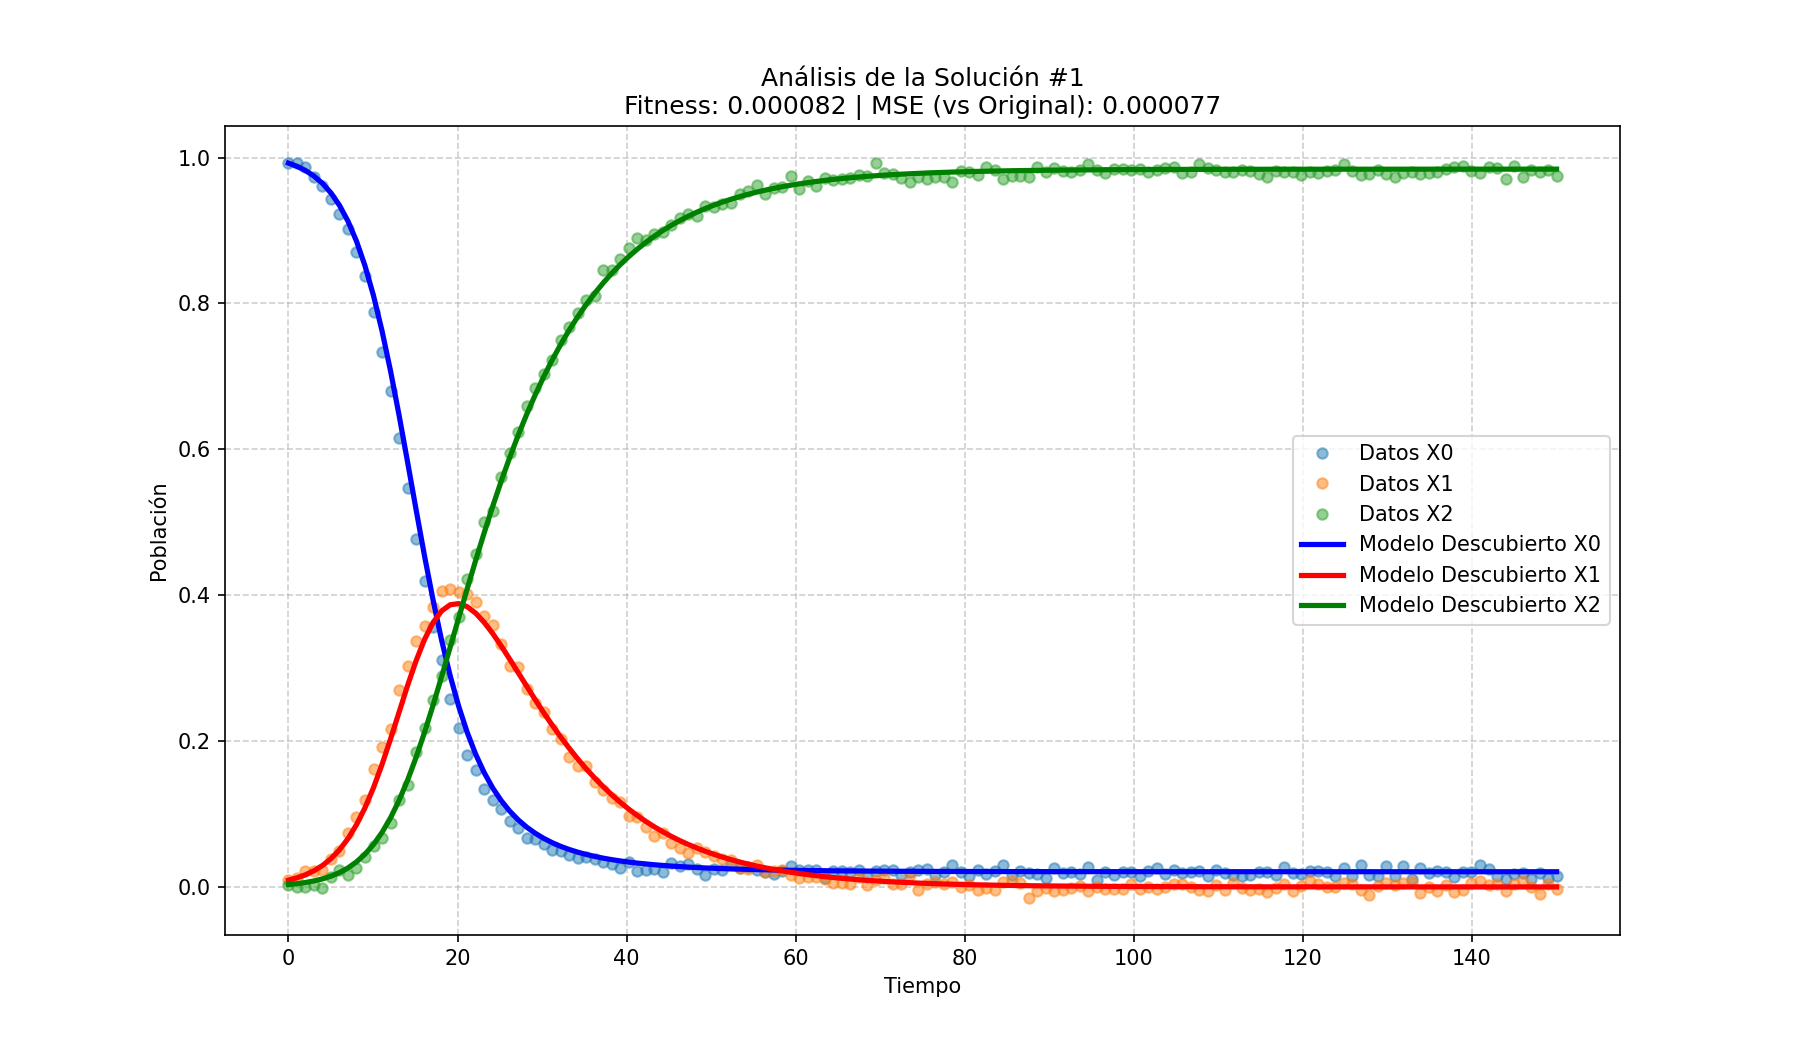
\includegraphics[width=0.7\textwidth]{Graphics/SIR_noise_0p005_0.8_exp10__solution_1.png}
\caption{Simulación del modelo vs datos reales para 5\% de ruido, \textit{threshold} 0.8. $X_0=S , X_1=I, X_2=R$}
\label{fig:sir_5p_th08}
\end{figure}

A pesar del ruido introducido en los datos, los resultados muestran que el sistema inferido logra aproximar adecuadamente el comportamiento dinámico original. En particular, con ruido del 5\,\% y un \textit{threshold} de 0.8, se obtuvo un modelo con error MSE de validación de apenas 7.7e-05 (Figura~\ref{fig:sir_5p_th08}), muy cercano a los datos originales. En contraste, para niveles de ruido más altos como el 30\,\%, aunque las ecuaciones inferidas presentan más términos ajenos al modelo SIR original, los valores de MSE siguen siendo razonables, como se aprecia en la Figura~\ref{fig:sir_30p_th10}.

\begin{figure}[H]
\centering
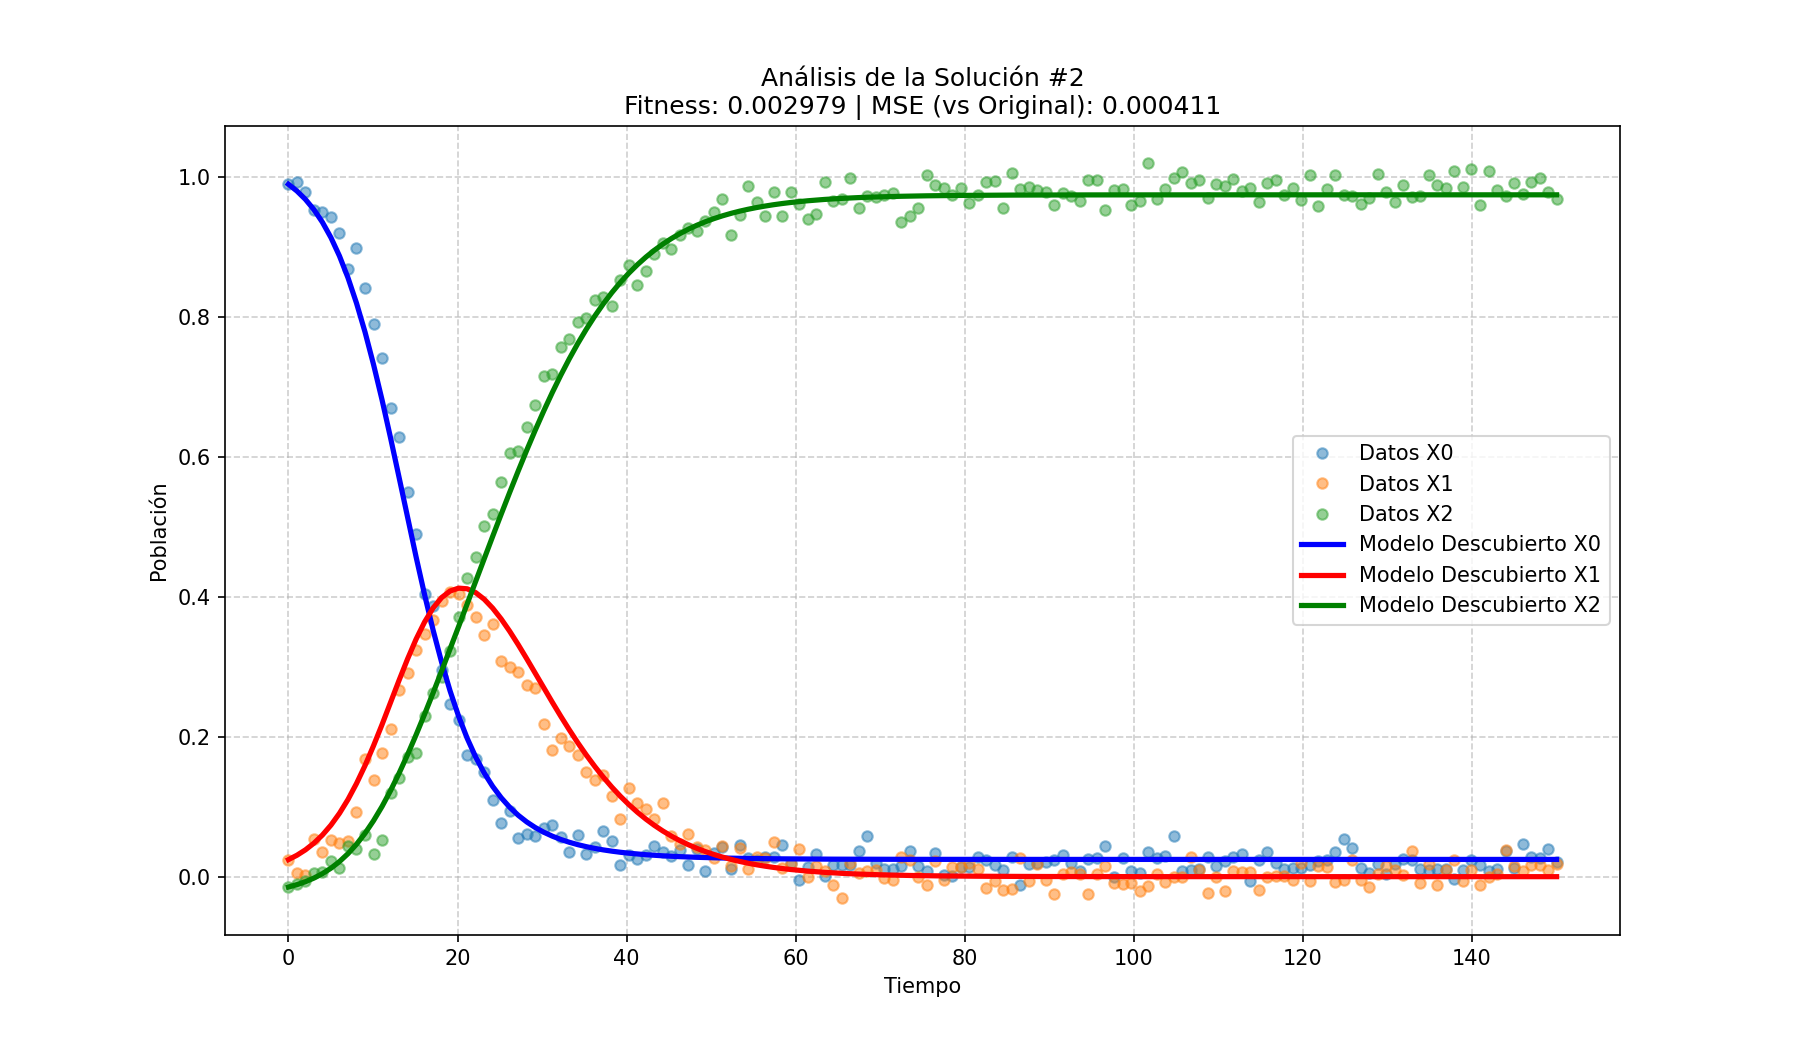
\includegraphics[width=0.7\textwidth]{Graphics/SIR_noise_0p015_1.0_exp10__solution_2.png}
\caption{Simulación del modelo vs datos reales para 15\% de ruido, \textit{threshold} 1.0. $X_0=S , X_1=I, X_2=R$}
\label{fig:sir_15p_th10}
\end{figure}

Es importante destacar que nunca se recuperó exactamente el sistema original que generó los datos. Sin embargo, los modelos inferidos son estructural y dinámicamente consistentes, respetando las restricciones del problema y capturando las tendencias generales del sistema. Esto se refleja en la cercanía entre las trayectorias simuladas y los datos reales en todos los escenarios evaluados. Adem\'as se devuelve correctamente el grafo que representa el modelo SIR.

\begin{figure}[H]
\centering
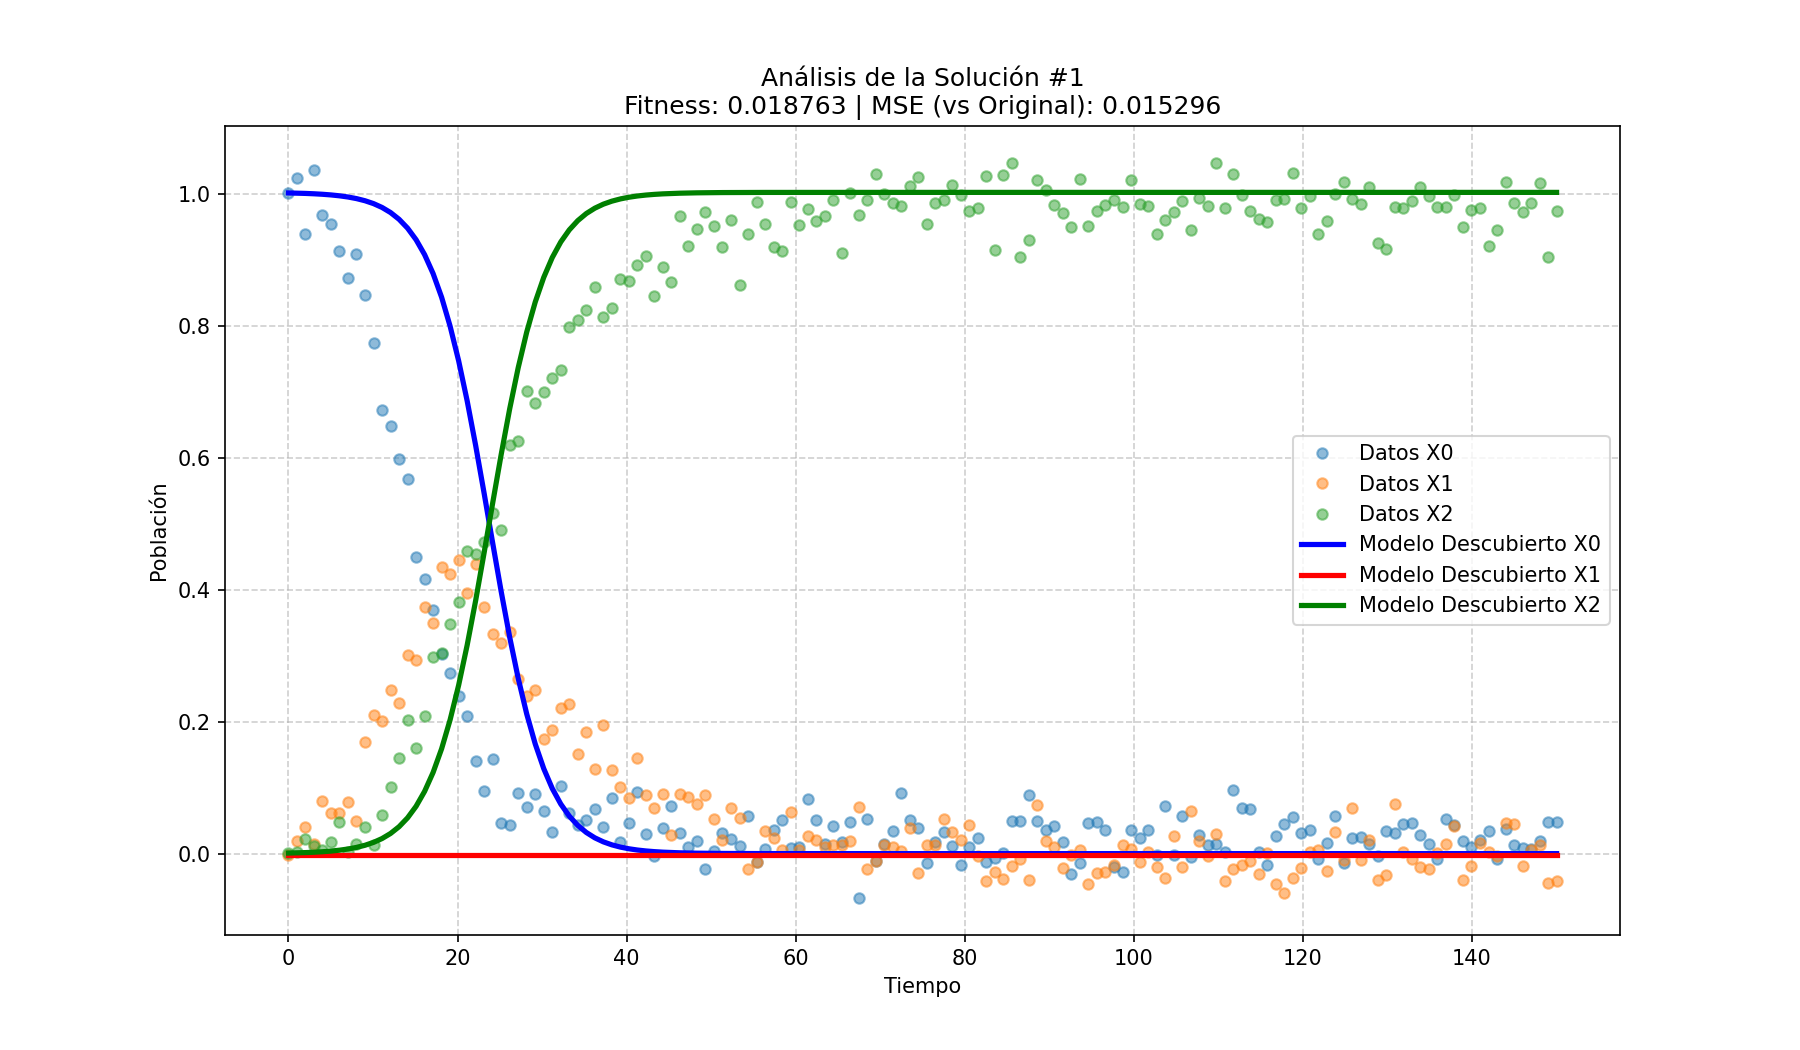
\includegraphics[width=0.7\textwidth]{Graphics/SIR_noise_0p03_1.0_exp18__solution_1.png}
\caption{Simulación del modelo vs datos reales para 30\% de ruido, \textit{threshold} 1.0. $X_0=S , X_1=I, X_2=R$}
\label{fig:sir_30p_th10}
\end{figure}

En condiciones ideales sin ruido y utilizando el sistema original como aproximador de derivadas, se logra una aproximación casi exacta, con valores promedio de fitness del orden de 1e-07.

Resaltar que los tiempos de ejecuci\'on durante cada ejecuci\'on del algoritmo gen\'etico van desde 40 segundos hasta 1 minuto. Estos tiempos son razonables teniendo en cuenta el espacio de b\'usqueda de todos los grafos v\'alidos.

A continuación se presentan los resultados en los experimentos del modelo SEIR.

\subsection{Modelo SEIR}

El modelo SEIR refina al clásico modelo SIR al incorporar un período de latencia de la enfermedad, proporcionando un marco matemático más realista para infecciones donde los individuos no se vuelven infecciosos inmediatamente después del contagio \cite{Hethcote2000}. El sistema se define mediante el siguiente conjunto de ecuaciones diferenciales:
%
\[
\begin{aligned}
    \frac{dS}{dt} &= -\beta SI, \\
    \frac{dE}{dt} &= \beta SI - \alpha E, \\
    \frac{dI}{dt} &= \alpha E - \gamma I, \\
    \frac{dR}{dt} &= \gamma I.
\end{aligned}
\]
%
Donde S representa la proporción de individuos susceptibles, E los expuestos (en período de incubación y no infecciosos), I los infecciosos y R los recuperados. El parámetro $\beta$ controla la tasa de transmisión, $\alpha$ es la tasa a la que los individuos expuestos se vuelven infecciosos, y $\gamma$ es la tasa de recuperación.

El grafo que representa este sistema está compuesto por las siguientes aristas, que ilustran las transiciones posibles entre los compartimentos: $S \rightarrow E \rightarrow I \rightarrow R$.

Se utilizaron como valores de los parámetros $\beta = 0.4$, $\alpha = 0.2$ y $\gamma = 0.1$ con punto inicial (0.9, 0.1, 0, 0) y se integró en el intervalo $0 \leq t \leq 150$ para obtener los datos que aparecen en la imagen~\ref{fig:seir_sin_ruido}. Del conjunto de puntos se seleccionaron 150 muestras como datos para el algoritmo genético.

\begin{figure}[H]
    \centering
    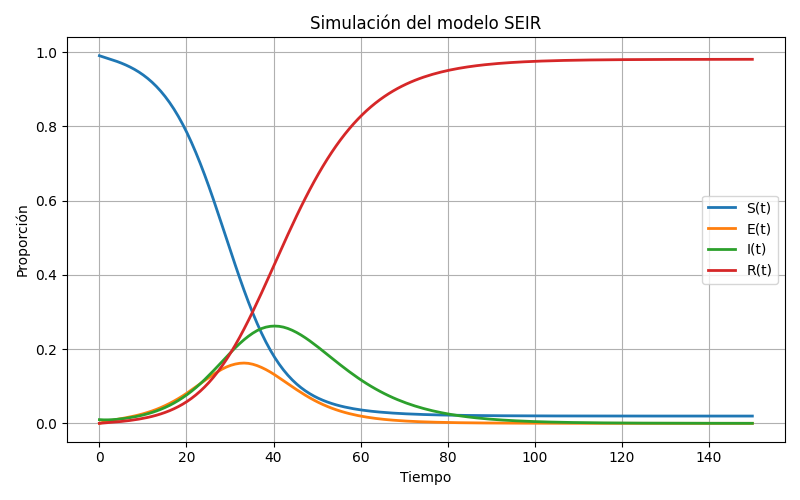
\includegraphics[width=0.7\textwidth]{Graphics/seir_sin_ruido.png}
    \caption{Datos simulados del modelo SEIR}
    \label{fig:seir_sin_ruido}
\end{figure}

El algoritmo se ejecutó con los parámetros de 30 para la población inicial y 20 el número de generaciones.

Los resultados obtenidos durante las 30 ejecuciones del algoritmo genético sobre los datos generados por el modelo SEIR se resumen en la Tabla~\ref{tab:resumen-seir}. En ella se presentan las combinaciones evaluadas según diferentes niveles de ruido en los datos simulados (5\,\%, 15\,\% y 30\,\%) y los valores del parámetro \textit{threshold} (0.8 y 1.0) que determina el criterio de significancia para incluir términos en las ecuaciones diferenciales. Para cada configuración se reporta el mejor valor de \textit{fitness}, el error cuadrático medio (MSE) de validación, y la estructura del grafo inferido que representa las interacciones entre compartimentos.

\begin{table}[H]
\centering
\caption{Resumen de las mejores soluciones para el modelo SEIR bajo distintas configuraciones}
\label{tab:resumen-seir}
\begin{tabular}{|c|c|c|c|c|}
\hline
\textbf{Ruido} & \textbf{\textit{Threshold}} & \textbf{Fitness} & \textbf{MSE Validación} & \textbf{Aristas del Grafo} \\
\hline
5\% & 0.8 & 0.00992 & 0.00586 & 0$\rightarrow$1, 0$\rightarrow$2, 1$\rightarrow$3, 2$\rightarrow$1, 2$\rightarrow$3 \\
5\% & 1.0 & 0.00214 & 0.00123 & 0$\rightarrow$1, 0$\rightarrow$2, 0$\rightarrow$3, 1$\rightarrow$2, 1$\rightarrow$3, 2$\rightarrow$3 \\
15\% & 0.8 & 0.07986 & 0.06807 & 0$\rightarrow$1, 0$\rightarrow$2, 1$\rightarrow$3, 3$\rightarrow$2 \\
15\% & 1.0 & 0.59052 & 0.43875 & 0$\rightarrow$1, 0$\rightarrow$2, 0$\rightarrow$3, 1$\rightarrow$2, 1$\rightarrow$3, 3$\rightarrow$1 \\
30\% & 0.8 & 2.75540 & 0.06372 & 0$\rightarrow$3, 1$\rightarrow$0, 1$\rightarrow$2, 1$\rightarrow$3, 2$\rightarrow$0, 2$\rightarrow$3 \\
30\% & 1.0 & 2.49779 & 0.03656 & 0$\rightarrow$2, 0$\rightarrow$3, 3$\rightarrow$1 \\
\hline
\end{tabular}
\end{table}

\noindent
Para ilustrar los resultados obtenidos, se detallan a continuación las ecuaciones diferenciales correspondientes a algunas de las mejores soluciones halladas. Por ejemplo, en el caso de 5\,\% de ruido y \textit{threshold} de 1.0, la mejor solución obtenida muestra un ajuste muy preciso a los datos originales, con un error cuadrático medio de validación (MSE) de apenas 0.00123. El sistema inferido fue el siguiente:

\[
\begin{aligned}
\frac{dS}{dt} &= -0.40133\,SI - 0.00497\,IR, \\
\frac{dE}{dt} &= 0.19467\,SI - 0.45074\,EI - 0.01597\,IR, \\
\frac{I}{dt} &= 0.12123\,SI + 0.16135\,EI - 0.09800\,IR, \\
\frac{dR}{dt} &= 0.08543\,SI + 0.28939\,EI + 0.11895\,IR.
\end{aligned}
\]

\begin{figure}[H]
\centering
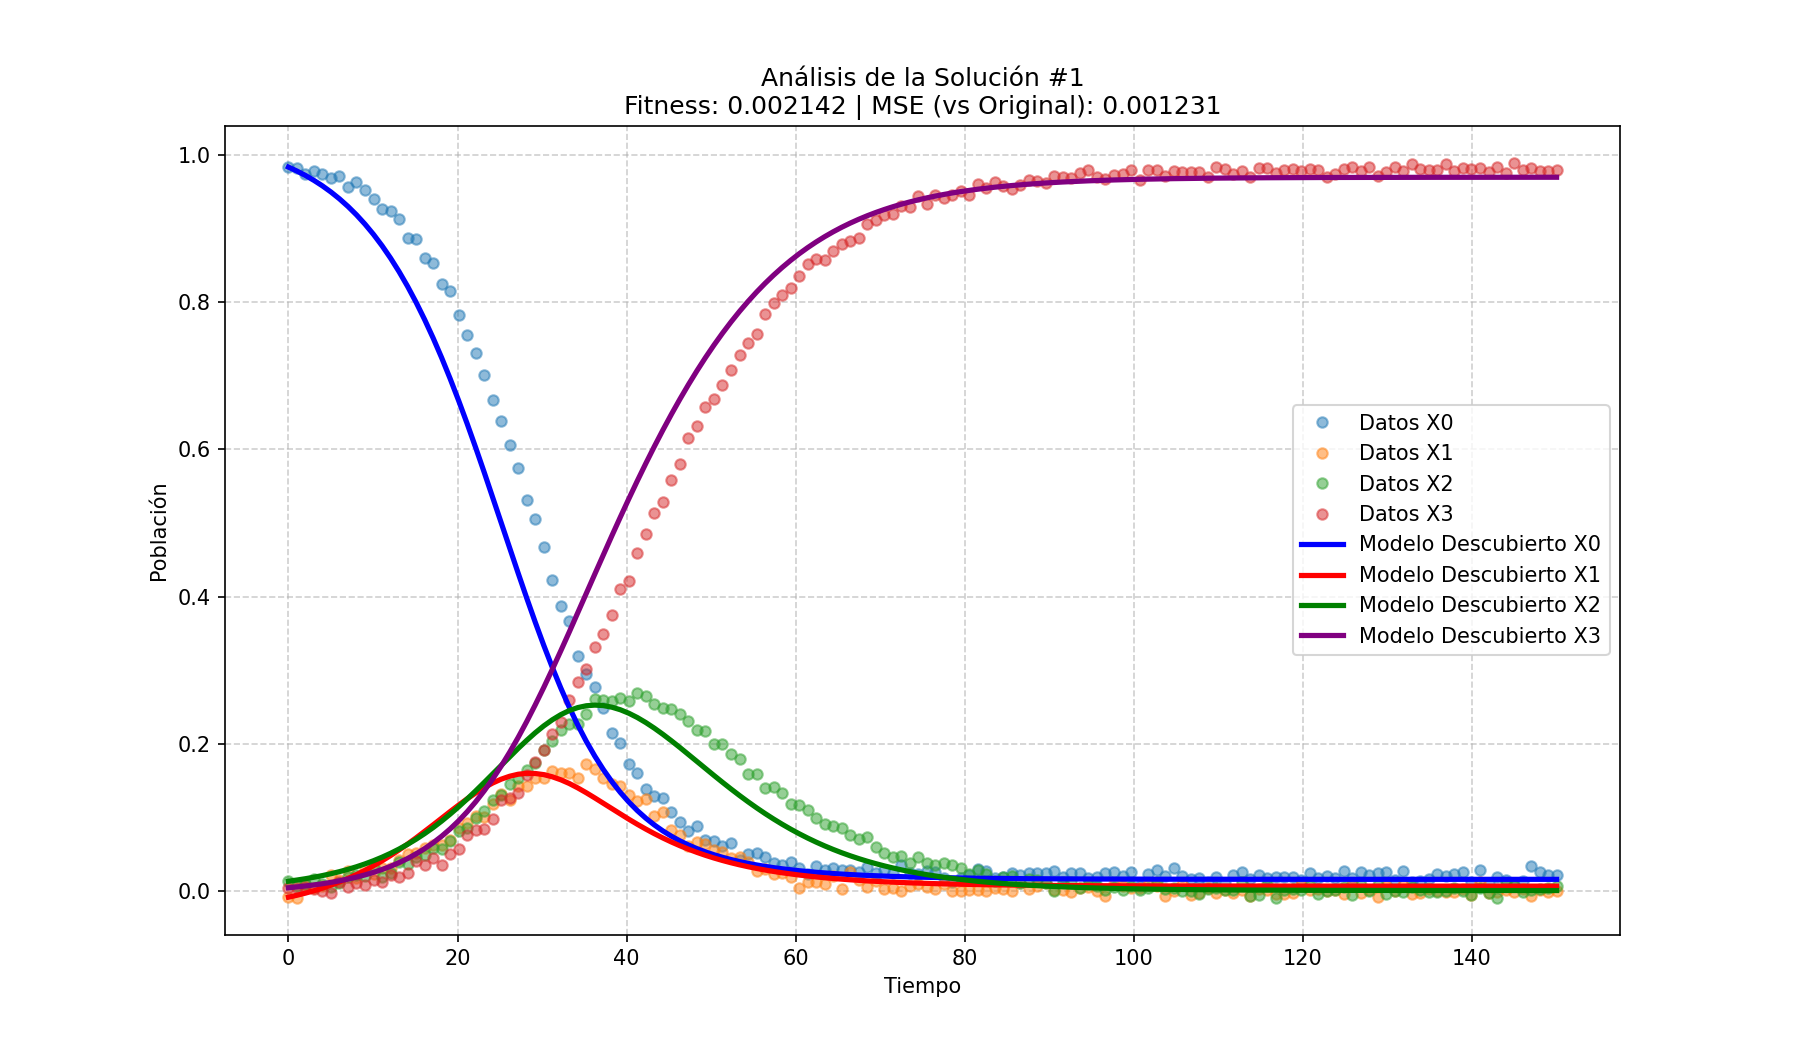
\includegraphics[width=0.7\textwidth]{Graphics/SEIR_noise_0p005_1.0_exp19__solution_1.png}
\caption{Simulación del modelo vs datos reales para 5\% de ruido, \textit{threshold} 1.0. $X_0=S$, $X_1=E$, $X_2=I$, $X_3=R$}
\label{fig:seir_5p_th10}
\end{figure}

En la Figura~\ref{fig:seir_5p_th10} se observa la excelente concordancia entre los datos generados y la simulación del modelo, incluso considerando el pequeño nivel de ruido.

Es interesante destacar que, si bien el sistema con menor \textit{fitness} fue seleccionado como la mejor solución por el algoritmo genético según su función de evaluación, la segunda mejor solución muestra un comportamiento ligeraemente más ajustado a los datos reales. En particular, esta segunda solución presenta un error cuadrático medio (MSE) de validación de apenas 0.001073, valor inferior al reportado por la mejor solución en términos de \textit{fitness}.

Este fenómeno refleja una importante distinción entre el valor de \textit{fitness} utilizado durante la evolución que incluye penalizaciones estructurales y el ajuste puro de los datos medido por el MSE. En este caso en particular la segunda mejor soluci\'on que esta mas ajustadas a los datos tiene una arista m\'as con respecto a la mejor soluci\'on calculada por la funci\'on fitness. 

La solución en cuestión genera el siguiente sistema de ecuaciones diferenciales:
\[
\begin{aligned}
\frac{dS}{dt} &= -0.31590\,SI - 6.93e-17\,IR, \\
\frac{dE}{dt} &= 0.19467\,SI - 0.45074\,EI - 0.01597\,IR, \\
\frac{I}{dt} &= 0.12123\,SI + 0.16135\,EI - 0.09800\,IR, \\
\frac{dR}{dt} &= -1.52e-16\,SI + 0.28939\,EI + 0.11895\,IR.
\end{aligned}
\]
Como se puede observar, aunque el modelo incluye algunos términos de orden muy pequeño, su desempeño en la simulación es altamente preciso. Esto se refleja en la Figura~\ref{fig:seir_5p_th10_sol2}, donde se comparan los datos observados con los obtenidos mediante la integración del sistema inferido.


\begin{figure}[H]
\centering
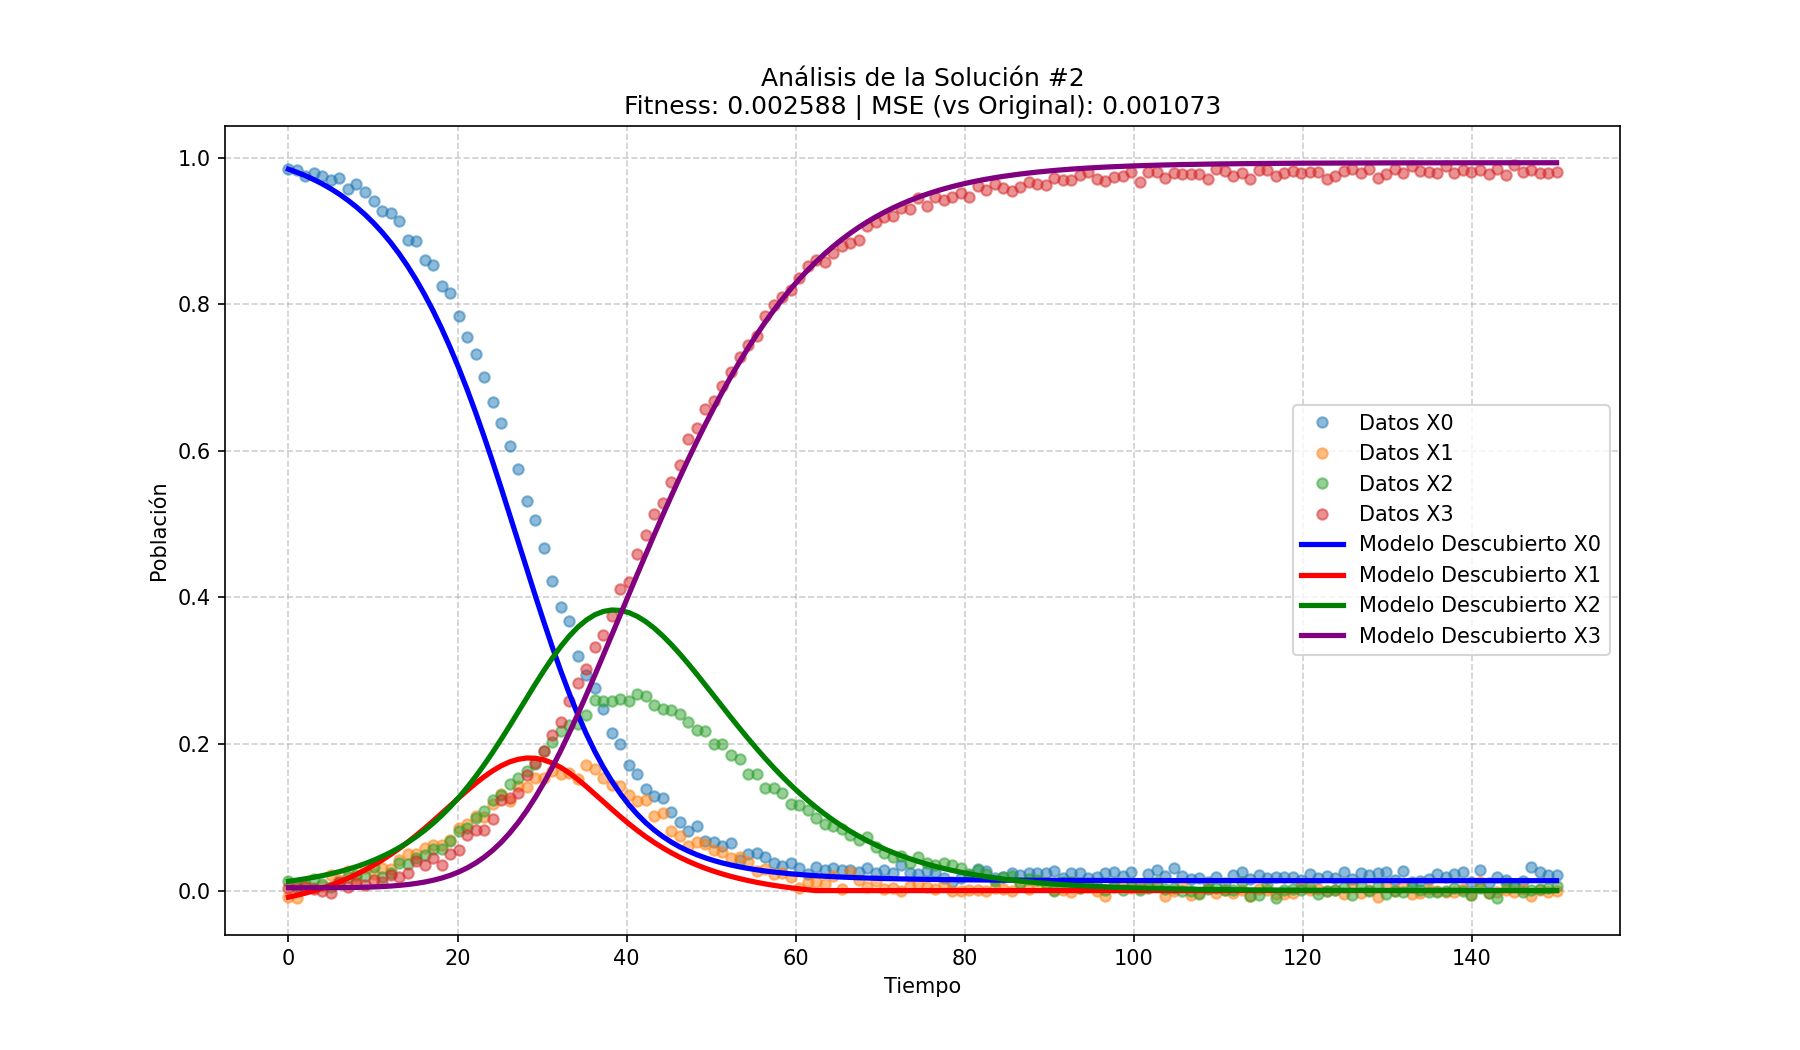
\includegraphics[width=0.7\textwidth]{Graphics/SEIR_noise_0p005_1.0_exp19__solution_2.png}
\caption{Simulación del modelo vs datos reales para 5\% de ruido, \textit{threshold} 1.0. $X_0=S$, $X_1=E$, $X_2=I$, $X_3=R$}
\label{fig:seir_5p_th10_sol2}
\end{figure}

Por otro lado, para niveles de ruido más elevados como el 30\,\%, se logran también resultados destacables. La mejor solución obtenida con \textit{threshold} de 1.0 alcanzó un error de validación de solo 0.03656, lo cual es notable dada la magnitud del ruido incorporado. El sistema inferido en este caso fue:

\[
\begin{aligned}
\frac{dS}{dt} &= -0.01150\,SI - 0.28478\,SR, \\
\frac{dE}{dt} &= 0.23812\,EI, \\
\frac{dI}{dt} &= 0.01150\,SI, \\
\frac{dR}{dt} &= 0.28478\,SR - 0.23812\,EI.
\end{aligned}
\]

\begin{figure}[H]
\centering
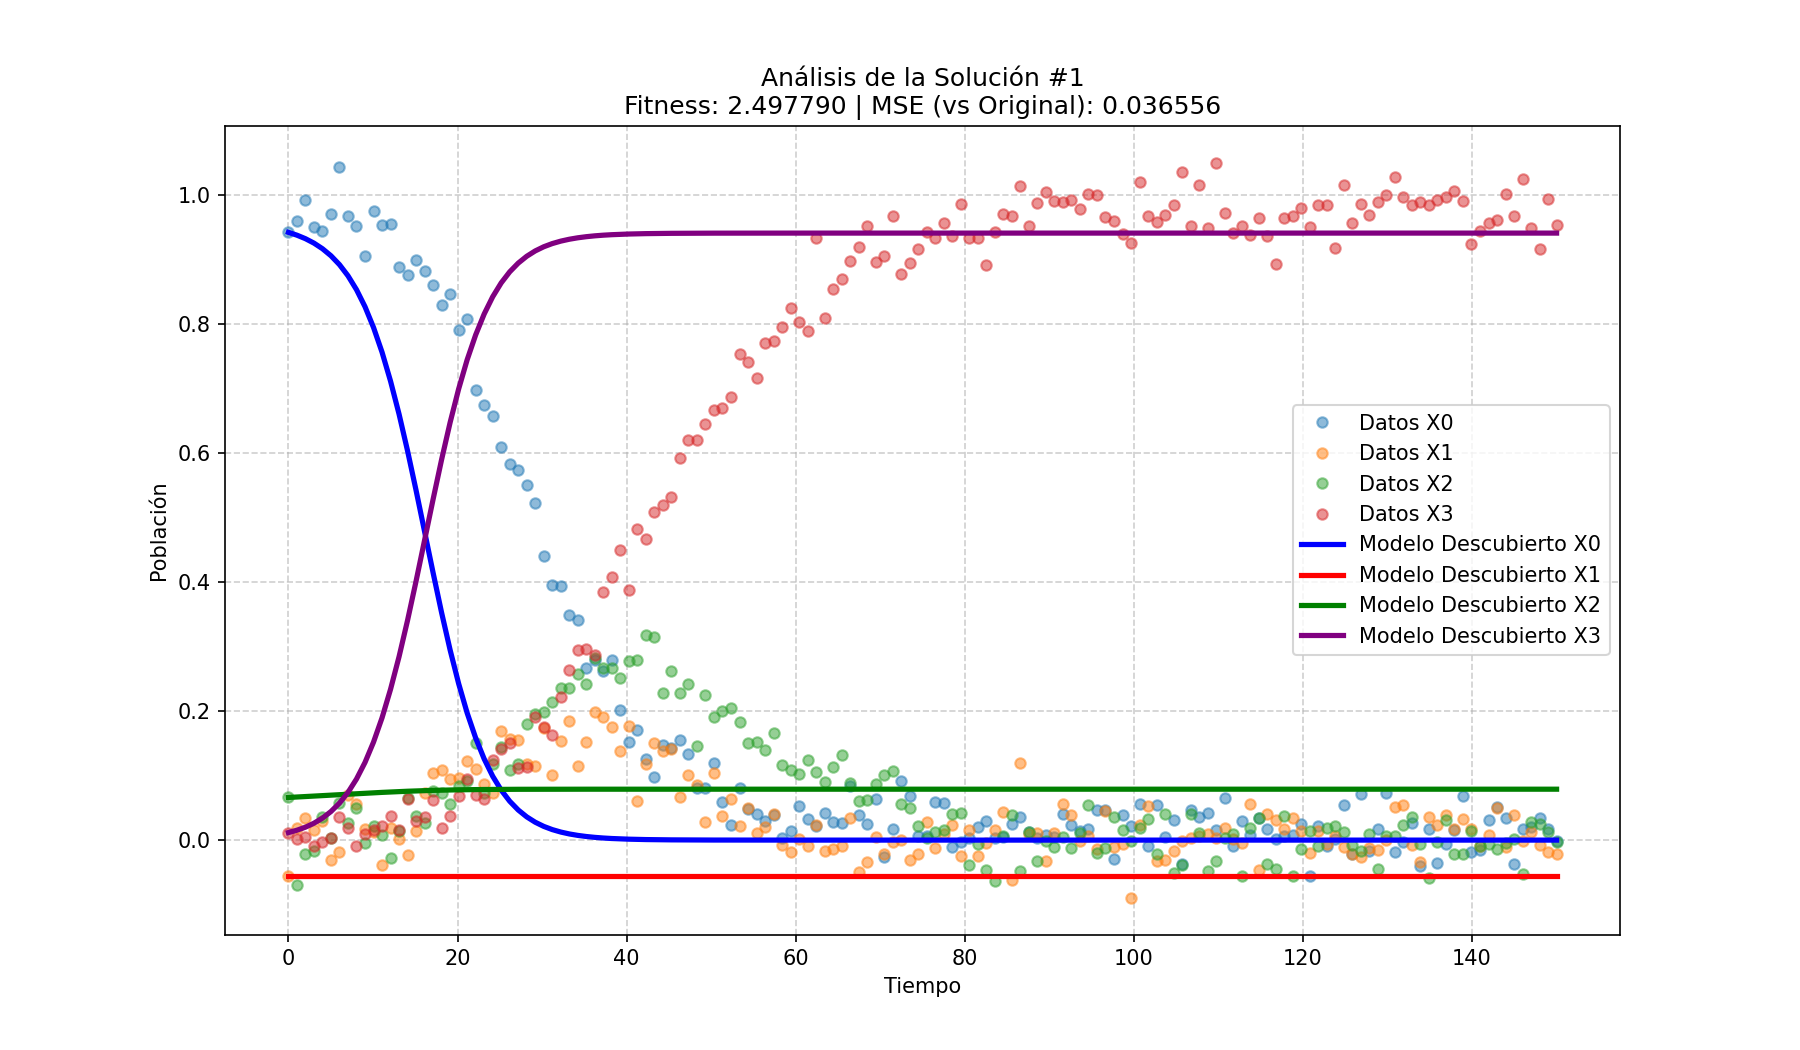
\includegraphics[width=0.7\textwidth]{Graphics/SEIR_noise_0p03_1.0_exp1__solution_1.png}
\caption{Simulación del modelo vs datos reales para 30\% de ruido, \textit{threshold} 1.0. $X_0=S$, $X_1=E$, $X_2=I$, $X_3=R$}
\label{fig:seir_30p_th10}
\end{figure}

A pesar del nivel de ruido, la forma del sistema se mantiene coherente con la estructura compartimental del modelo SEIR, recuperando de manera parcial la dinámica de transición entre compartimentos.

Es importante remarcar que, al igual que en el caso del modelo SIR, no se logró recuperar exactamente la formulación original del modelo generador. Sin embargo, las soluciones inferidas presentan estructuras de grafo razonables y dinámicamente coherentes, ajustándose correctamente a los datos generados, la mejor soluci\'on devuelta contiene todas las aristas del grafo del modelo SEIR. En escenarios con mayor ruido, el algoritmo introduce términos adicionales que probablemente compensan las oscilaciones inducidas por la perturbación estocástica. Aun así, el \textit{fitness} global y los valores de MSE validan la utilidad de las soluciones obtenidas.

Adicionalmente, los tiempos de ejecución promedio del algoritmo genético para cada configuración oscilaron entre los 4 minutos y 24 segundos hasta 5 minutos por experimento. Dependiendo del tamaño de la población, el número de generaciones y la complejidad del grafo inferido estos tiempos son aceptables, considerando la alta dimensionalidad del espacio de búsqueda inducido por todas las posibles configuraciones de grafos válidos y sistemas de ecuaciones asociados.

A continuaci\'on se muestran los resultados de los experimentos del modelo SIRD.


\subsection{Modelo SIRD}

El modelo SIRD es una extensión del clásico modelo SIR y proporciona un marco matemático para analizar la propagación de una enfermedad infecciosa que puede tener un desenlace fatal \cite{Hethcote2000}. El sistema se define mediante el siguiente conjunto de ecuaciones diferenciales:
%
\[
\begin{aligned}
    \frac{dS}{dt} &= -\frac{\beta SI}{S+I+R} , \\
    \frac{dI}{dt} &= \frac{\beta SI}{S+I+R} - \gamma I - \mu I, \\
    \frac{dR}{dt} &= \gamma I, \\
    \frac{dD}{dt} &= \mu I.
\end{aligned}
\]
%
Donde S representa la proporción de individuos susceptibles, I los infecciosos, R los recuperados (y con inmunidad), y D los fallecidos a causa de la enfermedad. El parámetro $\beta$ controla la tasa de transmisión, $\gamma$ es la tasa de recuperación, y $\mu$ representa la tasa de mortalidad del agente infeccioso.

El grafo que representa este sistema está compuesto por las siguientes aristas, que ilustran las transiciones posibles entre los compartimentos: $S \rightarrow I$, $I \rightarrow R$, y $I \rightarrow D$.

Se utilizaron como valores de los parámetros $\beta = 0.5$, $\gamma = 0.1$ y $\mu=0.2$ con punto inicial (0.7, 0.3, 0, 0) y se integró en el intervalo $0 \leq t \leq 150$ para obtener los datos que aparecen en la imagen~\ref{fig:sird_sin_ruido}. Del conjunto de puntos se seleccionaron 150 muestras como datos para el algoritmo gen\'etico. 

\begin{figure}[H]
\centering
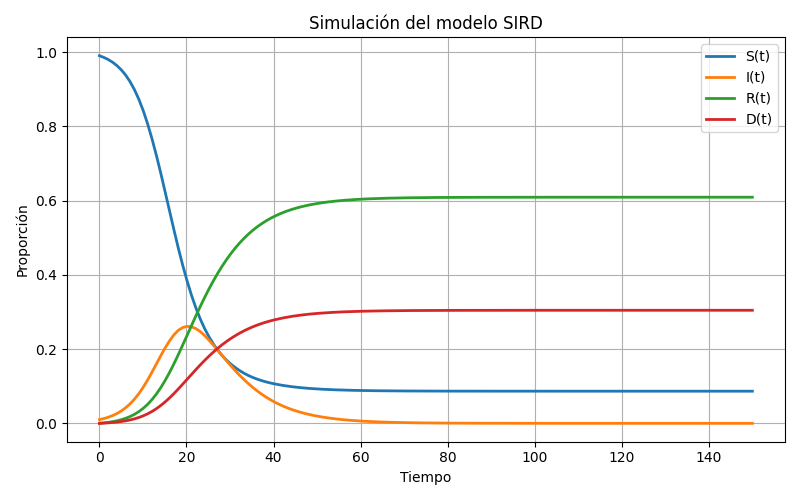
\includegraphics[width=0.7\textwidth]{Graphics/sird_sin_ruido.png}
\caption{Datos simulados del modelo SIRD}
\label{fig:sird_sin_ruido}
\end{figure}

El algoritmo genético fue aplicado usando una población inicial de 30 individuos y 20 generaciones, considerando distintas configuraciones de ruido \( 5\%, 15\%, 30\% \) y valores de \textit{threshold} (0.8 y 1.0). Los resultados obtenidos se resumen en la Tabla~\ref{tab:resumen-sird}.

\begin{table}[H]
\centering
\caption{Resultados experimentales del modelo SIRD bajo diferentes configuraciones}
\label{tab:resumen-sird}
\begin{tabular}{|c|c|c|c|c|}
\hline
\textbf{Ruido} & \textbf{Threshold} & \textbf{MSE Validación} & \textbf{Fitness} & \textbf{Aristas del Grafo} \\
\hline
5\% & 0.8 & 0.171315 & 0.189132 & 0$\rightarrow$2, 1$\rightarrow$2, 2$\rightarrow$1, 3$\rightarrow$2\\
5\% & 1.0 & 0.193155 & 0.210042 & 0$\rightarrow$2, 1$\rightarrow$2, 2$\rightarrow$1, 2$\rightarrow$3\\
15\% & 0.8 & 0.327456 & 0.372651 & 0$\rightarrow$2, 0$\rightarrow$3, 1$\rightarrow$3\\
15\% & 1.0 & 0.060112 & 0.024381 & 0$\rightarrow$1, 1$\rightarrow$2, 2$\rightarrow$3\\
30\% & 0.8 & 0.322215 & 2.323537 & 0$\rightarrow$1, 0$\rightarrow$2, 0$\rightarrow$3\\
30\% & 1.0 & 0.322215 & 2.323537 & 0$\rightarrow$2, 1$\rightarrow$2, 2$\rightarrow$3\\
\hline
\end{tabular}
\end{table}

% Se observa que configuraciones con menor nivel de ruido (5\%) generan resultados consistentes con errores relativamente bajos. En particular, con ruido del 5\% y \textit{threshold} de 0.8 se obtuvo el mejor desempeño relativo a las otras configuraciones con el mismo nivel de ruido. Al aumentar el ruido hasta el 15\%, la configuración con \textit{threshold} de 1.0 mostró un desempeño significativamente mejor en términos de fitness (0.024381) y MSE (0.060112) respecto al caso con \textit{threshold} de 0.8.

A continuación se detallan las ecuaciones diferenciales correspondientes a una de las mejores soluciones obtenidas en los experimentos, específicamente con un nivel de ruido del 15\% y un \textit{threshold} de 1.0. Esta configuración destacó notablemente por lograr un ajuste preciso a los datos experimentales (de manera consistente en los 30 experimentos), reflejado en un bajo valor de MSE (0.060112) y excelente valor de \textit{fitness} (0.024381). El sistema inferido en este caso es:

\[
\begin{aligned}
\frac{dS}{dt} &= -0.34662\,S I, \\
\frac{dI}{dt} &= 0.34662\,S I - 0.23721\,I R, \\
\frac{dR}{dt} &= -0.24310\,S D + 0.23721\,I R - 1.19084\,I D - 1.83079\,R D - 2.97057\,D^2 - 0.85770\,D, \\
\frac{dD}{dt} &= 0.24310\,S D + 1.19084\,I D + 1.83079\,R D + 2.97057\,D^2 + 0.85770\,D.
\end{aligned}
\]

\begin{figure}[H]
\centering
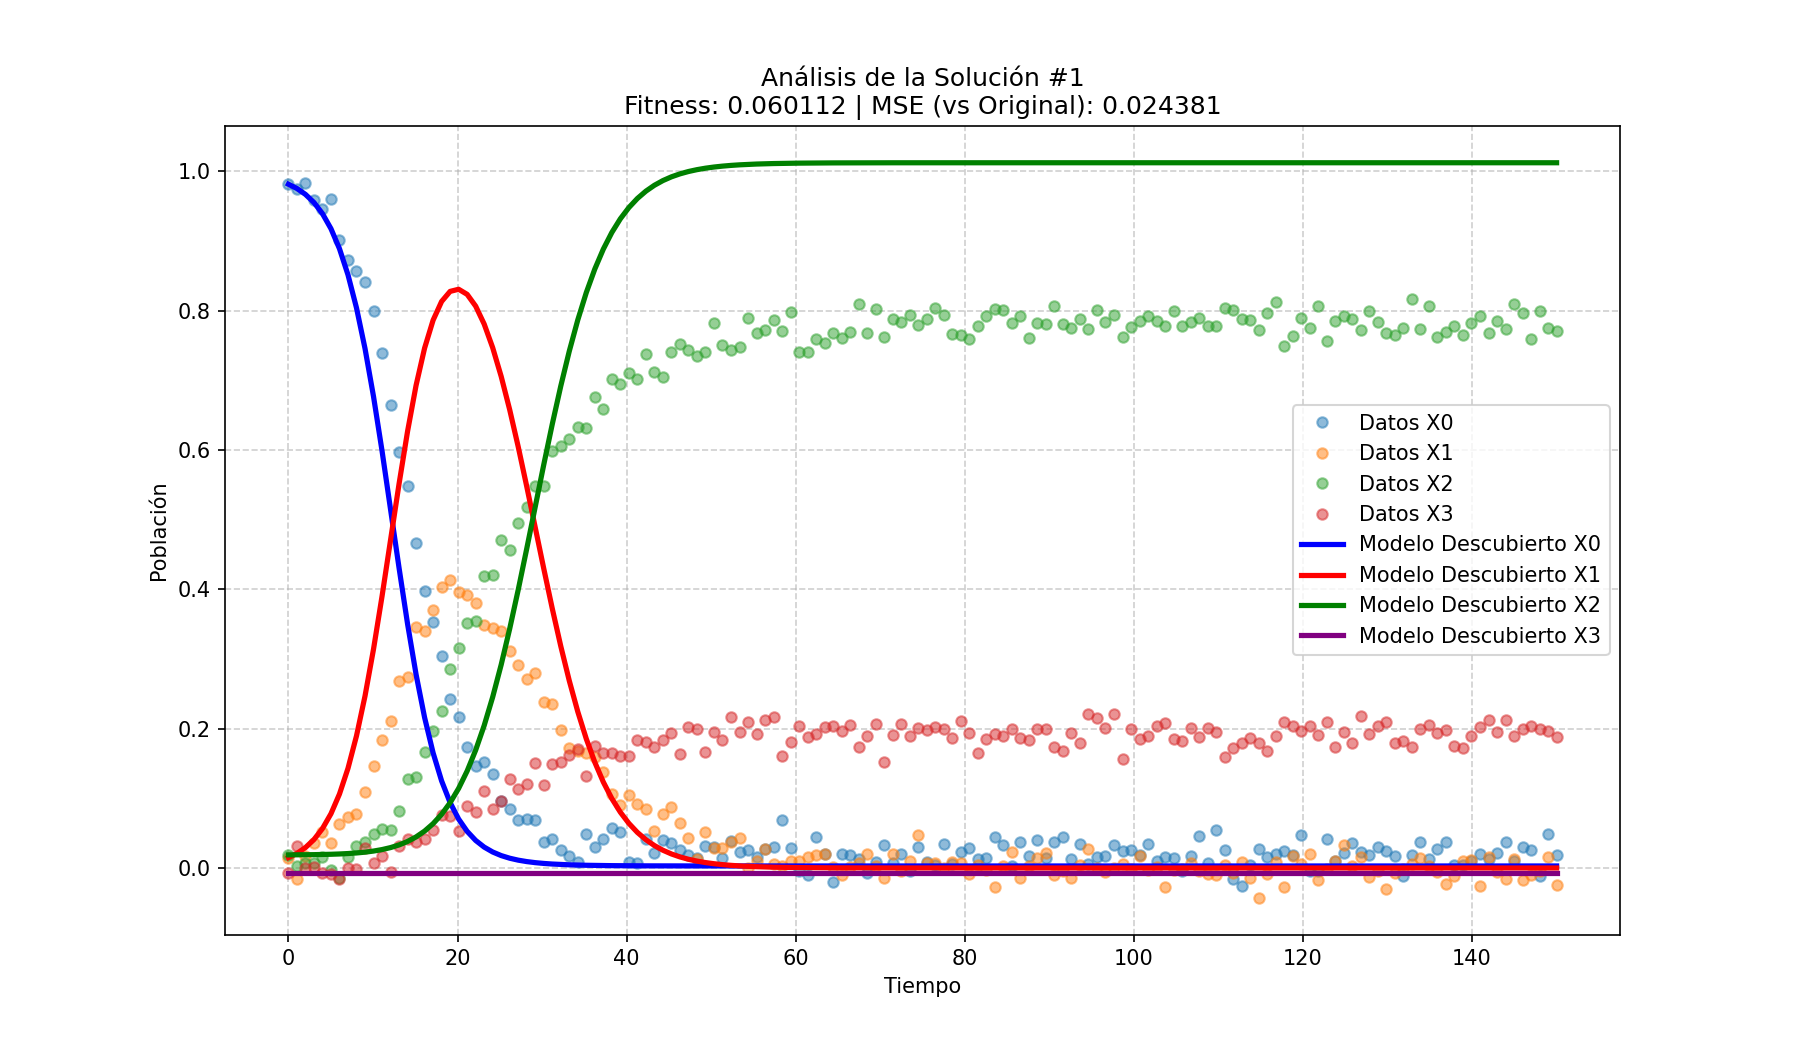
\includegraphics[width=0.7\textwidth]{Graphics/SIRD_noise_0p015_1.0_exp1__solution_1.png}
\caption{Simulación del modelo vs datos reales para 15\% de ruido, \textit{threshold} 1.0. $X_0=S$, $X_1=I$, $X_2=R$, $X_3=D$}
\label{fig:sird_15p_th10}
\end{figure}

Estos resultados muestran cómo, pese al ruido considerable presente en los datos, el algoritmo logró identificar correctamente relaciones significativas entre los compartimentos del modelo SIRD. Se observa, sin embargo, la introducción de términos adicionales respecto al modelo original, que indican mecanismos compensatorios del modelo frente a la perturbación del ruido. Se puede observar en la Figura~\ref{fig:sird_15p_th10} la cercania entre los datos generados y la soluci\'on encontrada.

Sin embargo, las soluciones halladas con otras configuraciones de par\'ametros (ruido y threshold), no se ajustan muy bien a los datos, y al alcanzar niveles altos de ruido (30\%), el desempeño del modelo inferido decae sustancialmente, reflejado en un incremento significativo del valor del fitness y del MSE, indicando dificultad para capturar las dinámicas originales del modelo SIRD con alta perturbación en los datos.

Se presenta el segundo conjunto de soluciones que mejor se ajustan a los datos, correspondientes al escenario con un 5\% de ruido y \textit{threshold} de 0.8. Aunque esta solución obtuvo valores considerablemente superiores en términos de error cuadrático medio (MSE de 0.171315) y \textit{fitness} (0.189132), sigue siendo relevante para entender la variabilidad de los resultados inferidos respecto al nivel de ruido. Las ecuaciones diferenciales inferidas en este caso son:

$$
\begin{aligned}
\frac{dS}{dt} &= -0.29877\,S I - 0.02877\,I R - 0.04429\,R^2 - 0.18030\,R D, \\
\frac{dI}{dt} &= 4.73 \times 10^{-15}\,I R - 8.33 \times 10^{-17}ID\, - 7.69 \times 10^{-15}\,R^2\, - 1.71 \times 10^{-15} R D, \\
\frac{dR}{dt} &= 0.29877\,S I + 0.02877\,I R + 0.73276\,I D + 0.04429\,R^2 + 0.18030\,R D + 3.69095\,D^2 + 0.72146\,D, \\
\frac{dD}{dt} &= -0.73276\,I D - 3.69095\,D^2 - 0.72146\,D.
\end{aligned}
$$

\begin{figure}[H]
\centering
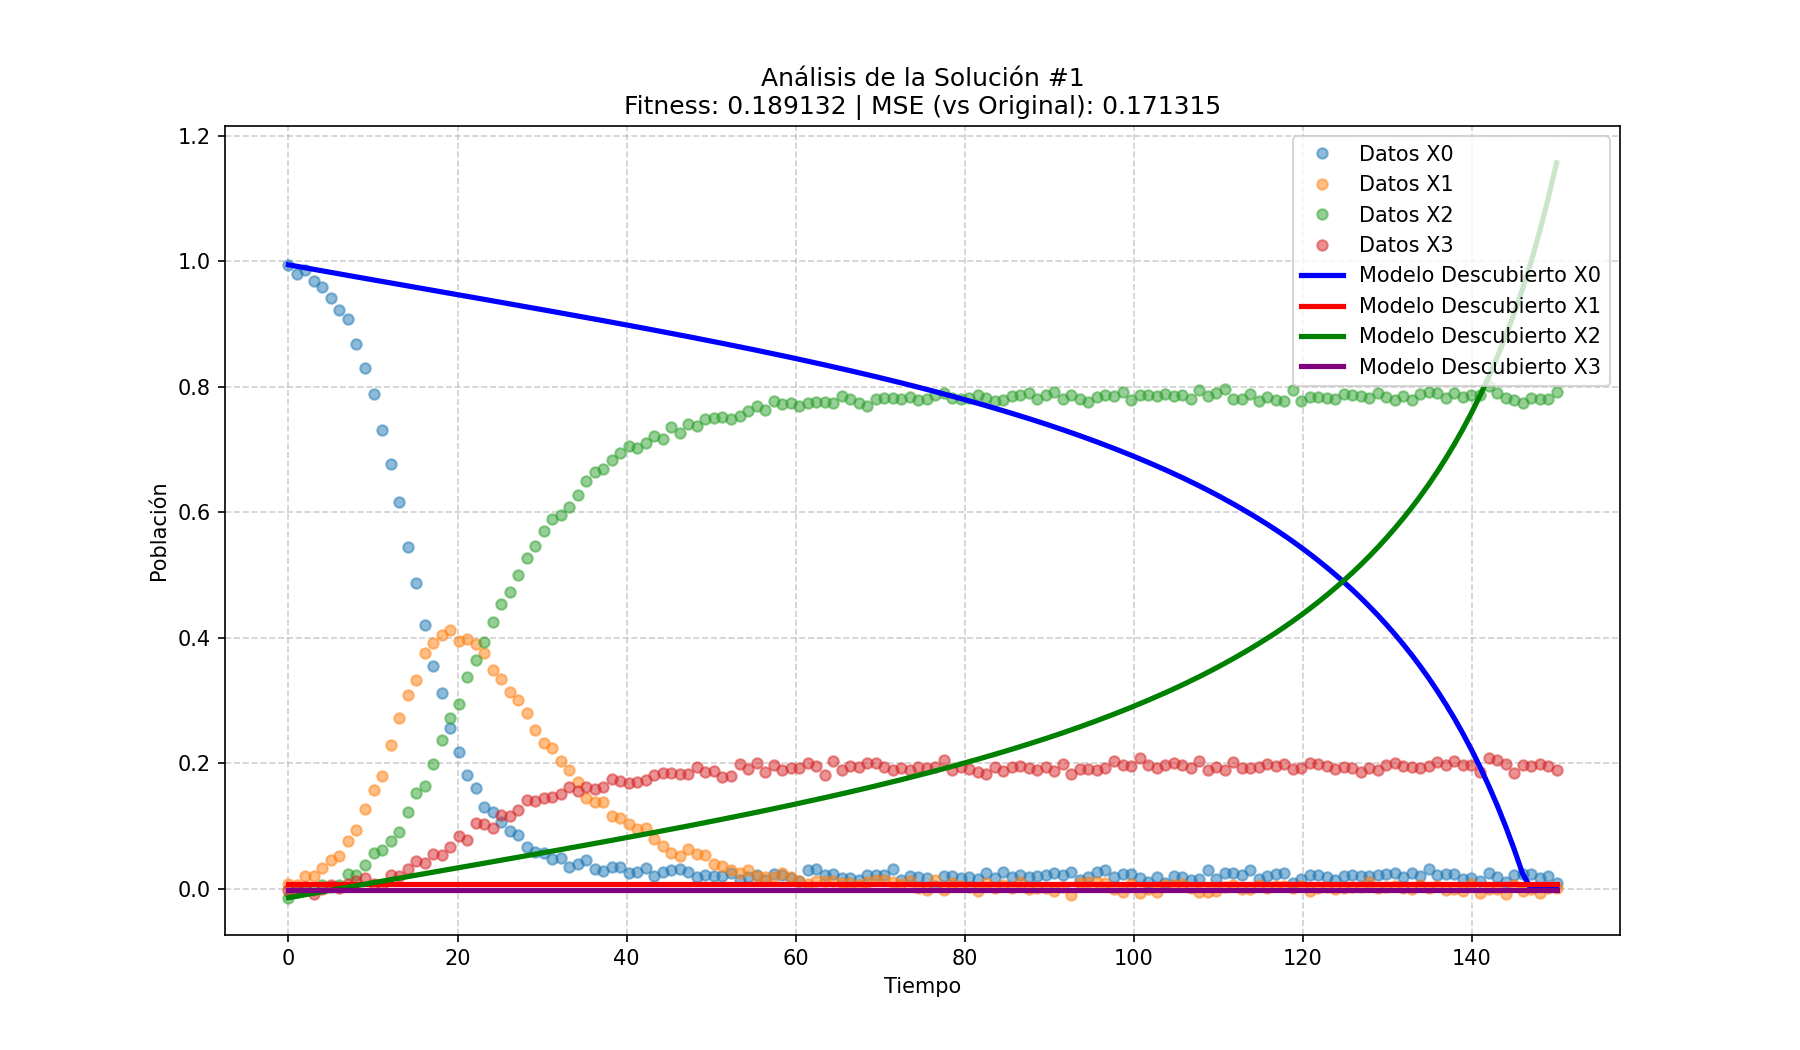
\includegraphics[width=0.7\textwidth]{Graphics/SIRD_noise_0p005_0.8_exp1__solution_1.png}
\caption{Simulación del modelo vs datos reales para 15\% de ruido, \textit{threshold} 1.0. $X_0=S$, $X_1=I$, $X_2=R$, $X_3=D$}
\label{fig:sird_5p_th08}
\end{figure}

La Figura~\ref{fig:sird_5p_th08} muestra gráficamente la simulación del modelo inferido en comparación con los datos originales generados bajo estas condiciones experimentales.

En esta figura se observa claramente que, aunque el modelo capturó parcialmente las tendencias generales, presenta mayores desviaciones respecto a los datos originales en comparación con la mejor solución previamente analizada. Esto subraya la importancia crítica del nivel de ruido y el \textit{threshold} elegido para obtener modelos más precisos y robustos.

En términos de rendimiento computacional, el tiempo requerido para cada ejecución del algoritmo genético se mantuvo en un rango de 3 minutos y 48 segundos a 4 minutos y 53 segundos. Este rendimiento se considera razonable dada la carga computacional que imponen un sistema con cuatro compartimentos.

En la proxima secci\'on se exponen los resultados de la experimentaci\'on con el modelo SEIRV.

\subsection{Modelo SEIRV}

El modelo SEIRV amplía el marco del modelo SEIR para incluir el efecto de las campañas de vacunación en la dinámica de una enfermedad. Este enfoque proporciona una herramienta matemática para evaluar cómo la inmunización interviene en la propagación de una infección que posee un período de latencia \cite{Anderson1991}. El sistema se define mediante el siguiente conjunto de ecuaciones diferenciales:

\[
\begin{aligned}
    \frac{dS}{dt} &= -\frac{\beta SI}{N} - \nu S, \\
    \frac{dE}{dt} &= \frac{\beta SI}{N} - \alpha E, \\
    \frac{dI}{dt} &= \alpha E - \gamma I, \\
    \frac{dR}{dt} &= \gamma I, \\
    \frac{dV}{dt} &= \nu S.
\end{aligned}
\]

Donde $N = S+E+I+R+V$. Las variables representan la proporción de individuos: \textbf{S} (susceptibles), \textbf{E} (expuestos, en período de incubación), \textbf{I} (infecciosos), \textbf{R} (recuperados) y \textbf{V} (vacunados). Los parámetros del modelo son: $\beta$ para la tasa de transmisión, $\alpha$ la tasa de progresión de expuesto a infeccioso, $\gamma$ la tasa de recuperación, y $\nu$ la tasa de vacunación sobre la población susceptible.

El grafo que representa este sistema está compuesto por las siguientes aristas, que ilustran las transiciones posibles: $S \rightarrow E$, $S \rightarrow V$, $E \rightarrow I$ y $I \rightarrow R$.

Se utilizaron como valores de los parámetros $\beta = 0.5$, $\alpha = 0.2$, $\gamma = 0.1$ y $\nu = 0.05$ con punto inicial (0.9, 0.1, 0, 0, 0) y se integró en el intervalo $0 \leq t \leq 150$ para obtener los datos que aparecen en la Figura~\ref{fig:seirv_sin_ruido}. Del conjunto de puntos se seleccionaron 150 muestras como datos para el algoritmo genético.

\begin{figure}[H]
    \centering
    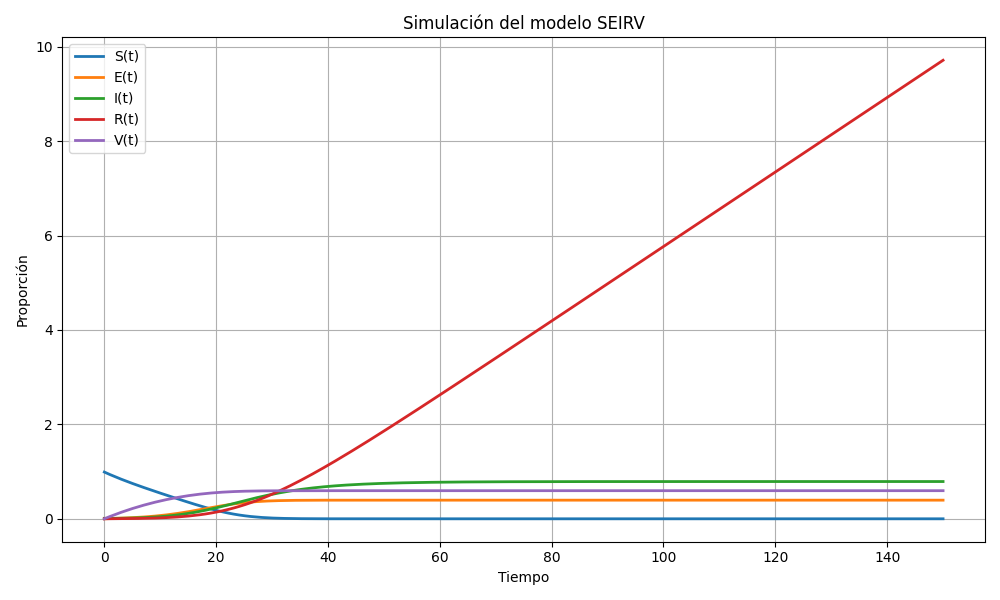
\includegraphics[width=0.7\textwidth]{Graphics/seirv_sin_ruido.png}
    \caption{Datos simulados del modelo SEIRV}
    \label{fig:seirv_sin_ruido}
\end{figure}

El algoritmo genético fue aplicado usando una población inicial de 40 individuos y 40 generaciones, considerando distintas configuraciones de ruido \( 5\%, 15\%, 30\% \) y valores de \textit{threshold} (0.8 y 1.0).Los resultados obtenidos se resumen en la Tabla~\ref{tab:resumen-seirv}.

\begin{table}[H]
\centering
\caption{Resultados experimentales del modelo SEIRV bajo diferentes configuraciones}
\label{tab:resumen-seirv}
\begin{tabular}{|c|c|c|c|c|}
\hline
\textbf{Ruido} & \textbf{Threshold} & \textbf{MSE Validación} & \textbf{Fitness} & \textbf{Aristas del Grafo} \\
\hline
5\% & 0.8 & 3.29928170 & 3.61697174 & 0$\rightarrow$3, 1$\rightarrow$3, 1$\rightarrow$4, 2$\rightarrow$1, 2$\rightarrow$3, 4$\rightarrow$2\\
5\% & 1.0 & 3.70048194 & 3.84277075 & 0$\rightarrow$3, 1$\rightarrow$3, 2$\rightarrow$1, 4$\rightarrow$1, 4$\rightarrow$3\\
15\% & 0.8 & 3.58154992 & 4.08872264 & 0$\rightarrow$2, 0$\rightarrow$4, 2$\rightarrow$3, 4$\rightarrow$1, 4$\rightarrow$2\\
15\% & 1.0 & 3.45445046 & 4.09157519 & 0$\rightarrow$1, 0$\rightarrow$4, 2$\rightarrow$0, 2$\rightarrow$3, 3$\rightarrow$1, 4$\rightarrow$2\\
30\% & 0.8 & 3.97527256 & 4.31880023 & 0$\rightarrow$4, 1$\rightarrow$2, 3$\rightarrow$1, 4$\rightarrow$3\\
30\% & 1.0 & 4.09472754 & 4.47803501 & 0$\rightarrow$1, 0$\rightarrow$3, 1$\rightarrow$2, 1$\rightarrow$3, 2$\rightarrow$4\\
\hline
\end{tabular}
\end{table}

A diferencia de los modelos anteriores, la inferencia del modelo SEIRV presentó una mayor complejidad, reflejada en valores de MSE y \textit{fitness} considerablemente más altos en todas las configuraciones. A continuación, se analizan las mejores soluciones obtenidas para cada nivel de ruido.

Para un nivel de ruido del 5\%, la mejor solución se encontró con un \textit{threshold} de 0.8, obteniendo un MSE de validación de 3.299. El sistema de ecuaciones inferido es el siguiente:
\[
\begin{aligned}
\frac{dS}{dt} &= -0.25372\,S V, \\
\frac{dE}{dt} &= -0.33050\,S E - 0.02951\,S V - 0.79277\,E^2 - 0.63327\,E I + 0.51342\,E, \\
\frac{dI}{dt} &= -3.75503\,S E - 1.80538\,S I - 4.61293\,E^2 - 1.96860\,E I + 2.42742\,E V \\ & \quad - 3.13577\,E - 0.90574\,I V - 1.48401\,I, \\
\frac{dR}{dt} &= 3.70352\,S E + 1.80538\,S I + 0.25372\,S V + 4.24854\,E^2 + 2.58864\,E I \\ & \quad + 1.67204\,E + 0.90574\,I V + 1.48401\,I, \\
\frac{dV}{dt} &= 0.38201\,S E + 0.02951\,S V + 1.15716\,E^2 + 0.01324\,E I - 2.42742\,E V + 0.95030\,E.
\end{aligned}
\]
\begin{figure}[H]
    \centering
    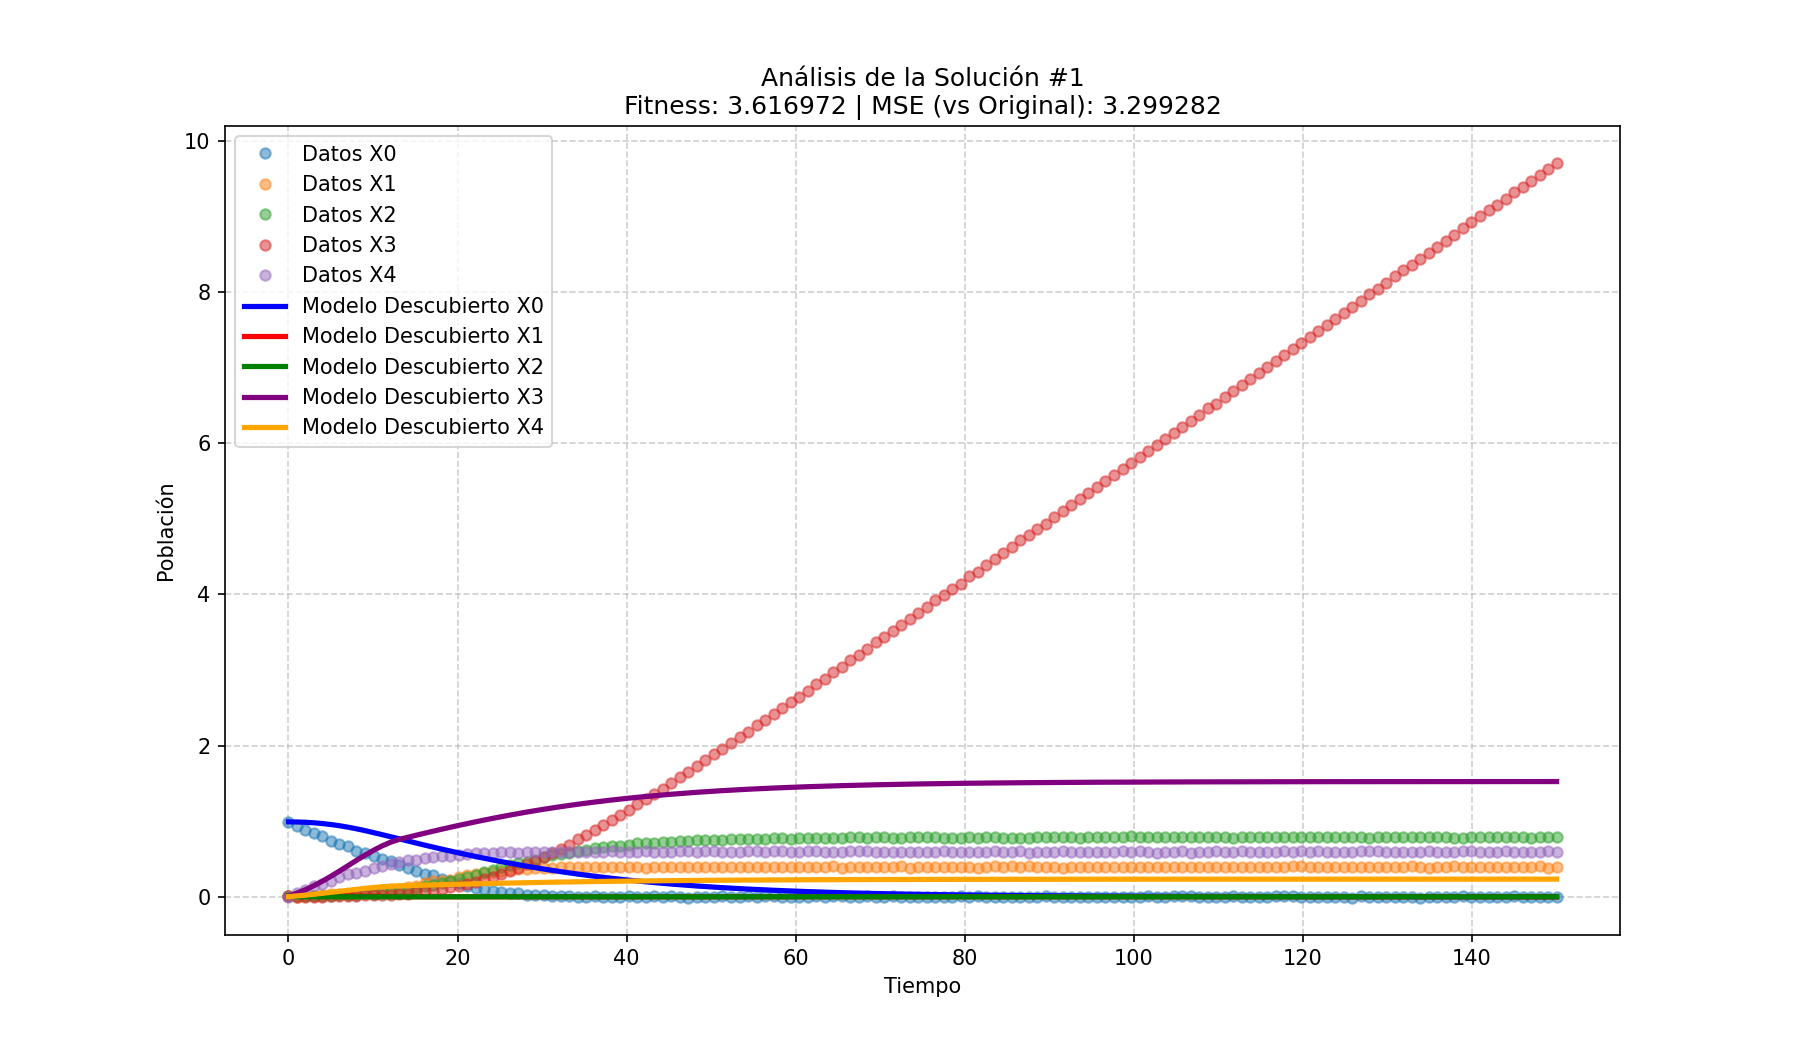
\includegraphics[width=0.7\textwidth]{Graphics/SEIRV_noise_0p005_0.8_exp2__solution_1.png}
    \caption{Simulación del mejor modelo SEIRV vs datos reales para 5\% de ruido, \textit{threshold} 0.8. ($X_0=S, X_1=E, X_2=I, X_3=R, X_4=V$)}
    \label{fig:seirv_5p_th08}
\end{figure}

Al incrementar el ruido al 15\%, el mejor resultado se obtuvo con un \textit{threshold} de 1.0, alcanzando un MSE de validación de 3.454. Este valor, aunque elevado, fue el más bajo para este nivel de ruido. Las ecuaciones inferidas fueron:
\[
\begin{aligned}
\frac{dS}{dt} &= -0.72788\,S E + 0.25454\,S V - 0.03815\,S - 0.78280\,E V - 0.04831\,V^2 - 0.22807\,V, \\
\frac{dE}{dt} &= 0.57364\,S E + 0.03439\,S V + 0.14612\,E V, \\
\frac{dI}{dt} &= -0.13629\,S E - 0.28893\,S V - 0.15875\,E I + 0.57387\,E V + 0.35234\,V^2 + 0.30526\,V, \\
\frac{dR}{dt} &= -0.19364\,S E + 0.23142\,E I - 0.03907\,E V, \\
\frac{dV}{dt} &= 0.48417\,S E + 0.03815\,S - 0.07267\,E I + 0.10188\,E V - 0.30403\,V^2 - 0.07718\,V.
\end{aligned}
\]
\begin{figure}[H]
    \centering
    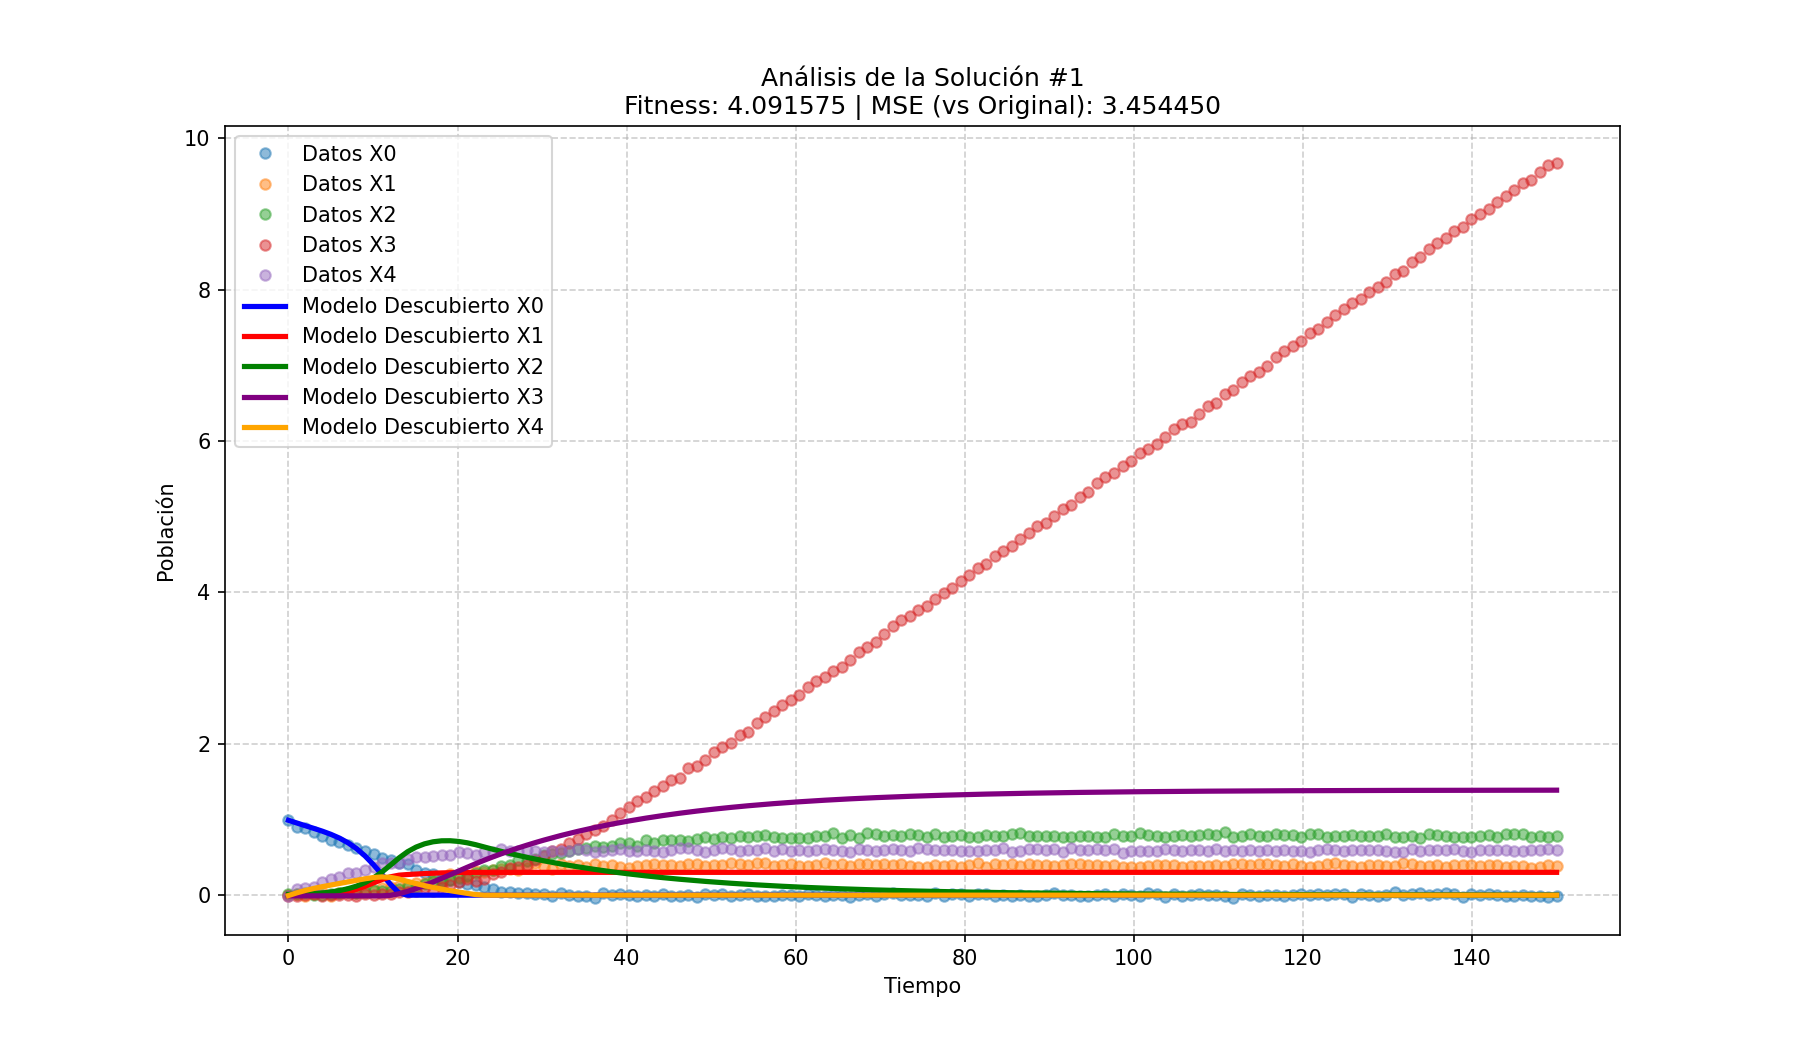
\includegraphics[width=0.7\textwidth]{Graphics/SEIRV_noise_0p015_1.0_exp1__solution_1.png}
    \caption{Simulación del mejor modelo SEIRV vs datos reales para 15\% de ruido, \textit{threshold} 1.0. ($X_0=S, X_1=E, X_2=I, X_3=R, X_4=V$)}
    \label{fig:seirv_15p_th10}
\end{figure}

Finalmente, con un 30\% de ruido, la solución con menor error (MSE de 3.975) volvió a corresponder a un \textit{threshold} de 0.8. El sistema resultante, aunque muy alejado del modelo teórico, representa el mejor ajuste encontrado bajo estas condiciones de alta incertidumbre.
\[
\begin{aligned}
\frac{dS}{dt} &= -0.66931\,S I, \\
\frac{dE}{dt} &= -0.41171\,S E - 0.40749\,S I + 0.20785\,E V + 0.17254\,E, \\
\frac{dI}{dt} &= 0.69568\,S E + 0.40749\,S I + 0.03826\,E, \\
\frac{dR}{dt} &= -0.28397\,S E - 0.16943\,E V - 0.21079\,E + 0.06849\,I V, \\
\frac{dV}{dt} &= 0.66931\,S I - 0.03842\,E V - 0.06849\,I V.
\end{aligned}
\]
\begin{figure}[H]
    \centering
    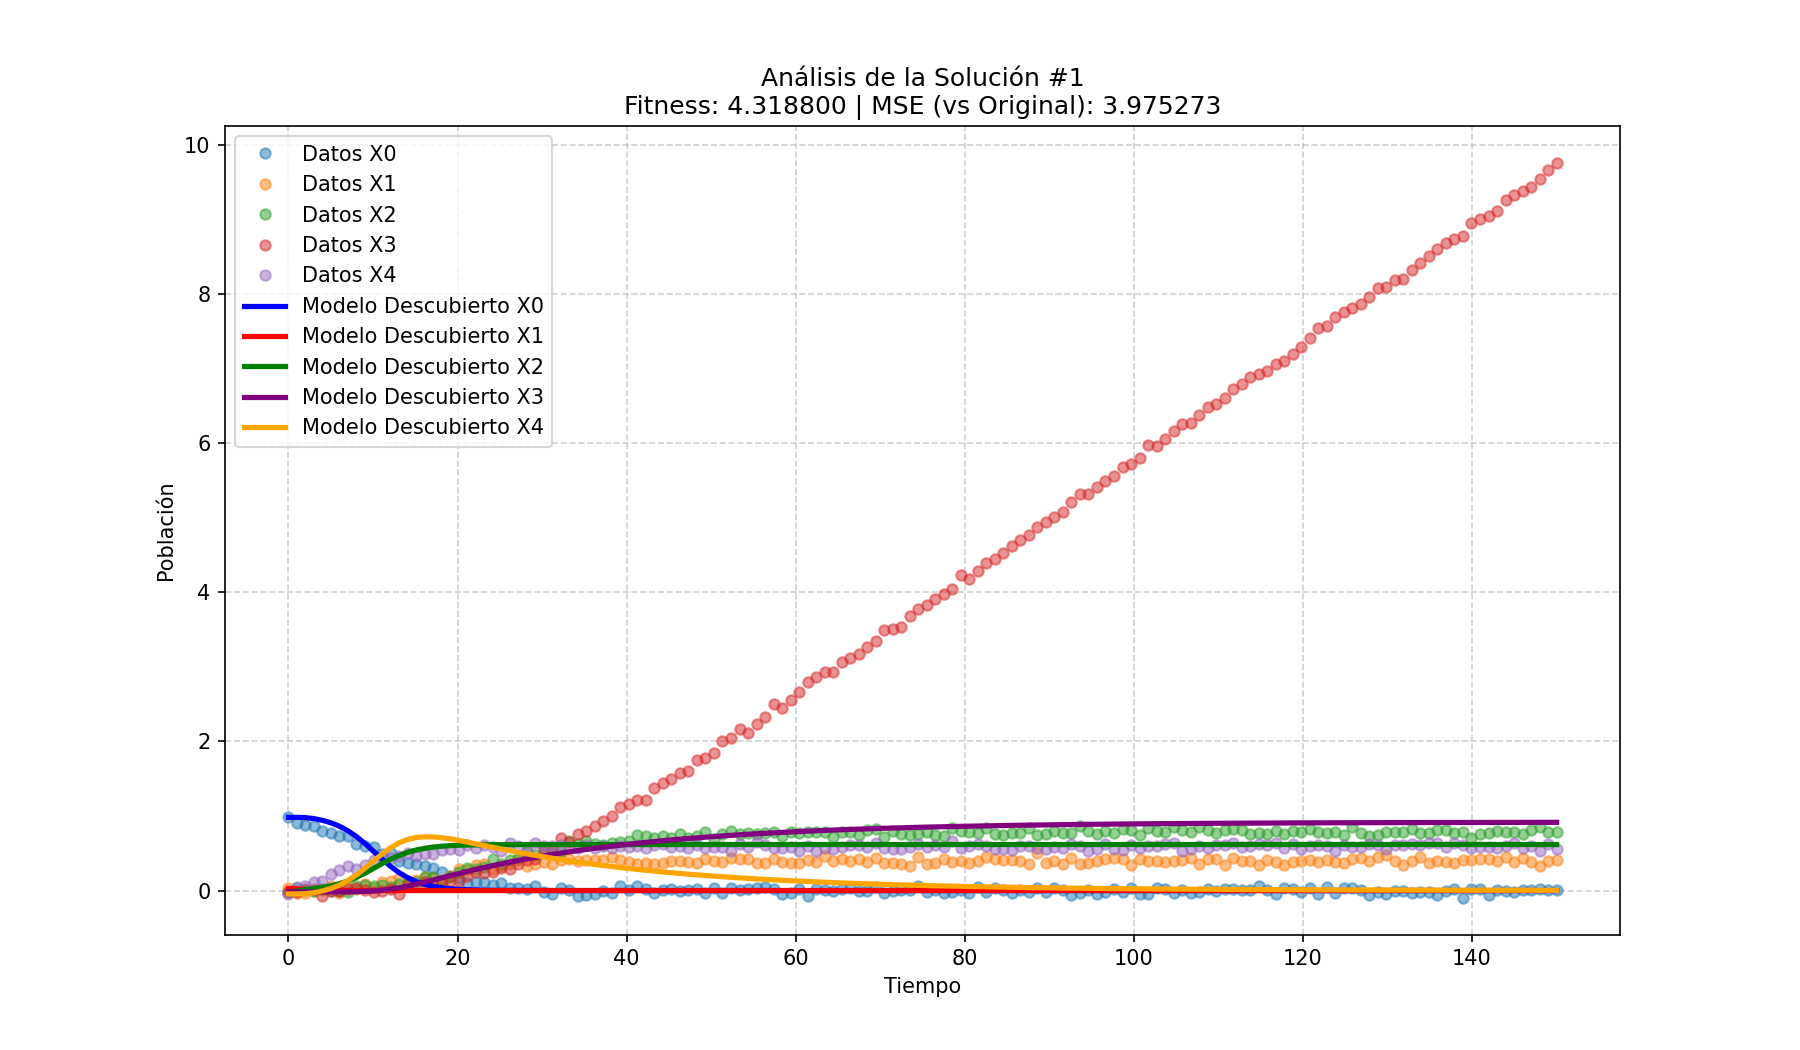
\includegraphics[width=0.7\textwidth]{Graphics/SEIRV_noise_0p03_0.8_exp1__solution_1.png}
    \caption{Simulación del mejor modelo SEIRV vs datos reales para 30\% de ruido, \textit{threshold} 0.8. ($X_0=S, X_1=E, X_2=I, X_3=R, X_4=V$)}
    \label{fig:seirv_30p_th08}
\end{figure}

Adicionalmente, es relevante mencionar los tiempos de ejecución para los experimentos del modelo SEIRV. Dada la mayor complejidad del sistema, con cinco compartimentos, y el aumento en los parámetros del algoritmo genético (40 individuos y 40 generaciones), los tiempos por experimento oscilaron entre 8 minutos y 57 segundos y 10 minutos con 12 segundos.

En resumen, los experimentos con el modelo SEIRV demuestran las limitaciones del método frente a sistemas de mayor dimensionalidad y complejidad. Los valores de MSE obtenidos son significativamente más altos que en los modelos previos, y las estructuras de los grafos y ecuaciones inferidas divergen considerablemente del modelo teórico. Es crucial destacar que los resultados sugieren que no existe una receta exacta o una configuración de parámetros (como el \textit{threshold}) que garantice el mejor resultado de manera consistente. En los casos analizados, las mejores soluciones se alternaron entre un \textit{threshold} de 0.8 y 1.0, lo que indica que la elección óptima de este parámetro depende intrínsecamente del nivel de ruido y de las características específicas de los datos, requiriendo un proceso de ajuste y validación para cada problema particular.

En la siguiente sección se realiza un análisis de los resultados de todos
los experimentos realizados.

\section{An\'alisis de resultados}
\label{sec:experimentation4}

Los experimentos realizados muestran que el algoritmo genético propuesto es capaz de inferir sistemas compartimentales que, aunque no siempre replican exactamente las ecuaciones originales, logran capturar con notable precisión la dinámica subyacente de los datos generados. La metodología basada en grafos dirigidos y ecuaciones polinómicas cuadráticas ajustadas por mínimos cuadrados permite una exploración eficiente del espacio de modelos compartimentales posibles.

En los casos correspondientes a los modelos SIR y SEIR, los resultados obtenidos destacan por su alto grado de fidelidad en la aproximación de las trayectorias observadas, especialmente en escenarios de bajo ruido (5\%). Incluso en estos casos, si bien la estructura original del modelo no fue completamente recuperada en todos los experimentos, las ecuaciones encontradas presentan formas compatibles con la dinámica esperada, y el grafo inferido recupera correctamente las transiciones clave entre compartimentos. Además, los valores del error cuadrático medio (MSE) y del \textit{fitness} alcanzan órdenes de magnitud muy bajos, particularmente en los experimentos con \textit{threshold} 1.0 y niveles de ruido bajos, donde el sistema SEIR obtuvo un MSE tan pequeño como 0.001073.

Cabe resaltar un fenómeno interesante identificado en el modelo SEIR: la solución con menor MSE no fue la seleccionada como la mejor por el algoritmo genético, debido a que el \textit{fitness} penaliza también la complejidad estructural del sistema ,por ejemplo, el número de aristas en el grafo. La segunda mejor solución en términos de \textit{fitness} generó un sistema con una arista adicional, pero ajustó mejor los datos simulados. Este caso pone de manifiesto que la métrica de ajuste (MSE) y la función de evaluación evolutiva (\textit{fitness}) no siempre convergen en la misma solución, lo cual puede ser relevante en aplicaciones donde se prioriza la precisión sobre la simplicidad.

En el modelo SIRD, que introduce términos no lineales con fracciones en su formulación original, los resultados muestran mayor dispersión. Aunque algunas configuraciones experimentales lograron ajustes razonables, por ejemplo, MSE de 0.060112 en el caso con 15\% de ruido y \textit{threshold} 1.0, se observa una mayor presencia de términos adicionales en las ecuaciones generadas, que no están presentes en el modelo base. Esto se debe, en parte, a que el sistema inferido se basa únicamente en combinaciones polinómicas de segundo orden, mientras que el modelo real contiene divisores dependientes del total de la población. A pesar de esta limitación, el grafo inferido tiende a capturar correctamente las relaciones funcionales esenciales, aunque los coeficientes asociados tienden a desviarse o compensarse mediante términos adicionales en las ecuaciones de los compartimentos.

El modelo SEIRV constituye el caso más complejo evaluado. Los resultados obtenidos para este modelo presentan mayores dificultades en la aproximación de las trayectorias originales, especialmente en presencia de ruido. Esto se debe a que la formulación original del modelo incluye un término fraccional dependiente del total poblacional \( N \), lo cual no puede ser directamente representado por el espacio funcional polinómico restringido a combinaciones cuadráticas de las variables. Las soluciones encontradas intentan aproximar esta dinámica utilizando combinaciones aditivas o cuadráticas de compartimentos, pero esto introduce errores sistemáticos en la simulación del comportamiento poblacional. Adicionalmente, el aumento en la dimensionalidad del sistema (cinco compartimentos) incrementa significativamente el espacio de búsqueda y complejiza la evaluación del grafo, afectando negativamente el rendimiento del algoritmo.

En general, se observa que para sistemas con bajo número de compartimentos (como SIR o SEIR), el algoritmo logra una convergencia eficiente hacia soluciones bien ajustadas, incluso en presencia de ruido. A medida que se incrementa el tamaño del sistema y la complejidad funcional ,por ejemplo, en SEIRV o modelos con divisores como SIRD, la calidad del ajuste tiende a deteriorarse, y los sistemas inferidos incorporan términos adicionales para intentar compensar los efectos del ruido o de la no linealidad estructural no modelable directamente. 

Aunque cabe mencionar que estos modelos complejos que no se ajustaron bien a los datos se ejecutaron con un numero bajo de par\'ametros para el algoritmo gen\'etico si tenemos en cuenta el espacio de busqueda, ya que una poblaci\'on inicial de 30 o 40 individuos no es una cantidad representativa.

En todos los experimentos se evidenció una relación clara entre el nivel de ruido y el desempeño del algoritmo: a menor ruido, se obtienen modelos más simples, con menos aristas en el grafo, y mejores valores de MSE. A mayor ruido, las soluciones tienden a complejizarse, incluyendo términos no presentes en el modelo original, con el objetivo de mitigar el impacto de la variabilidad estocástica. Esta tendencia se acentúa cuando se emplean umbrales de \textit{threshold} más bajos, lo que permite la inclusión de términos marginales con bajo peso.

Finalmente, los tiempos de ejecución se mantuvieron dentro de márgenes razonables: entre 40 segundos y 9 minutos por ejecución, dependiendo del modelo evaluado, el tamaño poblacional y el número de generaciones. Considerando el tamaño del espacio de búsqueda (número de grafos dirigidos válidos) y la necesidad de integración numérica para cada individuo en cada generación, estos tiempos son aceptables y reflejan la eficiencia computacional del enfoque implementado.

En resumen, el algoritmo propuesto demuestra ser efectivo para la inferencia de modelos compartimentales bajo restricciones estructurales y polinómicas. Su desempeño es sobresaliente en modelos de baja complejidad y robusto ante ruido moderado. En modelos más complejos o con formulaciones no polinómicas (como divisores dependientes de variables), su capacidad de ajuste disminuye, aunque logra encontrar aproximaciones estructuralmente coherentes. El diseño de nuevas estrategias que permitan ampliar el espacio funcional de las ecuaciones generadas podría mejorar estos resultados en futuras investigaciones.




\backmatter

\begin{conclusions}


En esta tesis se desarrolló un sistema de identificación automática de modelos compartimentales descritos por ecuaciones diferenciales ordinarias (EDOs), mediante la aplicación de algoritmos genéticos sobre estructuras de grafos. El objetivo principal fue inferir la estructura y parámetros de sistemas compartimentales que mejor se ajusten a datos observados, partiendo únicamente de los valores temporales de las variables y sin conocimiento previo del modelo subyacente.

Para lograr este objetivo, se diseñó una representación de sistemas compartimentales como grafos dirigidos, donde los nodos representan compartimentos y las aristas modelan las transiciones entre estos. Esta representación permitió explorar eficientemente el espacio de soluciones mediante operadores genéticos como mutación, cruzamiento y selección. Cada grafo se tradujo simbólicamente en un sistema de EDOs de tipo polinómico cuadrático con respecto a las variables, y los coeficientes se estimaron por mínimos cuadrados ordinarios utilizando derivadas aproximadas.

El sistema propuesto fue evaluado utilizando datos sintéticos generados a partir de cuatro modelos compartimentales conocidos: SIR, SEIR, SIRD y SEIRV. Para cada uno de estos modelos se generaron múltiples conjuntos de datos con distintos niveles de ruido (5\,\%, 15\,\% y 30\,\%) y se aplicó el algoritmo genético para inferir tanto la estructura del grafo como las ecuaciones diferenciales correspondientes. Se realizaron múltiples ejecuciones por configuración experimental, permitiendo evaluar el comportamiento promedio y la robustez del sistema.

Los resultados obtenidos indican que el sistema implementado es capaz de recuperar, en gran parte de los casos, grafos estructuralmente coherentes con los modelos originales y ecuaciones diferenciales que reproducen adecuadamente la dinámica observada en los datos. En particular, para los modelos SIR y SEIR, el algoritmo logra generar sistemas con valores de error cuadrático medio (MSE) muy bajos, y los grafos resultantes contienen las aristas esenciales del modelo original. Incluso en presencia de ruido moderado hasta 15\,\%, el sistema muestra una buena capacidad de generalización, manteniendo la calidad del ajuste.

En el caso del modelo SIRD, que incorpora una formulación con términos fraccionarios, se observó que la aproximación mediante ecuaciones polinómicas cuadráticas tiene limitaciones inherentes. A pesar de no recuperar exactamente la forma original de las ecuaciones, el sistema fue capaz de aproximar dinámicas similares y preservar en muchos casos la estructura básica del grafo, por ejemplo, transiciones desde el compartimento de infecciosos hacia los de recuperados y fallecidos.

El modelo SEIRV, al tener una mayor cantidad de compartimentos y una complejidad estructural superior, presentó un mayor desafío para el algoritmo. Los resultados muestran que el sistema no logra aproximar las trayectorias de las variables, especialmente en niveles bajos de ruido. Cabe señalar que, a medida que aumentan la dimensionalidad del sistema y el nivel de ruido, el algoritmo tiende a generar ecuaciones con más términos y grafos más complejos, como estrategia de compensación frente a la incertidumbre en los datos.

Uno de los aspectos relevantes observados en los experimentos es que el valor del \textit{fitness} utilizado durante el proceso evolutivo no siempre coincide con el menor valor de MSE obtenido en validación. Esto se debe a que la función de evaluación incorpora penalizaciones estructurales, como el número de aristas del grafo y la presencia de términos con coeficientes poco significativos, priorizando soluciones más simples y parsimoniosas frente a aquellas que podrían ajustarse mejor numéricamente a los datos pero con estructuras más complejas.

En cuanto a la eficiencia computacional, los tiempos de ejecución del algoritmo por experimento se mantuvieron en rangos razonables, entre 40 segundos y 9 minutos, considerando la naturaleza combinatoria del espacio de búsqueda y la necesidad de resolver integrales numéricas en cada evaluación. Esto demuestra la viabilidad práctica del enfoque para experimentación controlada, aunque se reconoce que la escalabilidad podría verse afectada ante una expansión considerable del número de compartimentos.

En conclusión, el sistema diseñado cumple con los objetivos propuestos de forma satisfactoria, demostrando que es posible utilizar algoritmos genéticos combinados con representación simbólica y herramientas de álgebra computacional para inferir modelos compartimentales a partir de datos. El enfoque propuesto es flexible, extensible y adaptable a distintos escenarios epidemiológicos, y sienta las bases para desarrollos posteriores en el campo de la identificación automática de modelos dinámicos a partir de observaciones empíricas.

A continuación se muestran algunas recomendaciones y posibles trabajos futuros.

\end{conclusions}

\begin{recomendations}

A partir de los resultados obtenidos en esta investigación, se identifican varias direcciones que podrían explorarse en trabajos futuros para mejorar el rendimiento, robustez y aplicabilidad del sistema propuesto. A continuación se enumeran las principales recomendaciones:

\begin{enumerate}
    \item Se recomienda rediseñar la función de \textit{fitness} como un esquema de optimización multiobjetivo, permitiendo balancear explícitamente el error de ajuste (MSE) con la complejidad estructural del modelo. Esto facilitaría la recuperación de soluciones con mayor ajuste a los datos aunque presenten una o dos aristas adicionales.

    \item Se sugiere ampliar el espacio funcional de las ecuaciones diferenciales más allá de combinaciones polinómicas cuadráticas. La inclusión de cocientes racionales, funciones logarítmicas o exponenciales permitiría aproximar sistemas como el SIRD o SEIRV, donde aparecen términos dependientes del total poblacional.

    \item Se aconseja incrementar los parámetros evolutivos del algoritmo genético, como el tamaño poblacional o la cantidad de generaciones, al trabajar con modelos complejos. Esto permitiría una exploración más profunda del espacio de búsqueda y la obtención de soluciones más ajustadas.

    \item Se recomienda desarrollar una interfaz gráfica de usuario (GUI) que permita cargar datos, configurar parámetros del algoritmo, visualizar grafos y ecuaciones, y exportar resultados. Esto facilitaría el uso del sistema por parte de profesionales no programadores, como epidemiólogos o investigadores en salud pública.

    \item \textbf{Control automático del \textit{threshold}}: adaptar dinámicamente el valor del umbral de significancia durante la evolución podría ayudar a balancear precisión y simplicidad sin requerir intervención manual.


    \item Finalmente, se sugiere estudiar la integración de esta metodología basada en algoritmos genéticos con otros enfoques simbólicos de inferencia de ecuaciones, como SINDy o redes neuronales simbólicas. Esta combinación podría mejorar la capacidad de recuperación de sistemas dinámicos complejos y ofrecer interpretabilidad adicional.
\end{enumerate}


Estas recomendaciones buscan abordar las limitaciones identificadas a lo largo de esta investigación, tanto en el diseño del algoritmo como en su capacidad de generalización frente a estructuras compartimentales complejas y datos con ruido. Su implementación permitiría enriquecer el marco metodológico propuesto, aumentar su precisión y ampliar su aplicabilidad a contextos más desafiantes, como datos empíricos reales o sistemas con formulaciones no estrictamente polinómicas. Asimismo, estos trabajos futuros abrirían nuevas oportunidades para integrar herramientas de aprendizaje automático simbólico con enfoques epidemiológicos, facilitando el descubrimiento automatizado de modelos dinámicos interpretables. En conjunto, las líneas sugeridas constituyen un camino fértil para avanzar hacia sistemas más robustos, expresivos y útiles en la modelación de fenómenos complejos desde datos.


\end{recomendations}
\renewcommand{\bibname}{Bibliografía}

\bibliographystyle{unsrt}
\bibliography{References}


\end{document}